% Options for packages loaded elsewhere
\PassOptionsToPackage{unicode}{hyperref}
\PassOptionsToPackage{hyphens}{url}
%
\documentclass[
  a4paper,
  headsepline=true,
  open=any]{scrbook}

\usepackage{amsmath,amssymb}
\usepackage{iftex}
\ifPDFTeX
  \usepackage[T1]{fontenc}
  \usepackage[utf8]{inputenc}
  \usepackage{textcomp} % provide euro and other symbols
\else % if luatex or xetex
  \usepackage{unicode-math}
  \defaultfontfeatures{Scale=MatchLowercase}
  \defaultfontfeatures[\rmfamily]{Ligatures=TeX,Scale=1}
\fi
\usepackage{lmodern}
\ifPDFTeX\else  
    % xetex/luatex font selection
\fi
% Use upquote if available, for straight quotes in verbatim environments
\IfFileExists{upquote.sty}{\usepackage{upquote}}{}
\IfFileExists{microtype.sty}{% use microtype if available
  \usepackage[]{microtype}
  \UseMicrotypeSet[protrusion]{basicmath} % disable protrusion for tt fonts
}{}
\makeatletter
\@ifundefined{KOMAClassName}{% if non-KOMA class
  \IfFileExists{parskip.sty}{%
    \usepackage{parskip}
  }{% else
    \setlength{\parindent}{0pt}
    \setlength{\parskip}{6pt plus 2pt minus 1pt}}
}{% if KOMA class
  \KOMAoptions{parskip=half}}
\makeatother
\usepackage{xcolor}
\usepackage[inner=2cm,outer=3cm,top=3cm,bottom=4cm,headsep=22pt,headheight=11pt,footskip=33pt,ignorehead,ignorefoot,heightrounded]{geometry}
\setlength{\emergencystretch}{3em} % prevent overfull lines
\setcounter{secnumdepth}{5}
% Make \paragraph and \subparagraph free-standing
\ifx\paragraph\undefined\else
  \let\oldparagraph\paragraph
  \renewcommand{\paragraph}[1]{\oldparagraph{#1}\mbox{}}
\fi
\ifx\subparagraph\undefined\else
  \let\oldsubparagraph\subparagraph
  \renewcommand{\subparagraph}[1]{\oldsubparagraph{#1}\mbox{}}
\fi


\providecommand{\tightlist}{%
  \setlength{\itemsep}{0pt}\setlength{\parskip}{0pt}}\usepackage{longtable,booktabs,array}
\usepackage{calc} % for calculating minipage widths
% Correct order of tables after \paragraph or \subparagraph
\usepackage{etoolbox}
\makeatletter
\patchcmd\longtable{\par}{\if@noskipsec\mbox{}\fi\par}{}{}
\makeatother
% Allow footnotes in longtable head/foot
\IfFileExists{footnotehyper.sty}{\usepackage{footnotehyper}}{\usepackage{footnote}}
\makesavenoteenv{longtable}
\usepackage{graphicx}
\makeatletter
\def\maxwidth{\ifdim\Gin@nat@width>\linewidth\linewidth\else\Gin@nat@width\fi}
\def\maxheight{\ifdim\Gin@nat@height>\textheight\textheight\else\Gin@nat@height\fi}
\makeatother
% Scale images if necessary, so that they will not overflow the page
% margins by default, and it is still possible to overwrite the defaults
% using explicit options in \includegraphics[width, height, ...]{}
\setkeys{Gin}{width=\maxwidth,height=\maxheight,keepaspectratio}
% Set default figure placement to htbp
\makeatletter
\def\fps@figure{htbp}
\makeatother
\newlength{\cslhangindent}
\setlength{\cslhangindent}{1.5em}
\newlength{\csllabelwidth}
\setlength{\csllabelwidth}{3em}
\newlength{\cslentryspacingunit} % times entry-spacing
\setlength{\cslentryspacingunit}{\parskip}
\newenvironment{CSLReferences}[2] % #1 hanging-ident, #2 entry spacing
 {% don't indent paragraphs
  \setlength{\parindent}{0pt}
  % turn on hanging indent if param 1 is 1
  \ifodd #1
  \let\oldpar\par
  \def\par{\hangindent=\cslhangindent\oldpar}
  \fi
  % set entry spacing
  \setlength{\parskip}{#2\cslentryspacingunit}
 }%
 {}
\usepackage{calc}
\newcommand{\CSLBlock}[1]{#1\hfill\break}
\newcommand{\CSLLeftMargin}[1]{\parbox[t]{\csllabelwidth}{#1}}
\newcommand{\CSLRightInline}[1]{\parbox[t]{\linewidth - \csllabelwidth}{#1}\break}
\newcommand{\CSLIndent}[1]{\hspace{\cslhangindent}#1}

    \usepackage{booktabs}
    \usepackage{longtable}
    \usepackage{array}
    \usepackage{multirow}
    \usepackage{wrapfig}
    \usepackage{float}
    \usepackage{colortbl}
    \usepackage{pdflscape}
    \usepackage{tabu}
    \usepackage{threeparttable}
    \usepackage{threeparttablex}
    \usepackage[normalem]{ulem}
    \usepackage{makecell}
    \usepackage{xcolor}
    \usepackage{pdfpages}
    \usepackage{sectsty}
     \usepackage{float}
     \usepackage{titling}
     \pretitle{\begin{center}\fontsize{24}{24}\selectfont\bfseries}
     \posttitle{\end{center}}
     \floatplacement{figure}{H}
     \raggedbottom
     \usepackage[automark]{scrlayer-scrpage}
     \clearpairofpagestyles

     \lofoot*{\vspace{5mm} \\ \pagemark}
     \refoot*{\vspace{5mm} \\ \pagemark}

     \chead{\headmark}
     \addtokomafont{pagehead}{\bfseries\upshape\color{white}}
     \addtokomafont{pagenumber}{\bfseries\color{blue!40!black}}
     % shift the predefined head layers
     \ForEachLayerOfPageStyle*{scrheadings}{%
     \ifstrstart{#1}{scrheadings.head.}
     {\ModifyLayer[addvoffset=-.5in-.5\voffset-.5\topmargin]{#1}}
     {}%
     }
     \ForEachLayerOfPageStyle*{plain.scrheadings}{%
     \ifstrstart{#1}{plain.scrheadings.head.}
     {\ModifyLayer[addvoffset=-.5in-.5\voffset-.5\topmargin]{#1}}
     {}%
     }
     % Defining the Layer
     \DeclareLayer[
     background,
     topmargin,
     addheight=\headheight,
     contents={%
        \color{blue!40!black}%
        \rule{\layerwidth}{\layerheight}%
     }%
     ]{my.head.background}
     %Adding the Layer to the pagestyles
     \AddLayersAtBeginOfPageStyle{scrheadings}{my.head.background}
     \AddLayersAtBeginOfPageStyle{plain.scrheadings}{my.head.background}

      \usepackage{tocbibind}
      \usepackage{titling}
      \setlength{\droptitle}{-2cm}
      \preauthor{
        \begin{center}
        \large
        \lineskip 0.5em%
        PhD dissertation\\
        \vspace{25mm}
      }
      \postauthor{
        \end{center}
      }
      \predate{
        \begin{center}
        \vspace*{\fill}
        Health\\        % Degree stream
        Aarhus University\\                       % University
      }
      \postdate{
        \\
        \resizebox{.9\textwidth}{!}{%
        
\includegraphics[width=7in]{images/au_health.png}%
        \quad
        }
        \end{center}


       }
\usepackage{booktabs}
\usepackage{longtable}
\usepackage{array}
\usepackage{multirow}
\usepackage{wrapfig}
\usepackage{float}
\usepackage{colortbl}
\usepackage{pdflscape}
\usepackage{tabu}
\usepackage{threeparttable}
\usepackage{threeparttablex}
\usepackage[normalem]{ulem}
\usepackage{makecell}
\usepackage{xcolor}
\makeatletter
\makeatother
\makeatletter
\@ifpackageloaded{bookmark}{}{\usepackage{bookmark}}
\makeatother
\makeatletter
\@ifpackageloaded{caption}{}{\usepackage{caption}}
\AtBeginDocument{%
\ifdefined\contentsname
  \renewcommand*\contentsname{Table of contents}
\else
  \newcommand\contentsname{Table of contents}
\fi
\ifdefined\listfigurename
  \renewcommand*\listfigurename{List of Figures}
\else
  \newcommand\listfigurename{List of Figures}
\fi
\ifdefined\listtablename
  \renewcommand*\listtablename{List of Tables}
\else
  \newcommand\listtablename{List of Tables}
\fi
\ifdefined\figurename
  \renewcommand*\figurename{Figure}
\else
  \newcommand\figurename{Figure}
\fi
\ifdefined\tablename
  \renewcommand*\tablename{Table}
\else
  \newcommand\tablename{Table}
\fi
}
\@ifpackageloaded{float}{}{\usepackage{float}}
\floatstyle{ruled}
\@ifundefined{c@chapter}{\newfloat{codelisting}{h}{lop}}{\newfloat{codelisting}{h}{lop}[chapter]}
\floatname{codelisting}{Listing}
\newcommand*\listoflistings{\listof{codelisting}{List of Listings}}
\makeatother
\makeatletter
\@ifpackageloaded{caption}{}{\usepackage{caption}}
\@ifpackageloaded{subcaption}{}{\usepackage{subcaption}}
\makeatother
\makeatletter
\@ifpackageloaded{tcolorbox}{}{\usepackage[skins,breakable]{tcolorbox}}
\makeatother
\makeatletter
\@ifundefined{shadecolor}{\definecolor{shadecolor}{rgb}{.97, .97, .97}}
\makeatother
\makeatletter
\makeatother
\makeatletter
\makeatother
\ifLuaTeX
  \usepackage{selnolig}  % disable illegal ligatures
\fi
\IfFileExists{bookmark.sty}{\usepackage{bookmark}}{\usepackage{hyperref}}
\IfFileExists{xurl.sty}{\usepackage{xurl}}{} % add URL line breaks if available
\urlstyle{same} % disable monospaced font for URLs
\hypersetup{
  pdftitle={Cardiovascular autonomic dysfunction impact on cardiovascular complications across glucose metabolism},
  pdfauthor={Jonas Rosborg Schaarup},
  hidelinks,
  pdfcreator={LaTeX via pandoc}}

\title{Cardiovascular autonomic dysfunction impact on cardiovascular
complications across glucose metabolism}
\author{Jonas Rosborg Schaarup}
\date{2025}

\begin{document}
\frontmatter
\maketitle
\ifdefined\Shaded\renewenvironment{Shaded}{\begin{tcolorbox}[breakable, interior hidden, frame hidden, enhanced, boxrule=0pt, borderline west={3pt}{0pt}{shadecolor}, sharp corners]}{\end{tcolorbox}}\fi

\mainmatter
\bookmarksetup{startatroot}

\hypertarget{section}{%
\chapter*{}\label{section}}
\addcontentsline{toc}{chapter}{}

\markboth{}{}

\begin{figure}

{\centering 
\includegraphics[width=1\textwidth,height=\textheight]{Images/au_health.png}

}

\end{figure}

:::

\bookmarksetup{startatroot}

\hypertarget{supervisors-and-assessment-committee}{%
\chapter*{Supervisors and assessment
committee}\label{supervisors-and-assessment-committee}}
\addcontentsline{toc}{chapter}{Supervisors and assessment committee}

\markboth{Supervisors and assessment committee}{Supervisors and
assessment committee}

\hypertarget{phd-student}{%
\subsubsection*{PhD student:}\label{phd-student}}
\addcontentsline{toc}{subsubsection}{PhD student:}

\textbf{Jonas Rosborg Schaarup, Msc in Public Health}\\
Department of Public Health, Aarhus University, Denmark

\hypertarget{supervisors}{%
\subsubsection*{Supervisors:}\label{supervisors}}
\addcontentsline{toc}{subsubsection}{Supervisors:}

\textbf{Professor Daniel R. Witte, PhD (main supervisor)}\\
Department of Public Health, Aarhus University, Denmark\\
Steno Diabetes Center Aarhus, Denmark

\textbf{Lasse Bjerg, MD PhD}\\
Department of Public Health, Aarhus University, Denmark\\
Steno Diabetes Center Aarhus, Denmark

\textbf{Signe Toft Andersen, MD PhD}\\
Department of Public Health, Aarhus University, Denmark\\
Steno Diabetes Center Aarhus, Denmark

\textbf{Christian Stevns Hansen, MD PhD}\\
Steno Diabetes Center Copenhagen, Copenhagen, Denmark

\hypertarget{assessment-committee}{%
\subsubsection*{Assessment committee:}\label{assessment-committee}}
\addcontentsline{toc}{subsubsection}{Assessment committee:}

\textbf{Professor Morten Schmidt (chair and moderator of the defence)}\\
Department of Clinical Medicin,\\
Department of Clinical Epidemiology, Aarhus University

\textbf{Associate Professor Ilonca Vaartjes}\\
University Medical Center Utrecht, Julius Center,\\
Department of Epidemiology and Health Economics

\textbf{Cardiologist Peter Godsk Jørgensen}\\
Herlev and Gentofte Hospital,\\
Capital Region of Denmark

\bookmarksetup{startatroot}

\hypertarget{financial-support}{%
\chapter*{Financial support}\label{financial-support}}
\addcontentsline{toc}{chapter}{Financial support}

\markboth{Financial support}{Financial support}

The PhD project was supported by research grant from \textbf{European
Foundation for the Study of Diabetes/Sanofi} (\emph{European Diabetes
Research Programme in Diabetes associated with Cardiovascular Disease}),
\textbf{Department of Public Health at Aarhus University} and
\textbf{Steno Diabetes Center Aarhus}, which is partially funded by an
unrestricted donation from the \emph{Novo Nordisk Foundation}.

\begin{figure}

\begin{minipage}[t]{0.33\linewidth}

{\centering 

\raisebox{-\height}{


\includegraphics{images/efsd-logo.png}

}

}

\end{minipage}%
%
\begin{minipage}[t]{0.33\linewidth}

{\centering 

\raisebox{-\height}{


\includegraphics{images/au_health_cropped.png}

}

}

\end{minipage}%
%
\begin{minipage}[t]{0.33\linewidth}

{\centering 

\raisebox{-\height}{


\includegraphics{images/sdca.png}

}

}

\end{minipage}%

\end{figure}

\bookmarksetup{startatroot}

\hypertarget{sec-preface}{%
\chapter*{Preface}\label{sec-preface}}
\addcontentsline{toc}{chapter}{Preface}

\markboth{Preface}{Preface}

The research presented in this dissertation was conducted during my PhD
studies at the Department of Public Health, Aarhus University, and Steno
Diabetes Center Aarhus between 2022 and 2025. The project was supported
by the Department of Public Health at Aarhus University, Steno Diabetes
Center Aarhus, and the European Foundation for the Study of
Diabetes/Sanofi European Diabetes Research Programme in Diabetes
associated with Cardiovascular Disease. The aim was to better understand
the impact of cardiovascular autonomic dysfunction on heart disease in
individuals with diabetes or at high risk of diabetes. I am grateful for
the opportunity to explore how autonomic dysfunction can be demonstrated
by investigating variations in heart rate responses across different
durations and conditions to gain insights into cardiovascular risk,
which remains an ongoing issue in current research. It is my hope that
the findings of this dissertation will contribute to a deeper
understanding of the clinical potential of long-term heart rate
variability measures and standardized cardiovascular autonomic reflex
tests in identifying individuals at risk for cardiovascular disease
across all stages of glucose metabolism. In doing so, I hope this work
contributes to the broader effort of improving care for individuals at
risk of developing diabetes, as well as those living with diabetes.

\newpage

\bookmarksetup{startatroot}

\hypertarget{sec-preface}{%
\chapter*{Other work and collaboration during the
PhD}\label{sec-preface}}
\addcontentsline{toc}{chapter}{Other work and collaboration during the
PhD}

\markboth{Other work and collaboration during the PhD}{Other work and
collaboration during the PhD}

Much of the work I have been involved in during my PhD is not fully
reflected in this dissertation. I would like to take this opportunity to
provide an overview and acknowledge the many collaborative efforts that
emerged during my time as a PhD student. In my work on diabetes
epidemiology, I have been deeply curious about future methods in
research. This led me to become a peripheral member of the Hulman Lab, a
group with an open heart and a strong foundation in critical thinking,
focused on machine learning and clinical prediction. Together with Adam
Hulman and Anders Isaksen, we investigated how people perceive the use
of artificial intelligence in healthcare. On this project, I am grateful
to Lasse Bjerg, Annelli Sandbæk, and the rest of the Health in Central
Denmark (HICD) steering committee for integrating our questionnaire into
their cohort. I also appreciate Kasper Normann's help with prompt data
management. This collaboration resulted in one original research paper
and two other submitted manuscripts based on wave 2022 and 2024 of data
collection from the HICD cohort.

We set out to extend the generalisability of the CANCAN findings to
populations without type 2 diabetes. This led us to use data from the
Lolland-Falster Health Study (LOFUS). I am deeply grateful to Randi
Jepsen for the collaboration on accessing the cohort and for her support
in getting the biobank samples analysed. The data is now ready for use
in the study. Further appreciation goes to Marie Mathilde Bjerg
Christensen, Christian Stevns Hansen, and Jesper Fleischer for updating
reference values for CARTs using LOFUS data and for generously sharing
their expertise on the measurements.

In my last year of the PhD, I was fortunate to exchange research
environments with the Baker Heart and Diabetes Institute. I had the
privilege of working alongside a proficient team of epidemiologists
consisting of PhD students, postdoctoral researchers, and senior
scientists, using data from the PREDICT study involving patients with
type 2 diabetes. I was impressed by how closely research and clinical
care are integrated. Furthermore, their dedication to utilizing cohorts
and organizing multinational data resources was truly admirable. I would
like to extend a special thank you to Professor Dianna Magliano, Senior
Researcher Julian Sacre, and Professor Jonathan Shaw for their valuable
input on using questionnaires to screen for heart failure subtypes and
for helping to shape a study that will be submitted soon.

\bookmarksetup{startatroot}

\hypertarget{acknowledgements}{%
\chapter*{Acknowledgements}\label{acknowledgements}}
\addcontentsline{toc}{chapter}{Acknowledgements}

\markboth{Acknowledgements}{Acknowledgements}

This PhD journey has been a remarkable adventure. The best part has
undoubtedly been all the people I have met and worked with along the
way. I would like to express my deepest gratitude to colleagues,
collaborators, friends, and family for their support throughout this
journey and for making the ride both fun and exciting.

First and foremost, I would like to thank my main supervisor, Daniel
Witte. His unwavering support, thought-provoking challenges, and
brilliant guidance have kept me motivated to learn about diabetes
epidemiology throughout this journey. His ability to expand horizons in
research has been truly inspiring, and I am deeply grateful for the
opportunities to grow under his mentorship. I would also like to thank
the rest of the supervisor team: Lasse Bjerg for his methodological
support, high spirits, and sharp mind---always cutting straight to the
core of the research; Signe T. Andersen for her guidance and support
throughout the design and data collection of the CANCAN study. As a
non-clinician researcher, it was eye-opening to witness the complex
challenges of diabetes consultations, and I admire her ability to
understand each patient. Christian Stevns Hansen is also warmly thanked
for his prompt support and strong physiological expertise.

Thank you to all my friends at Steno Diabetes Center Aarhus (SDCA) and
the Department of Public Health at Aarhus University who have supported
my project, inspired great discussions, and shared fun times: Adam,
Omar, Luke, Daniel I, Anders, Benjamin, Jie, Livie, Helene, Sidsel,
Manuel, Christian, and Ole-Emil.

I would like to thank Marleen van Greevenbroek, Miranda Schram, Carla
van der Kallen, and the rest of the team at The Maastricht Study for
granting me access to the cohort and for showing me the data collection
facilities. Thanks to Marion Feijge for guiding me through the data
sets. I am also grateful to Professor Coen Stehouwer for his sharp
inputs and deep expertise in diabetes epidemiology. In the ADDITION-PRO
study, I would like to thank Anne-Louise Bjerre and Søren Brage for
their help in explaining variables, and data manager Marianne at the
Department of Public Health for her generous support. In the CANCAN
study, I would like to acknowledge Henrik Holm Thomsen and Gitte Jensen
for their help with recruitment, and Anne Katrine Møller Gramstrup for
extracting clinical data for the study population. I am also deeply
grateful to the people who generously agreed to participate in the
CANCAN study.

No adventure is truly exciting without cultural exchange---whether
through the lovely visits from Peter and Ieva at SDCA or by putting
myself in new research environments. To Professor Dianna Magliano and
Professor Jonathan Shaw, thank you for including me in the Epidemiology
group at the Baker Heart and Diabetes Institute in Melbourne. It was a
truly enriching stay, both scientifically and socially. I would like to
extend my sincere thanks to Julian Sacre for his valuable support and
insightful contributions in deepening my understanding of the challenges
involved in diagnosing heart failure subtypes. To the PhD students and
post-docs at 7/11, Della, Forough, Elizabeth, Jedidiah, Lei, Mahtab,
Kanika and Joanna, thank you for making me feel so welcomed and giving
me a wonderful and fun experience of Melbourne.

To my brothers, Esben and Jalte, thank you for putting up with me and
for helping me loosen up and have fun. To my parents, thank you for
supporting me throughout my life and for standing by me in every path I
have chosen. Much of my curiosity for applying mathematics and
statistics to understand the world stems from my grandfather, Ebbe
Schaarup, who spent countless hours teaching me. Last but not least, to
my lovely girlfriend Freja, thank you for always being kind, supportive,
and willing to join the adventure.

\bookmarksetup{startatroot}

\hypertarget{sec-linked-papers}{%
\chapter*{Papers in the dissertation}\label{sec-linked-papers}}
\addcontentsline{toc}{chapter}{Papers in the dissertation}

\markboth{Papers in the dissertation}{Papers in the dissertation}

\textbf{Study I}

\textbf{Cardiovascular autonomic dysfunction is linked with arterial
stiffness across glucose metabolism: The Maastricht Study}

Jonas R. Schaarup, Lasse Bjerg, Christian S. Hansen, Signe T. Andersen,
Marleen van Greevenbroek, Miranda T. Schram, Bastiaan E. de Galan, Coen
Stehouwer, Daniel R. Witte (2025). preprint at medRxiv
2024.12.03.24317865; doi: https://doi.org/10.1101/2024.12.03.24317865
(under peer-review at BMJ Open Diabetes Research \& Care)

\textbf{Study II}

\textbf{Cardiovascular autonomic dysfunction precedes cardiovascular
disease and all-cause mortality: 11-year follow-up of the ADDITION-PRO
study}

Jonas R. Schaarup, Lasse Bjerg, Christian S. Hansen, Erik L. Grove,
Signe T. Andersen, Dorte Vistisen, Søren Brage, Annelli Sandbæk, Daniel
R. Witte (2025). preprint at medRxiv 2024.12.18.24319131; doi:
https://doi.org/10.1101/2024.12.18.24319131 (accepted at Diabetes,
Obesity and Metabolism)

\textbf{Study III}

\textbf{Cardiovascular autonomic neuropathy and indices of heart failure
in type 2 diabetes: The CANCAN Study}

Jonas R. Schaarup, Lasse Bjerg, Christian S. Hansen, Daniel R. Witte,
Henrik H. Thomsen, Jesper Fleischer, Rodica Pop-Busui, Annelli Sandbæk,
Signe T. Andersen. (submitted to Diabetes Care)

\newpage

\textbf{Additional publications}

The 4 following original research studies and 2 preprints have been
published during the PhD period, but have not been included in the
dissertation.

\emph{Peer-reviewed}

\textbf{Schaarup JR}, Christensen MS, Hulman A, Hansen CS, Vistisen D,
Tabák AG, Witte DR, Bjerg L. \textbf{Autonomic dysfunction is associated
with the development of arterial stiffness: The Whitehall II cohort}.
GeroScience, 2023. https://doi.org/10.1007/s11357-023-00762-0

\textbf{Schaarup JR}, Aggarwal R, Dalsgaard E-M, Norman K, Dollerup OL,
Ashrafian H, Witte DR, Sandbæk A, Hulman A.\textbf{Perception of
artificial intelligence-based solutions in healthcare among people with
and without diabetes: A cross-sectional survey from the health in
Central Denmark cohort}.Diabetes Epidemiology and Management, 2023.
https://doi.org/10.1016/j.deman.2022.100114

Jie Zhang, Christina Andersen, Anja Olsen, Jytte Halkjær, Kristina Elin
Petersen, \textbf{Jonas Frey Rosborg Schaarup}, Christian S Antoniussen,
Daniel R Witte, Christina C Dahm. \textbf{Life-long Body Mass Index
Trajectories and Cardiometabolic Biomarkers-The Danish Diet, Cancer, and
Health-Next Generations Cohort}. 2025.~(accepted at International
Journal of Obesity)

Becker, E., Emmertsen, K. J., \textbf{Schaarup, J. F. R.}, Iversen, L.
H., Hovdenak, I., \& Laurberg, T. (2025). \textbf{The impact of diabetes
status on postoperative outcomes after rectal cancer surgery: a
population-based cohort study}.~Colorectal Cancer, 14(1).
https://doi.org/10.1080/1758194X.2025.2489302

\emph{Pre-prints}

\textbf{Jonas R. Schaarup}, Anders Aasted Isaksen, Kasper Norman, Lasse
Bjerg, Adam Hulman. (2025).\textbf{Trust in large language model-based
solutions in healthcare among people with and without diabetes: a
cross-sectional survey from the Health in Central Denmark cohort}.
medRxiv 2025.02.24.25322734; doi:
https://doi.org/10.1101/2025.02.24.25322734 (under review at BMJ digital
health and AI)

Anders Aasted Isaksen, \textbf{Jonas R. Schaarup}, Lasse Bjerg, Adam
Hulman. (2025). \textbf{Changes in public perception of AI in healthcare
after exposure to ChatGPT}. medRxiv 2025.01.23.25321048; doi:
https://doi.org/10.1101/2025.01.23.25321048 (under review at npj digital
medicine)

\newpage

{\let\clearpage\relax \tableofcontents} 

\listoffigures

\listoftables

\bookmarksetup{startatroot}

\hypertarget{abbreviations}{%
\chapter*{Abbreviations}\label{abbreviations}}
\addcontentsline{toc}{chapter}{Abbreviations}

\markboth{Abbreviations}{Abbreviations}

\textbf{BMI:} Body mass index\\
\textbf{CAN:} Cardiovascular autonomic neuropathy\\
\textbf{CARTs:} Cardiovascular autonomic reflex tests\\
\textbf{CD:} Carotid artery distensibility coefficient\\
\textbf{cf-PWV:} Carotid-femoral pulse wave velocity\\
\textbf{CI:} Confidence interval\\
\textbf{CVD:} Cardiovascular disease\\
\textbf{DBP:} Diastolic blood pressure\\
\textbf{ECG:} Electrocardiogram\\
\textbf{eGFR:} Estimated glomerular filtration rate\\
\textbf{FPG:} Fasting plasma glucose\\
\textbf{GLP1RA:} Glucagon-like peptide-1 receptor agonists\\
\textbf{GWAS:} Genome-Wide Association Studies\\
\textbf{HbA1c:} Haemoglobin-A1c\\
\textbf{HDL:} High-density lipoprotein cholesterol\\
\textbf{HF:} High-frequency range (0.15--0.4 Hz)\\
\textbf{HRV:} Heart rate variability\\
\textbf{IR:} Incidence rate\\
\textbf{IRR:} Incidence rate ratio\\
\textbf{LDL-C:} Low-density lipoprotein cholesterol\\
\textbf{LF:} Low-frequency range (0.04--0.15 Hz)\\
\textbf{MACE:} Three-point major adverse cardiovascular events\\
\textbf{MAP:} Mean arterial pressure\\
\textbf{NGM:} Normal glucose metabolism\\
\textbf{NT-proBNP:} N-terminal pro-B-type natriuretic peptide\\
\textbf{OGTT:} Oral glucose tolerance test\\
\textbf{OR:} Odds ratio\\
\textbf{PAEE:} Physical activity energy expenditure\\
\textbf{pNN50:} Proportion of NN intervals differing by more than 50
ms\\
\textbf{RPAQ:} Recent Physical Activity Questionnaire\\
\textbf{RMSSD:} Root mean square of successive differences between NN
intervals\\
\textbf{SBP:} Systolic blood pressure\\
\textbf{SD:} Standard deviation\\
\textbf{SDANN:} Standard deviation of the averages of NN intervals in
5-minute segments\\
\textbf{SDNN:} Standard deviation of NN intervals\\
\textbf{SDNN index:} Mean of the SDs of all NN intervals for all
5-minute segments\\
\textbf{SGLT2i:} Sodium glucose co-transporter type 2 inhibitors\\
\textbf{SES:} Socioeconomic status\\
\textbf{T2D:} Type 2 diabetes mellitus\\
\textbf{TP:} Total power (variance of NN intervals ≤ 0.4 Hz)\\
\textbf{ULF:} Ultra low-frequency range (≤ 0.003 Hz)\\
\textbf{VLF:} Very-low-frequency range (0.003--0.04 Hz)

\bookmarksetup{startatroot}

\hypertarget{introduction}{%
\chapter{Introduction}\label{introduction}}

\clearpage
\null
\thispagestyle{empty}
\clearpage

Diabetes mellitus is a growing global health concern, posing pressing
challenges for public health systems.\textsuperscript{1} As prevalence
increases, more individuals are exposed to a higher risk of premature
mortality and cardiovascular disease (CVD).\textsuperscript{1} At the
same time, individuals are living longer with diabetes and therefore
endure extended periods under the burden of diabetes-related
complications.\textsuperscript{2} Despite advancements in cardiovascular
care, coronary artery disease and heart failure are still often detected
at more advanced stages, such as during ischemia, major cardiovascular
events, or the onset of symptomatic heart failure in patients with
diabetes.\textsuperscript{3,4}

Over recent decades, cardiovascular autonomic dysfunction has repeatedly
gained attention as a risk factor for CVD.\textsuperscript{5} Heart rate
variability (HRV) is considered a reliable marker for measuring
autonomic function, as it reflects the balance between sympathetic and
parasympathetic modulation of heart rate intervals.\textsuperscript{6}
Despite its recognition as a CVD risk factor, the assessment of
cardiovascular autonomic dysfunction has not been implemented in
healthcare practice. In diabetes, lower HRV is regarded as an early
indicator of cardiovascular autonomic neuropathy (CAN), which is
diagnosed using cardiovascular autonomic reflex tests
(CARTs).\textsuperscript{7} Signs of autonomic dysfunction may already
be present in individuals with prediabetes.\textsuperscript{8} Despite
rising prevalence and increased CVD risk, individuals with prediabetes
often remain outside structured treatment
pathways.\textsuperscript{9,10} Although diabetes contributes to
autonomic dysfunction, it remains unclear at what stage in the diabetes
risk spectrum HRV and CARTs become clinically useful for assessing CVD
risk.

In the past, measuring HRV needed special instruments like an
electrocardiogram. Today, it's easy to track HRV with everyday devices
like smartwatches.\textsuperscript{11,12} This increased accessibility
allows for continuous monitoring and a better understanding of HRV over
extended periods and under various free-living
conditions.\textsuperscript{13} However, long-term HRV patterns and the
relationship between specific diurnal responses and the risk of
cardiovascular complications remain less well understood.

The overall aim of this dissertation is to understand how cardiovascular
autonomic dysfunction/CAN affects cardiovascular disease risk
(i.e.~heart failure, stroke, myocardial infarction) and specific
subclinical markers of CVD: carotid-femoral pulse wave velocity and
carotid artery distensibility in populations covering the whole glycemic
continuum, from healthy glucose metabolism to type 2 diabetes.

\clearpage
\null
\thispagestyle{empty}
\clearpage

\bookmarksetup{startatroot}

\hypertarget{background}{%
\chapter{Background}\label{background}}

\clearpage
\null
\thispagestyle{empty}
\clearpage

This background introduces the concept of type 2 diabetes (T2D) and its
associated cardiovascular risk. An overview is then provided of various
cardiovascular complications, including arteriosclerosis,
atherosclerosis, and heart failure. Finally, cardiovascular autonomic
function (autonomic function) is described, along with its potential to
enhance our understanding of cardiovascular disease (CVD).

\hypertarget{type-2-diabetes-and-prediabetes}{%
\section{Type 2 diabetes and
prediabetes}\label{type-2-diabetes-and-prediabetes}}

The progression from normal glucose metabolism (NGM) to T2D is
characterized by sustained elevations in blood glucose levels. T2D is
defined by a progressive decline in beta-cell function, most often as a
consequence of chronic insulin resistance.\textsuperscript{14,15}
Insulin resistance occurs when tissues such as muscle and liver lose
their sensitivity to insulin.\textsuperscript{15} As a result, glucose
is not effectively taken up by these tissues and remains in
circulation.\textsuperscript{15} Meanwhile, beta-cell function
deteriorates, leading to a diminished insulin response to glucose
levels.\textsuperscript{15} Years before a T2D diagnosis, these changes
contribute to rising fasting and postprandial glucose
levels.\textsuperscript{14}

The body regulates glucose through various mechanism. During fasting,
pancreatic alpha cells secrete glucagon, which stimulates hepatic
glucose production via glycogenolysis and
gluconeogenesis.\textsuperscript{15} After a meal, rising blood glucose
levels stimulate pancreatic beta cells to release insulin and trigger
the secretion of incretins, such as glucagon-like peptide-1 (GLP-1) from
the intestines.\textsuperscript{15} Insulin and incretins work together
to suppress hepatic glucose production, while insulin promotes glucose
uptake in muscle and adipose tissue.\textsuperscript{15} Excess glucose
is primarily stored as glycogen in the liver and muscles, with some
converted to triglycerides for long-term storage. Multiple organs,
including the pancreas, liver, kidneys, intestines, muscle, and adipose
tissue are involved in this coordinated process.\textsuperscript{15} The
autonomic nervous system plays a supportive role in glucose homeostasis
by modulating metabolic activity. Parasympathetic signals tend to reduce
glucose production, while sympathetic signals enhance it, especially
during hypoglycemia.\textsuperscript{15}

The World Health Organization (WHO) and American Diabetes Association
(ADA) diagnostic criteria for T2D include fasting plasma glucose ≥7.0
mmol/L, 2 hour plasma glucose ≥11.1 mmol/L during an oral glucose
tolerance test (OGTT), or hemoglobin A1c (HbA1c) ≥6.5 percent (48
mmol/mol).\textsuperscript{16,17} The OGTT measures glucose levels two
hours after the ingestion of a standard 75 gram glucose load in the
fasting state.\textsuperscript{17} Progression towards diabetes is a
continuous process, with type 2 diabetes defined based on glucose
thresholds associated with an increased risk of diabetes specific
microvascular complications, particularly
retinopathy.\textsuperscript{18} Many complications of diabetes, such as
macrovascular disease, neuropathy, cancer, and cognitive impairment, may
begin to develop at earlier stages of
dysglycemia.\textsuperscript{19--21} This stage is referred to as
prediabetes or high risk of diabetes and is defined by fasting plasma
glucose levels between 6.1 and 6.9 mmol/L, 2 hour plasma glucose levels
between 7.8 and 11.0 mmol/L (WHO criteria), and HbA1c levels between 5.7
and 6.4 percent (39 to 47 mmol/mol) (ADA criteria).\textsuperscript{17}
In parallel with the growing prevalence of T2D, the prevalence of
prediabetes is also increasing.\textsuperscript{9}

Risk factors for progression to T2D and its complications range from
genetic predisposition to lifestyle and socioenvironmental factors. The
most common risk factor for diabetes is central
obesity.\textsuperscript{22} The accumulation of diabetes risk factors
is associated with a combination of adverse changes in CVD risk factors,
including increases in low density lipoprotein (LDL) cholesterol,
triglycerides, and systolic blood pressure, along with decreases in high
density lipoprotein (HDL) cholesterol.\textsuperscript{23}

Diabetes increases the risk of both microvascular and macrovascular
complications, which are major contributors to the morbidity and
mortality associated with the disease.\textsuperscript{15} Beyond
conventional CVD risk factors, chronic hyperglycemia promotes the
formation of harmful byproducts such as reactive oxygen species and
advanced glycation end products, which drive oxidative stress and
inflammation.\textsuperscript{24} These processes contribute to
endothelial dysfunction and vascular damage.\textsuperscript{24} While
the general mechanisms underlying macrovascular complications are well
described, the identification of preclinical stages of CVD and the
differentiation of CVD risk between individuals at high risk of diabetes
and those with established T2D require further
clarification.\textsuperscript{10}

\hypertarget{cardiovascular-disease}{%
\section{Cardiovascular disease}\label{cardiovascular-disease}}

Globally, CVD remains the leading cause of death. At the population
level, CVD risk is primarily attributable to modifiable lifestyle
behaviors such as chronic stress, physical inactivity, unhealthy diet,
excessive alcohol consumption, and smoking, as well as
socio-environmental factors like socio-economic status and air
pollution.\textsuperscript{25} At the individual level, these exposures
often manifest through more proximal biological risk factors, including
hypertension, hypercholesterolemia, diabetes, and
obesity.\textsuperscript{26} Along the causal pathway, these
intermediate conditions tend to cluster, thereby accelerating disease
progression. These processes are underpinned by biomolecular mechanisms,
including local and systemic inflammation, oxidative stress involving
oxidized low-density lipoprotein (LDL), and dysregulated immune
responses mediated by pro-inflammatory cytokines and signaling
pathways.\textsuperscript{27} Risk factors contribute to distinct
pathophysiological mechanisms across different types of CVD, involving
structural, signaling, inflammatory, and hemodynamic changes within the
cardiovascular system.\textsuperscript{27--29} Among these, cellular and
molecular signaling pathways play a central role in regulating vascular
tone, cardiac function, and inflammatory responses. These processes are
closely modulated by the autonomic nervous system through sympathetic
and parasympathetic nerve branches.\textsuperscript{30--33}

\hypertarget{arteriosclerosis}{%
\subsection{Arteriosclerosis}\label{arteriosclerosis}}

Evidence emphasizes the role of vascular aging in early disease
development, extending beyond the traditional focus on cardiovascular
endpoints.\textsuperscript{29} Arteriosclerosis, commonly referred to as
arterial stiffness, has been identified as a hallmark of this process.
Biologically, the medial layer of large arteries consists of a
structured network of vascular smooth muscle cells together with elastic
and collagen fibers, forming functional musculoelastic
sheets.\textsuperscript{34} Arterial stiffness has been found to arise
from progressive remodeling of the arterial wall.\textsuperscript{29,35}
This remodeling has been driven by changes in the structural
interactions between elastin and collagen fibers, along with functional
alterations in vascular smooth muscle cells and the accumulation of
calcium and advanced glycation end products.\textsuperscript{34}
Remodeling of the arterial wall has been shown to increase systolic
blood pressure and reduce coronary perfusion, thereby contributing to
the development of hypertension and, eventually, cardiovascular
disease.\textsuperscript{36} Additionally, arterial stiffness has been
associated with elevated pulsatile load on the microcirculation,
promoting the progression of chronic kidney disease, vascular dementia,
and Alzheimer's disease.\textsuperscript{29}

\hypertarget{atherosclerosis}{%
\subsection{Atherosclerosis}\label{atherosclerosis}}

Atherosclerosis is characterized by the accumulation of cholesterol,
lipids, and other substances within the arterial walls, forming plaques
that narrow the arteries and reduce blood flow often at specific sites
such as the coronary and carotid arteries.\textsuperscript{37} This
chronic process can lead to progressive occlusion of the vessel,
contributing to reduced oxygen supply to the heart\textsuperscript{38},
often leading to symptoms of angina.

Atherosclerotic plaques can be classified into stable and unstable
types, each with distinct structural characteristics and clinical
implications. Stable plaques typically have a thick fibrous cap composed
of collagen, a small lipid core, and low levels of
inflammation.\textsuperscript{39} These plaques are less likely to
rupture and tend to remain intact over time due to internal remodeling.
In contrast, unstable plaques, also known as vulnerable plaques, often
contain a large lipid-rich necrotic core, a thin fibrous cap, and
infiltration by inflammatory cells such as
macrophages.\textsuperscript{39} A well-recognized subtype of unstable
plaque is the thin-cap fibroatheroma, which is particularly prone to
rupture. When rupture occurs, the necrotic core becomes exposed to the
bloodstream, initiating the formation of a thrombus or blood clot. This
acute event can abruptly obstruct the artery, resulting in myocardial
infarction (MI).\textsuperscript{39} Chronic ischemia due to reduced
coronary perfusion can lead to myocardial remodeling, impaired
contractility, and electrical instability, thereby increasing the risk
of arrhythmias and heart failure.\textsuperscript{40,41}

\textbf{Myocardial infarction}

MI occurs due to the rupture of an atherosclerotic plaque in the
coronary arteries, triggering thrombus formation that blocks blood
flow.\textsuperscript{42} This leads to oxygen deprivation (ischemia)
and subsequent myocardial injury or necrosis.\textsuperscript{42} If
untreated, this process can cause extensive cardiac damage and fatal
arrhythmias.\textsuperscript{42} Over the past decades, the incidence of
MI has declined in high-income countries with a marked reduction in
MI-related mortality.\textsuperscript{43} These improvements are largely
attributed to a combination of public health initiatives and medical
advances. On the public health front, a substantial decrease in smoking
prevalence has been the most important lifestyle-related factor
contributing to the reduction in CVD.\textsuperscript{44,45} Medically,
the improved preventive management of hypertension and hyperlipidemia
has reduced the burden of atherosclerotic disease.\textsuperscript{43}
In acute care, the widespread adoption of evidence-based interventions
such as thrombolytic therapy, percutaneous coronary interventions
(including stenting), and coronary artery bypass grafting has improved
survival and outcomes following MI.\textsuperscript{46} In T2D, the risk
of MI is elevated by 72\%, with an approximately threefold risk among
patients under 60 years compared to age under 60 without
T2D.\textsuperscript{47} Similar to the general population, MI incidence
and fatality have declined among individuals with
diabetes.\textsuperscript{48,49}

\textbf{Stroke}

The majority of strokes are ischemic and result from an obstruction in a
cerebral artery. The process often begins with the development of
atherosclerotic plaques at the carotid artery bifurcation, which can
lead to the formation of emboli\textsuperscript{50}. These emboli may
travel through the bloodstream and become lodged in the cerebral
arterial tree, ultimately causing an ischemic
stroke\textsuperscript{50}. The second main cause is hemorrhagic stroke,
which is characterized as a hypertensive small-vessel disease, leading
to small lipohyalinotic aneurysms that subsequently rupture, causing
intracerebral bleeding.\textsuperscript{51,52} Ischemic stroke remains
one of the global leading contributors to mortality and
disability.\textsuperscript{53} The incidence, prevalence, and
cause-specific mortality of stroke remain high but have stagnated,
although some declines have been observed in high-income
countries.\textsuperscript{54} Individuals with elevated glucose levels,
as measured by fasting plasma glucose, OGTT, or HbA1c, have a 26\%
higher risk of stroke compared to those with normal glucose
levels.\textsuperscript{55,56} In T2D, the ischemic stroke risk is
elevated almost two-fold compared with individuals without
diabetes.\textsuperscript{47}

\hypertarget{heart-failure}{%
\subsection{Heart failure}\label{heart-failure}}

Heart failure develops gradually with age and often accelerates with the
progression of T2D. As prevention and treatment of CVD have improved
survival in recent years, the prevalence of heart failure has increased,
while the incidence remains stable, but may rise with aging
populations.\textsuperscript{57}

Heart failure may arise as a consequence of atherosclerosis,
arteriosclerosis, or both, contributing to myocardial ischemia, pressure
overload, and structural cardiac changes.\textsuperscript{58} Heart
failure can be defined hemodynamically as the inability to maintain
adequate cardiac output at rest or during exertion, or the ability to do
so only with elevated cardiac filling pressures.\textsuperscript{58} It
is a complex cardiovascular disease caused by structural and functional
changes in the heart musculature, affecting systolic and/or diastolic
pumping function.\textsuperscript{58} Heart failure is generally
classified into two subtypes: heart failure with reduced ejection
fraction (HFrEF) and heart failure with preserved ejection fraction
(HFpEF).\textsuperscript{58} Both subtypes involve cardiac remodeling
but are defined by left ventricular ejection fraction
(LVEF).\textsuperscript{58} HFrEF is defined by an LVEF \textless{}
40\%, while HFpEF is characterized by an LVEF ≥ 50\% along with
structural or functional cardiac abnormalities, as assessed by
echocardiography.\textsuperscript{58} HFrEF is often a consequence of
repeated, non-fatal MIs. These events can leave behind scar tissue in
the myocardium, impairing the heart's ability to contract effectively
and leading to progressive systolic dysfunction.\textsuperscript{59}

The most common feature of HFpEF is left ventricular diastolic
dysfunction, caused by impaired relaxation and increased stiffness,
leading to elevated left atrial pressure and reduced diastolic
reserve.\textsuperscript{4,60} Over the past decades, the prevalence of
HFpEF has increased with an aging population and more individuals living
with conditions such as hypertension, diabetes, and
obesity.\textsuperscript{59} It is diagnosed based on structural or
functional abnormalities identified through echocardiographic measures,
such as left ventricular hypertrophy, left atrial enlargement, or
elevated filling pressures.\textsuperscript{59} The diagnosis may seem
straightforward, but it is often challenging in community settings, as
patients frequently present without typical heart failure symptoms
(e.g., shortness of breath) and are not routinely assessed with
biomarkers like N-terminal pro-B-type natriuretic peptide (NT-proBNP) or
brain-neuretic-peptide (BNP).\textsuperscript{4,59} As a result, HFpEF
is commonly underdiagnosed and consequently detected at more severe
stages, leading to hospitalization.\textsuperscript{4,59}

\hypertarget{cardiovascular-autonomic-dysfunction}{%
\section{Cardiovascular autonomic
dysfunction}\label{cardiovascular-autonomic-dysfunction}}

The cardiovascular system is regulated by the autonomic nervous system,
which influences heart rate and vasoconstrictuion through the
sympathetic and parasympathetic nerves.\textsuperscript{32} Sympathetic
activation increases heart rate and myocardial contractility by
stimulating the sinoatrial (SA) node, atrioventricular (AV) node, and
ventricular myocardium. In contrast, parasympathetic activation
primarily reduces heart rate by directly modulating SA node activity
through vagal stimulation.\textsuperscript{32} It also slows AV nodal
conduction, predominantly via the left vagus nerve, thereby prolonging
atrioventricular conduction time.\textsuperscript{32} Afferently nerves
mainly carry sensory information (e.g., baroreceptor input from the
carotid sinus and aortic arch) to the brain, which then adjusts efferent
autonomic output to regulate arterial tone. Hence, the autonomic nervous
system dynamically regulates heart rate and blood pressure to maintain
homoeostasis in response to physiological demands, such as rest, stress,
eating and physical activity.\textsuperscript{32}

\begin{figure}

\begin{minipage}[t]{\linewidth}

{\centering 

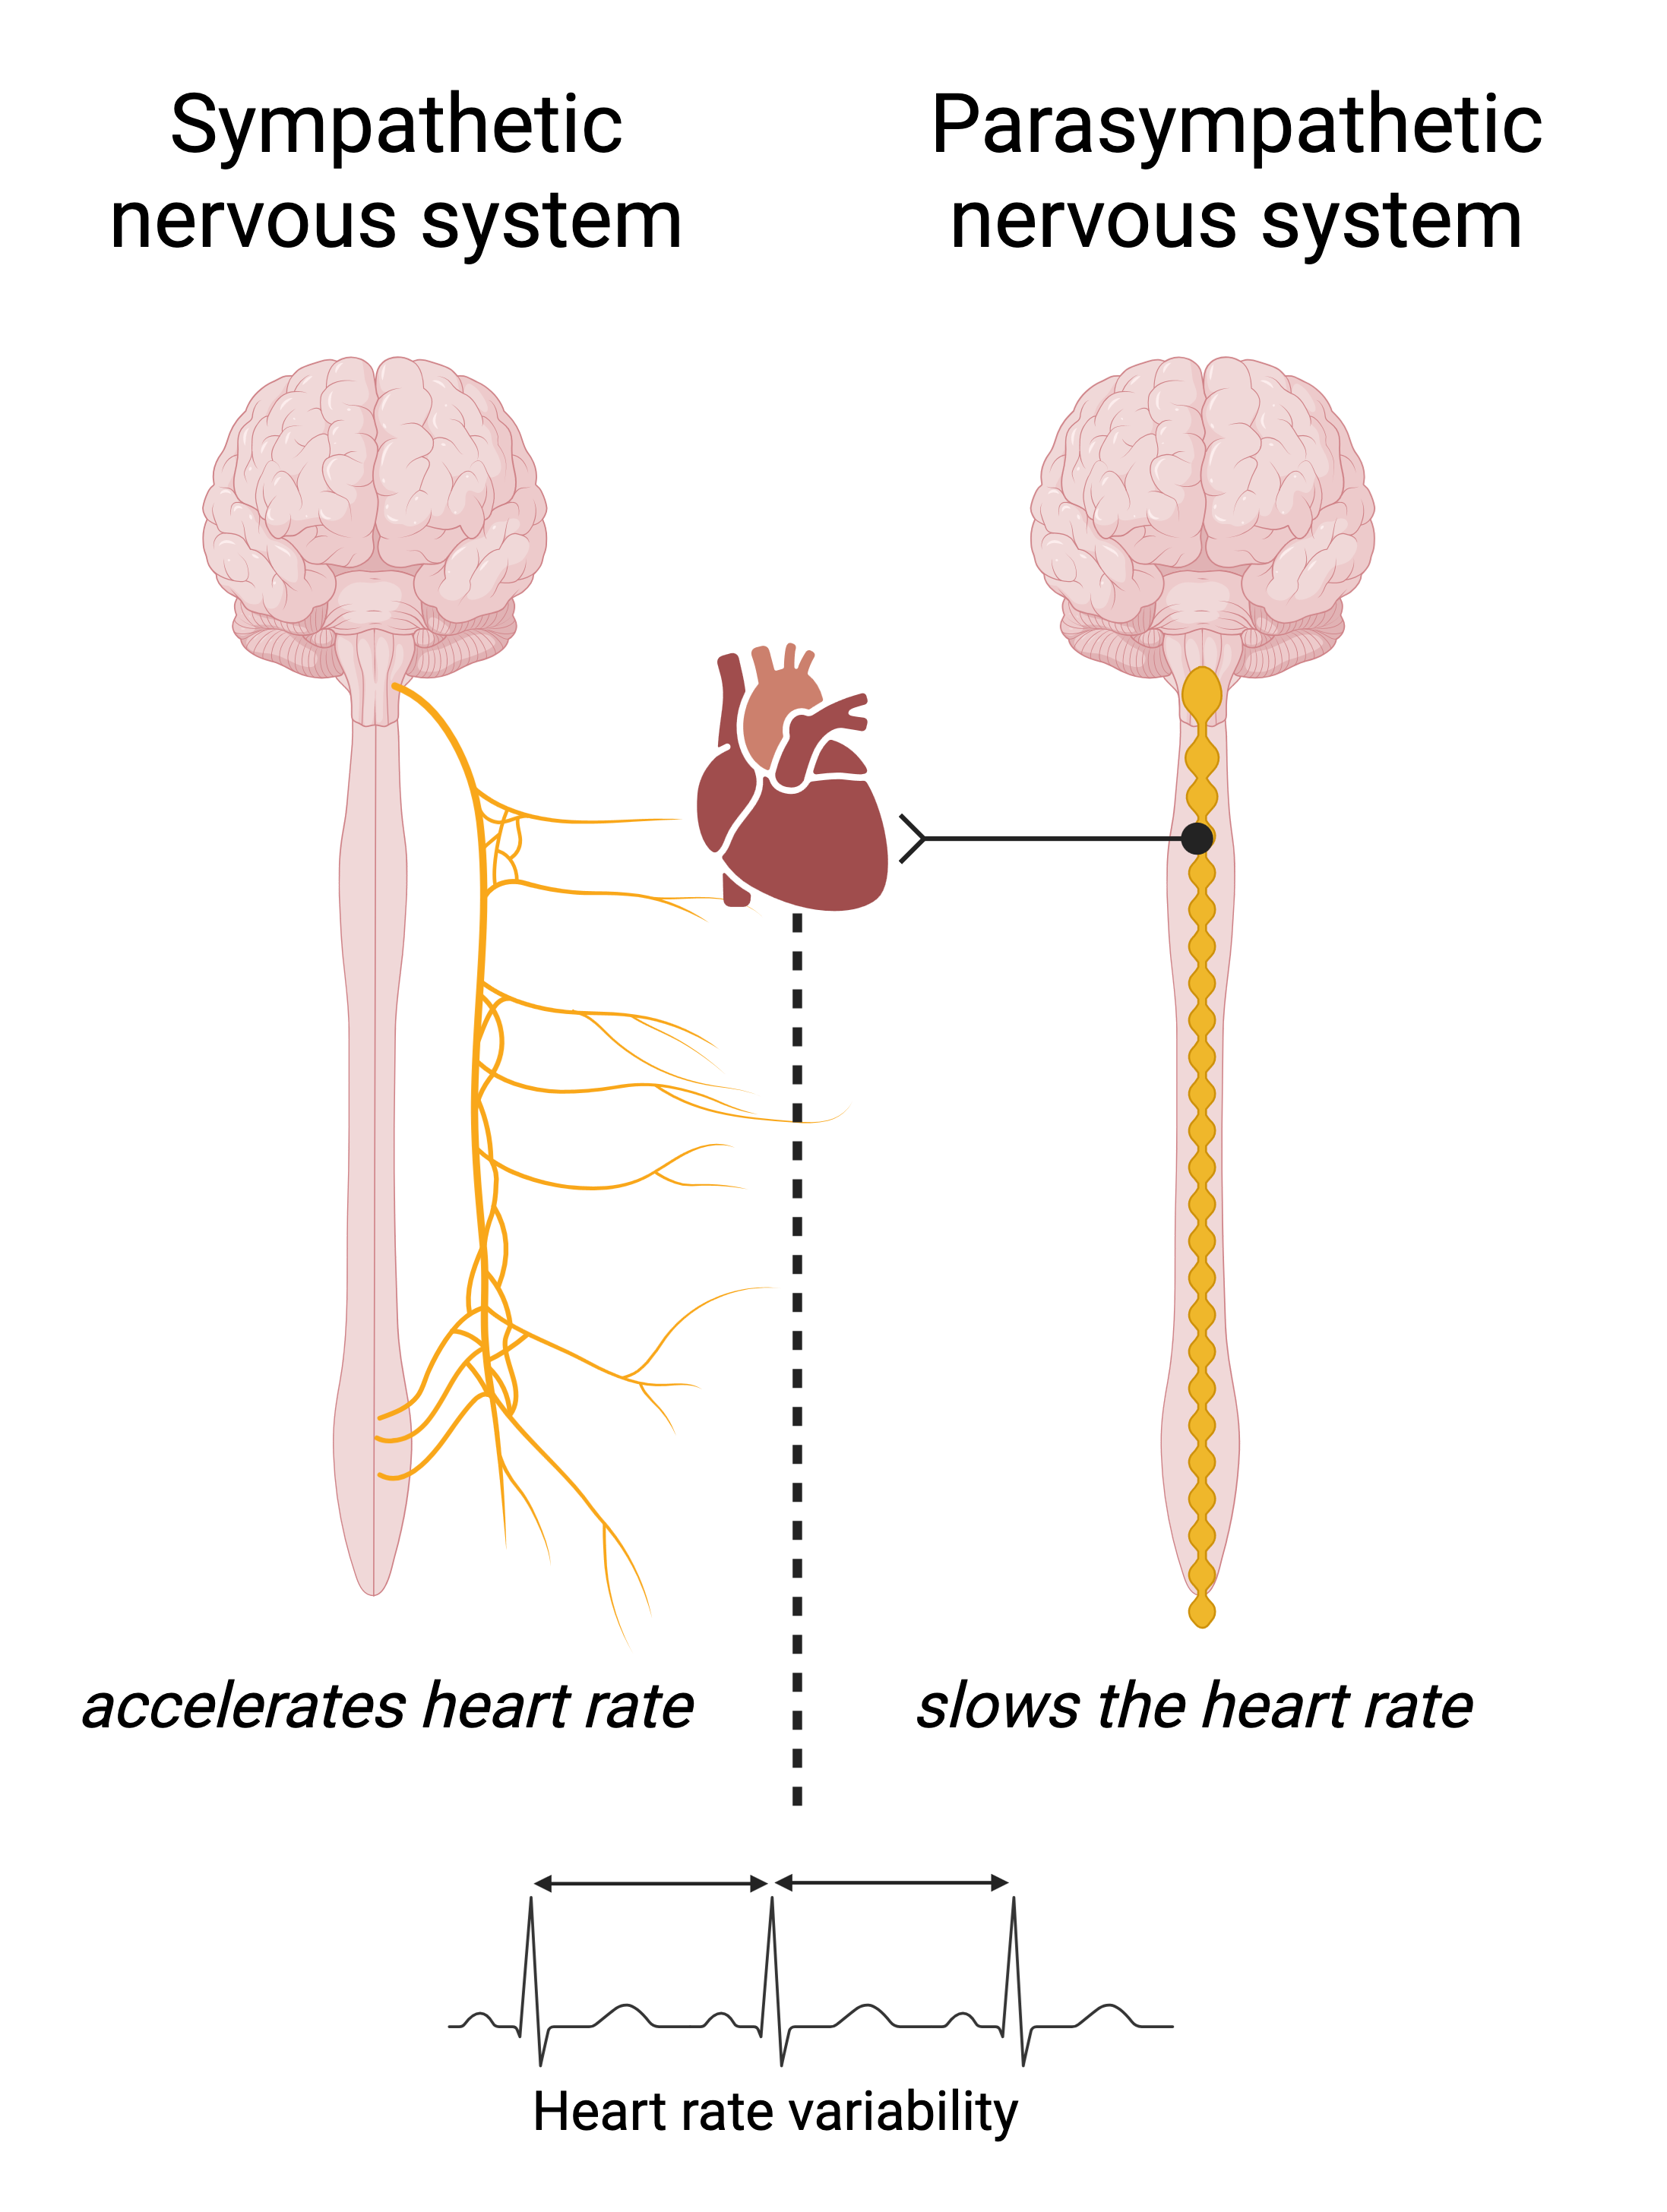
\includegraphics{images/hrv_ans.png} \emph{(Source: Author)}

}

\end{minipage}%

\end{figure}

In youth, the autonomic nervous system is highly adaptive and responsive
to living conditions, maintaining autonomic balance. However, with
aging, there is a gradual decline in parasympathetic function and an
increase in sympathetic activity. Additionally, metabolism-related
conditions such as obesity and diabetes have been shown to further
contribute to cardiovascular autonomic dysfunction (autonomic
dysfunction).\textsuperscript{61} Autonomic dysfunction reflects a
stressed cardiometabolic environment, as both dysfunction in lipid and
glucose metabolism are associated with increased sympathetic
activity.\textsuperscript{61} This dysfunction may result from
cumulative neural damage mediated by mechanisms such as
hyperinsulinemia, insulin resistance, and elevated levels of adipokines.
At the same time, autonomic dysfunction is known to disrupt lipid and
glucose metabolism.\textsuperscript{61} Therefore, the relationship
between autonomic dysfunction and cardiometabolic factors is likely a
vicious cycle.\textsuperscript{62} The consequences can lead to
autonomic dysfunction/neuropathy (CAN), resulting in dysregulation in
heart rate and vascular dynamics. CAN prevalent in 12-73\% in
indiviudals with T2D is liked to CVD diabetic kidney disease, and
all-cause mortality.\textsuperscript{7,63,64} In this dissertation,
`autonomic dysfunction' will be used as the broader term, while `CAN'
will refer specifically to autonomic dysfunction resulting from
neuropathy in diabetes.

Autonomic function can be assessed using heart rate variability (HRV)
indices, which measure the variation in successive normal RR intervals
in milliseconds. HRV provides time- and frequency-domain estimates of
the balance between sympathetic and parasympathetic
activity.\textsuperscript{6} High HRV reflects an autonomic nervous
system with strong adaptability to the body's demands, whereas low
variation indicates poor adaptation to changing conditions. HRV changes
in response to different physiological or environmental conditions
(e.g., sleep, stress, posture, physical activity), and these changes can
be observed in its natural 24-hour (circadian)
pattern.\textsuperscript{13} Most studies have examined autonomic
function using short-term ECG recordings at rest.\textsuperscript{5}
However, extended HRV recordings across the circadian cycle may offer
deeper insights into the influence of lower-frequency variability
sources, such as very-low frequency (0.003--0.04 Hz) and ultra-low
frequency (≤0.003 Hz).\textsuperscript{6} HRV has been applied across
several research domains. For example, in psychology as a marker of
mental stress, in exercise physiology as an indicator of recovery, in
cardiovascular research as a marker of autonomic dysfunction due to
cardiac complications, and in diabetes research as a marker of autonomic
neuropathy.\textsuperscript{7,65--67}T2D alters the expression of
sympathetic bursts, as measured by resting muscle sympathetic nerve
activity (MSNA). MSNA is elevated in individuals with both T2D and
hypertension, compared to those who are normotensive, regardless of
whether they have diabetes or not.\textsuperscript{68} Parasympathetic
activity is also impaired in individuals with high cardiometabolic risk
and T2D, as reflected by reduced baroreflex sensitivity and lower HF and
RMSSD short-term HRV.\textsuperscript{69} Before onset of diabetes and
during progression of diabetes long-term (24-hour) HRV has shown to be
lower compare to those with .\textsuperscript{8,62} Cardiovascular
autonomic reflex tests (CARTs) and orthostatic hypotension are
considered the gold standard for assessing CAN.\textsuperscript{70} The
diagnosis includes assessing pulse rate ratio under test conditions,
such as the deep breathing test, the lying-to-standing test, and the
Valsalva maneuver.\textsuperscript{70} Both HRV and CARTs have shown to
be associated with cardiovascular disease, heart failure, and all-cause
mortality, primarily in populations with T2D or established
cardiovascular disease.\textsuperscript{5,63,71} However, it remains
unclear at which stage in the progression of diabetes risk to
pre-diabetes to diabetes these measures begin to influence the risk of
cardiovascular complications.

\hypertarget{risk-stratification}{%
\section{Risk-stratification}\label{risk-stratification}}

Current cardiopreventive guidelines place strong emphasis on prevention
and treatment of T2D. The 2022 ADA/EASD guidelines for the management of
hyperglycemia in T2D recommend, cardioprotective medication
(glucagon-like peptide-1 receptor agonists {[}GLP-1RA{]} and
Sodium-Glucose Transport Protein 2 inhibitors {[}SGLT2i{]}) as
first-line options for individuals at high cardiovascular
risk.\textsuperscript{72} Due to their benefits in heart failure, SGLT2i
are specifically recommended for patients with documented HFrEF or
HFpEF. High cardiovascular risk is defined as the presence of at least
two risk factors at age \textgreater55 years, such as obesity,
hypertension, smoking, dyslipidemia, or albuminuria.\textsuperscript{72}
However, no additional preclinical markers are recommended to identify
individuals at higher CVD or HF risk or for younger individuals. Despite
their increased risk of cardiovascular complications, individuals at
high risk of developing diabetes remain outside structured treatment
options, even though diabetes risk and cardiometabolic markers can be
successfully modified through lifestyle interventions and medication
such as GLP-1 analogoues.\textsuperscript{73,74} During the progression
and following the onset of T2D, preclinical indicators of CVD risk
become apparent, providing potential opportunities for early risk
stratification. Risk stratification is the process of classifying or
ranking individuals in increasing order of estimated risk, based on risk
scores, biomarker levels, omic data (metabolomic, proteomics, and
genomic) or clinical characteristics.\textsuperscript{75} This approach
aids in identifying patients at highest risk for further prognostic or
diagnostic purposes, identifying subgroups that require further
evaluation, specific treatment, or lifestyle
modifications.\textsuperscript{75}

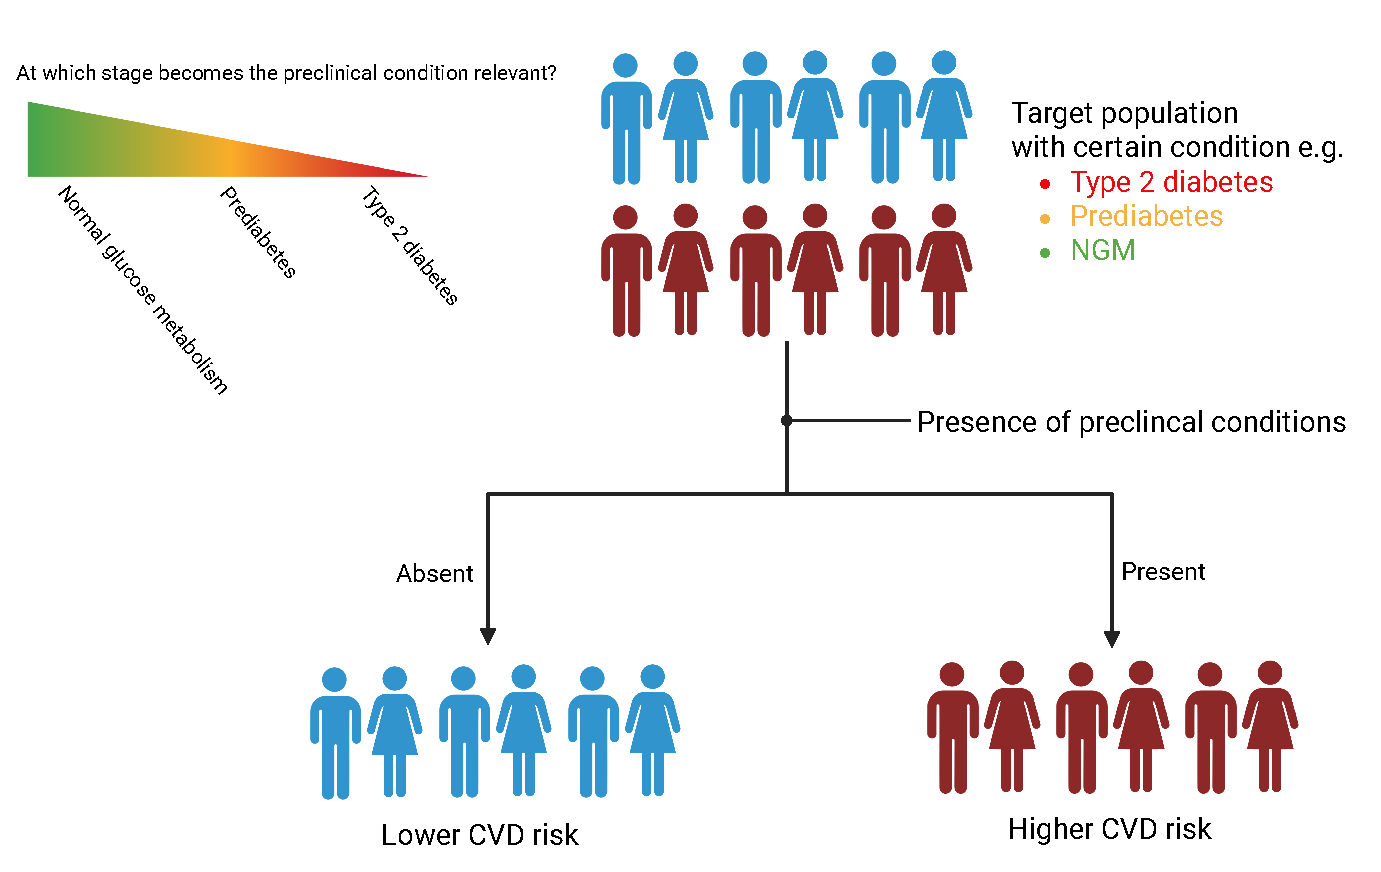
\includegraphics{images/risk_stratification.pdf} \emph{(Source: Author)}

Autonomic dysfunction despite its relationship with cardiovascular
complication has not been used in clinical practice in Denmark. Larger
epidemiological cohort studies encompassing various stages of diabetes
risk, from to prediabetes, onset of T2D, and longer term progression of
T2D, serve as valuable resources for identifying risk-stratification
opportunities. Epidemiological studies provide a broad representation of
the target population, enabling an understanding of the relationship
between autonomic dysfunction and cardiovascular complications across
different levels of care: public health, primary care, and secondary
care. By utilizing observational cohorts, we have the potential to
determine when, along the trajectory of diabetes progression, autonomic
function becomes a meaningful factor for cardiovascular risk
stratification.\textsuperscript{75}

\clearpage
\null
\thispagestyle{empty}
\clearpage

\bookmarksetup{startatroot}

\hypertarget{aim-and-hypothesis}{%
\chapter{Aim and hypothesis}\label{aim-and-hypothesis}}

\clearpage
\null
\thispagestyle{empty}
\clearpage

The overarching hypothesis of this dissertation are that:

• CAN and autonomic dysfunction are associated with CVD and act as an
early risk factor for heart failure and other cardiovascular
complications, including stroke, and myocardial infarction in patients
with prediabetes and/or T2D.

• Autonomic dysfunction is associated with higher levels of sub-clinical
meassures of CVD such as carotid-femoral pulse wave velocity and carotid
artery distensibility.

This dissertation investigates the hypothesis by addressing the
following three aims:

Study I: Quantify the cross-sectional association between 24-hour HRV
and subclinical markers of cardiovascular complications: carotid-femoral
pulse wave velocity and carotid artery distensibility, in participants
with NGM, prediabetes or T2D.

Study II: Quantify the longitudinal association of multiday and hourly
HRV with incidence of ischemic-related CVD, heart failure, and all-cause
mortality in a population with high-risk of diabetes.

Study III: Quantify the cross-sectional association between CAN and
heart failure. Heart failure will be defined by clinical measures
i.e.~N-terminal-pro-BNP (NT-proBNP), WATCH-DM risk, and New York Heart
Association (NYHA) classification scores among individuals with T2D.

\clearpage
\null
\thispagestyle{empty}
\clearpage

\bookmarksetup{startatroot}

\hypertarget{materials-and-methods}{%
\chapter{Materials and methods}\label{materials-and-methods}}

\thispagestyle{empty}
\clearpage

\hypertarget{overview-of-the-studies}{%
\section{Overview of the studies}\label{overview-of-the-studies}}

\begin{longtable}[]{@{}
  >{\raggedright\arraybackslash}p{(\columnwidth - 6\tabcolsep) * \real{0.1900}}
  >{\raggedright\arraybackslash}p{(\columnwidth - 6\tabcolsep) * \real{0.2700}}
  >{\raggedright\arraybackslash}p{(\columnwidth - 6\tabcolsep) * \real{0.2700}}
  >{\raggedright\arraybackslash}p{(\columnwidth - 6\tabcolsep) * \real{0.2700}}@{}}
\caption{Overview of studies}\tabularnewline
\toprule\noalign{}
\begin{minipage}[b]{\linewidth}\raggedright
\end{minipage} & \begin{minipage}[b]{\linewidth}\raggedright
Study I
\end{minipage} & \begin{minipage}[b]{\linewidth}\raggedright
Study II
\end{minipage} & \begin{minipage}[b]{\linewidth}\raggedright
Study III
\end{minipage} \\
\midrule\noalign{}
\endfirsthead
\toprule\noalign{}
\begin{minipage}[b]{\linewidth}\raggedright
\end{minipage} & \begin{minipage}[b]{\linewidth}\raggedright
Study I
\end{minipage} & \begin{minipage}[b]{\linewidth}\raggedright
Study II
\end{minipage} & \begin{minipage}[b]{\linewidth}\raggedright
Study III
\end{minipage} \\
\midrule\noalign{}
\endhead
\bottomrule\noalign{}
\endlastfoot
Title & Cardiovascular autonomic dysfunction is linked with arterial
stiffness across glucose metabolism: The Maastricht Study &
Cardiovascular autonomic dysfunction precedes cardiovascular disease and
all-cause mortality: 11-year follow-up in the ADDITION-PRO study &
Cardiovascular autonomic neuropathy and subclinical heart failure in
T2D: The CANCAN study \\
Design & Aetiological cross-sectional study & Aetiological prospective
cohort study & Descriptive cross-sectional study \\
Cohort & Maastricht study & ADDITION-PRO study & CANCAN study \\
Study population & 3673 individuals with NGM, prediabetes, or T2D & 2082
individuals with high risk of diabetes & 176 patients with T2D visiting
outpatients clinics \\
Data sources & Observational phenotyping cohort from The Maastricht
Study in the Netherlands & Cohort study of selected individuals based on
having high risk of diabetes & Clinical cohort study \\
Determinant & 24-hour HRV & Multiday and hourly HRV & Cardiovascular
autonomic reflex test \\
Primary outcome & Arterial stiffness & Major adverse cardiovascular
events, heart failure, and all-cause mortality & NT-proBNP, NYHA
classification, and WATCH-DM risk score \\
Statistical analysis & Linear regression & Poisson regression & Logistic
regression \\
Missing data & Complete case analysis & Multiple imputation of chained
equations for confounders & Complete case analysis and multiple
imputation of chained equations for CART and confounders \\
\end{longtable}

\hypertarget{study-population}{%
\subsection{Study population}\label{study-population}}

\begin{figure}

{\centering 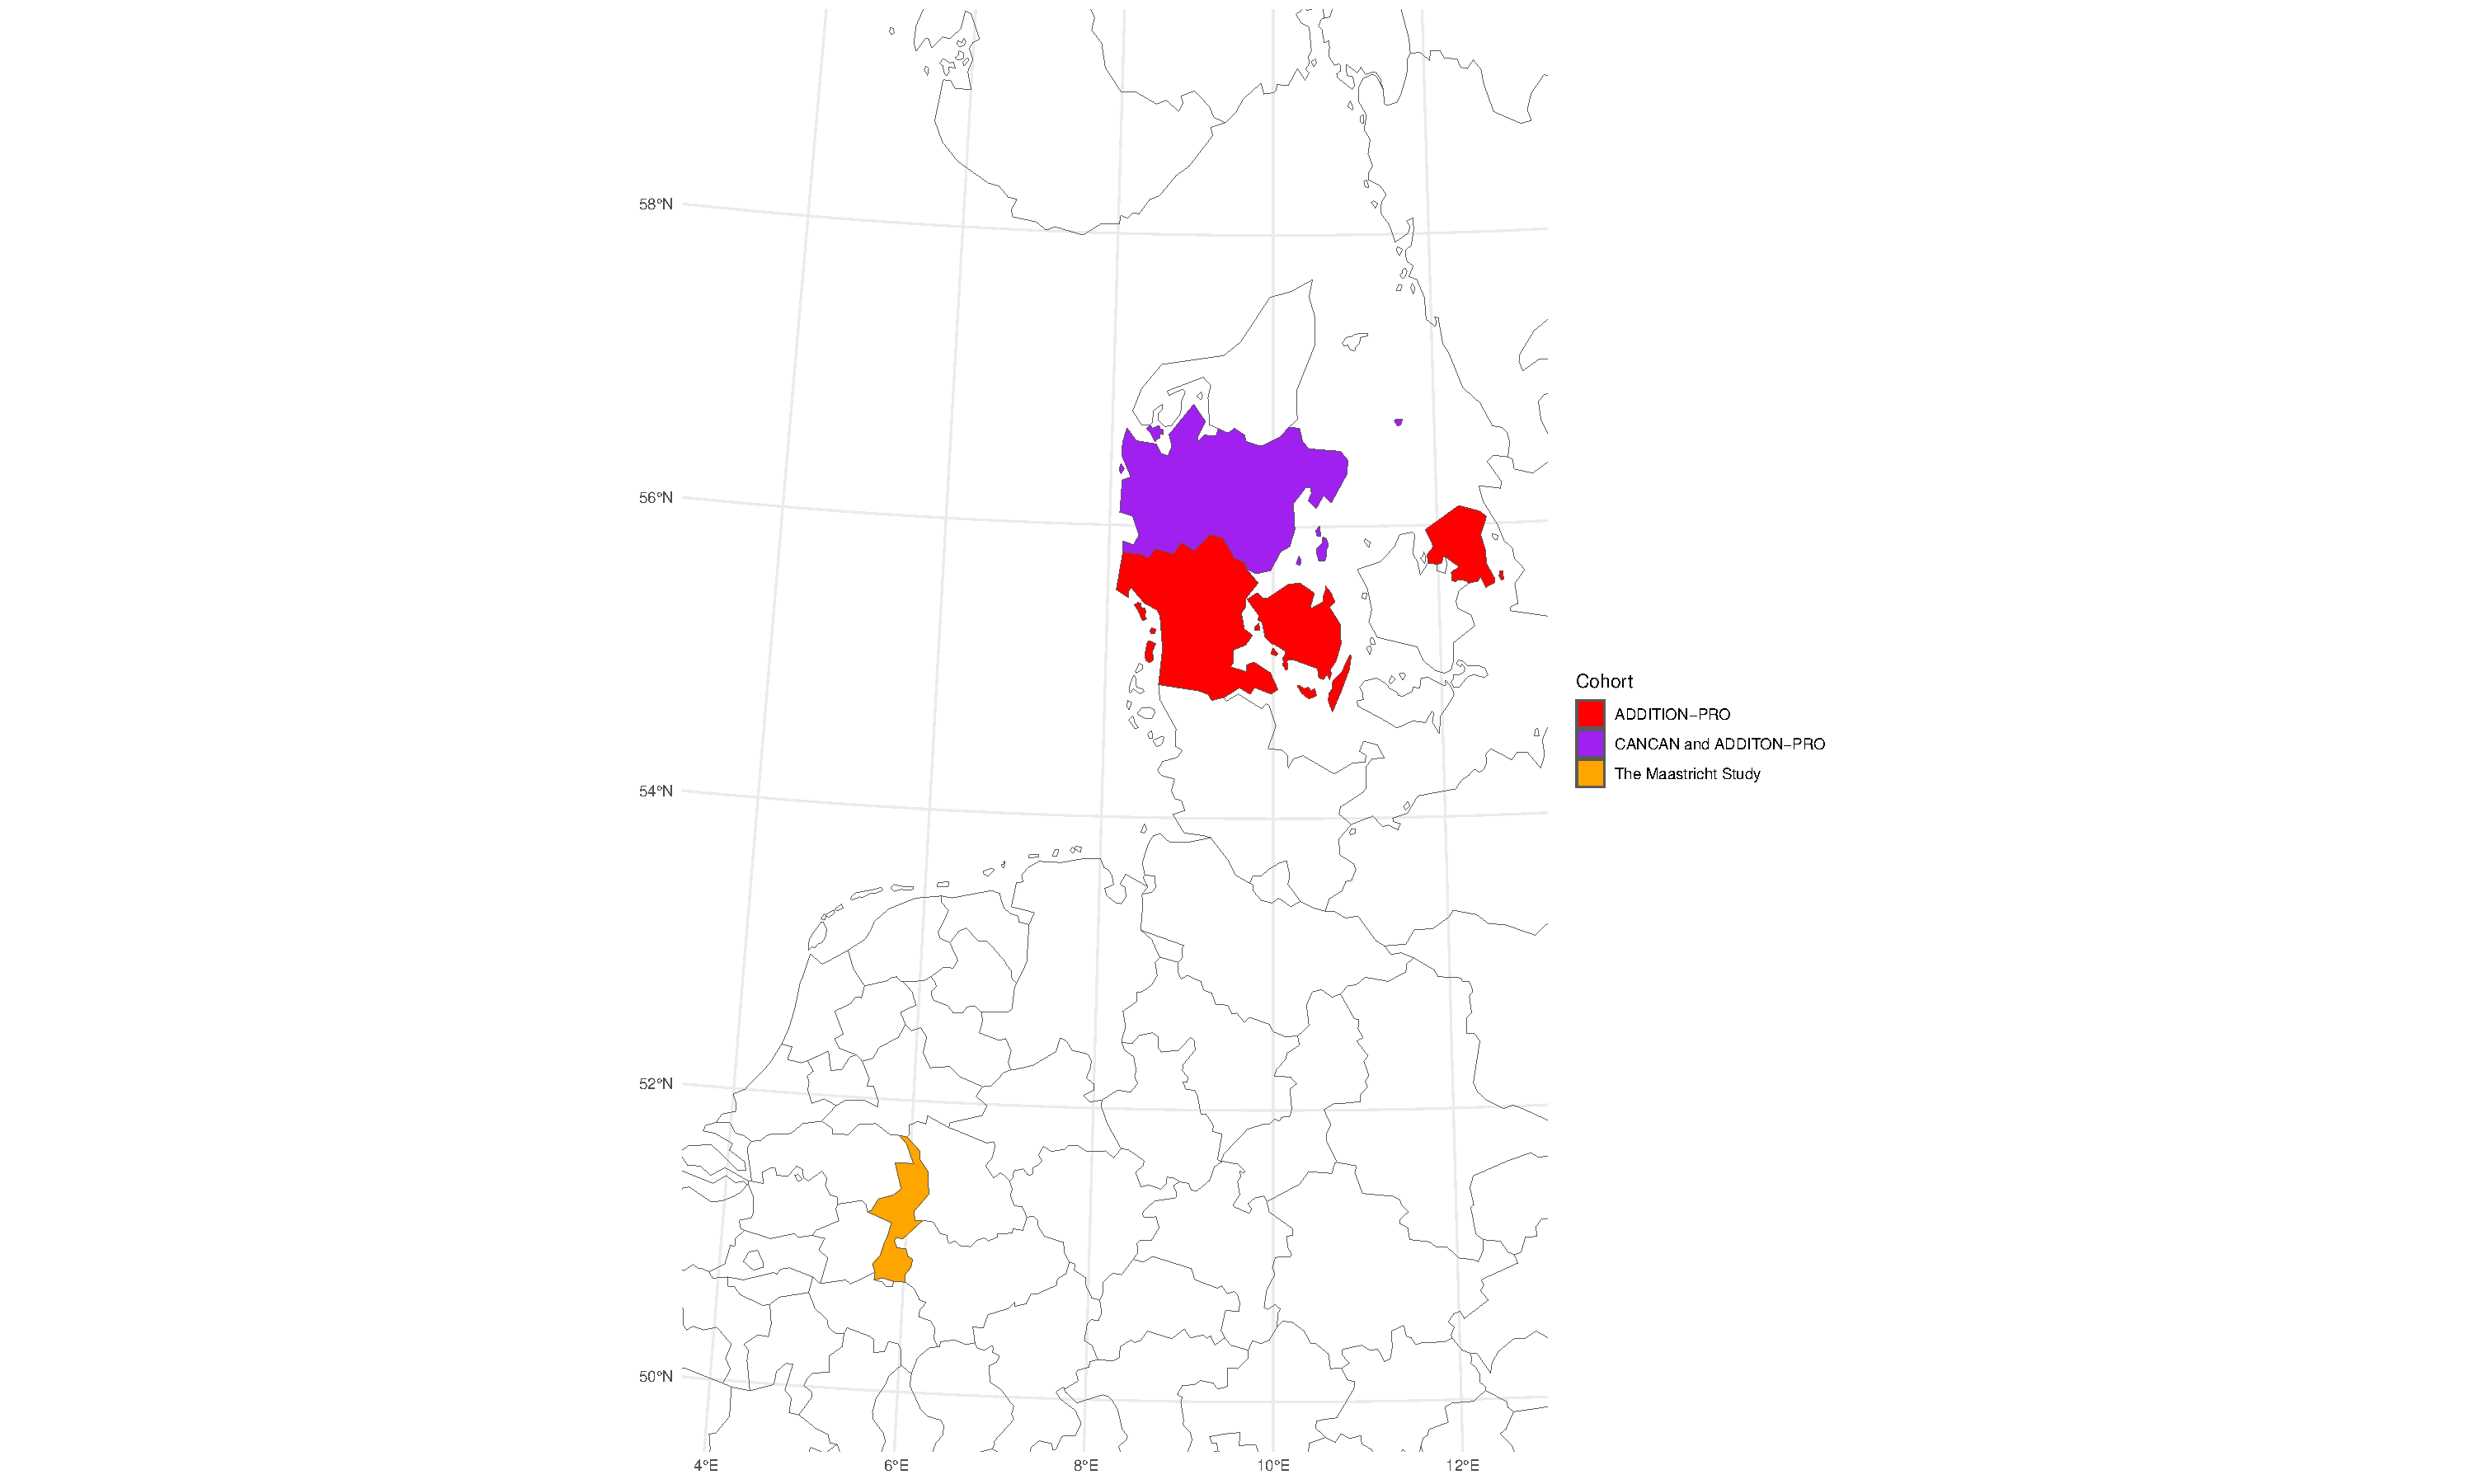
\includegraphics[width=8in,height=\textheight]{images/cohort_map.pdf}

}

\caption{\textbf{Map of Study populations}}

\end{figure}

\hypertarget{study-i---the-maastricht-study}{%
\subsubsection{Study I - The Maastricht
Study}\label{study-i---the-maastricht-study}}

The Maastricht Study is a prospective, observational phenotyping study
of the general population in the province of Limburg, located in the
southern part of the Netherlands. The recruitment of individuals with
T2D was emphasized through the regional Diabetes Patient Registry, with
the aim of extensively phenotyping individuals with T2D and those in
intermediate stages of the disease. Eligibility criteria included an age
range of 40--70 years. Participants were recruited through mass media
campaigns and mailings from municipal registries (Gemeentelijke Basis
Administratie; GBA).\textsuperscript{76} In the analysis of Study I, the
study among 7449 individuals included participants with measurements of
24-hour HRV and at least one measure of arterial stiffness
(carotid-femoral pulse wave velocity or carotid artery distensibility),
both of which were completed within a three-month period between
November 2010 and December 2020. Among those participants with prior CVD
were excluded\textsuperscript{77}. Approval was granted by the
institutional medical ethics committee (NL31329.068.10) and the Minister
of Health, Welfare and Sports of the Netherlands (Permit
131088-105234-PG). Written informed consent was given by all
participants.\textsuperscript{77}

\hypertarget{study-ii---addition-pro}{%
\subsubsection{Study II - ADDITION-PRO}\label{study-ii---addition-pro}}

The ADDITION-PRO study is a prospective, population-based cohort nested
within the Danish arm of the ADDITION-Europe study. ADDITION was
originally designed as a stepwise screening program for T2D in general
practice, with the aim of identifying individuals with screen-detected
T2D for recruitment into the ADDITION trial. The objective of
ADDITION-PRO is to investigate early markers of CVD and metabolic
dysfunction in individuals in different tiers of diabetes risk.

The ADDITION-Europe screening program identified a large number of
individuals with impaired fasting glucose (IFG), impaired glucose
tolerance (IGT), and normoglycemia despite having risk factors for
diabetes and CVD. Participants for ADDITION-PRO were recruited from the
original ADDITION-DK screening cohort, which included individuals from
190 general practices across Denmark. The recruitment strategy focused
on individuals at high risk of diabetes without T2D, identified through
a stepwise screening program that incorporated the Danish diabetes risk
score from the Inter99 study\textsuperscript{78}. This assessment,
conducted between 2001 and 2006, considered factors such as age, sex,
history of gestational diabetes, family history of diabetes, known
hypertension, BMI, and physical activity. High-risk individuals were
further screened for T2D using blood measurements, including HbA1c,
random blood glucose, FPG, and OGTT. Those with screen-detected
diabetes, confirmed by a second OGTT, were invited to participate in the
ADDITION trial. High risk individuals without T2D were further
considered in as the sampling frame for ADDITION-PRO.

Between 2009 and 2011, a follow-up health examination was conducted at
four ADDITION-DK study centers to establish a cohort baseline. Eligible
participants were those still alive, residing near the research centers
(Steno Diabetes Center Copenhagen, Aarhus University Hospital, Holstebro
Hospital, and the Hospital of South West Jutland, Esbjerg), and who had
not withdrawn consent. Eligibility criteria included individuals aged
40--70 years who had previously undergone diabetes screening in
ADDITION-DK. Exclusion criteria included pregnancy, psychological or
psychiatric disorders preventing informed consent, and life-limiting
conditions. One key feature of the data collection was the precise
measurement of physical activity and energy expenditure using a combined
chest-worn accelerometer/heart rate monitor (ActiHeart), which recorded
acceleration and heart rate over a week. In Study II, participants with
at least a 48-hour recording were included for the primary analysis, and
then participants with hourly measures of physical acceleration during
the hourly HRV recording were included in the second analysis.
Participants with prior CVD ten years before inclusion were also
excluded.

Disease history and follow-up data for the population were obtained from
Denmark's national registry system, which allows linkage of health
records using the personal Civil Registration Number assigned to all
citizens. The following national registries were accessed to collect
information on incident CVD and mortality, medication use, and
healthcare utilization: the National Patient Registry (hospital
admissions and outpatient contacts), the National Health Service
Registry (general practice visits), the Medical Prescription Registry,
the Diabetes Registry, and the Cause of Death Registry.

\hypertarget{study-iii---cancan}{%
\subsubsection{Study III - CANCAN}\label{study-iii---cancan}}

The CANCAN Study is an observational study conducted at two hospital
outpatient clinics: Viborg Regional Hospital and Regional Hospital
Gødstrup. The aim is to implement a screening protocol for identifying
high-risk individuals using CAN assessments, continuous glucose
monitoring, and heart failure indicators. All measures were part of
routine clinical care for T2D in Central Denmark. A total of 200 adults
(\textgreater18 years) with T2D and a disease duration of over one year
were included. Exclusion criteria were recent laser-treated eye disease
(≤3 months), pregnancy, lactation, life-threatening illness, or
cognitive impairment preventing consent. Participants were identified
via electronic records and were informed about the study by their doctor
during a telephone call. Those interested were invited to attend a
dedicated meeting before their annual diabetes exam, during which study
details were discussed. Recruitment was conducted from 2021 to 2024. In
Study III, participants without a valid NT-proBNP measurement were
excluded.

\hypertarget{study-variables}{%
\section{Study variables}\label{study-variables}}

\hypertarget{measures-for-autonomic-dysfunction-neuropathy}{%
\subsection{Measures for autonomic dysfunction/
neuropathy}\label{measures-for-autonomic-dysfunction-neuropathy}}

\begin{figure}

{\centering 

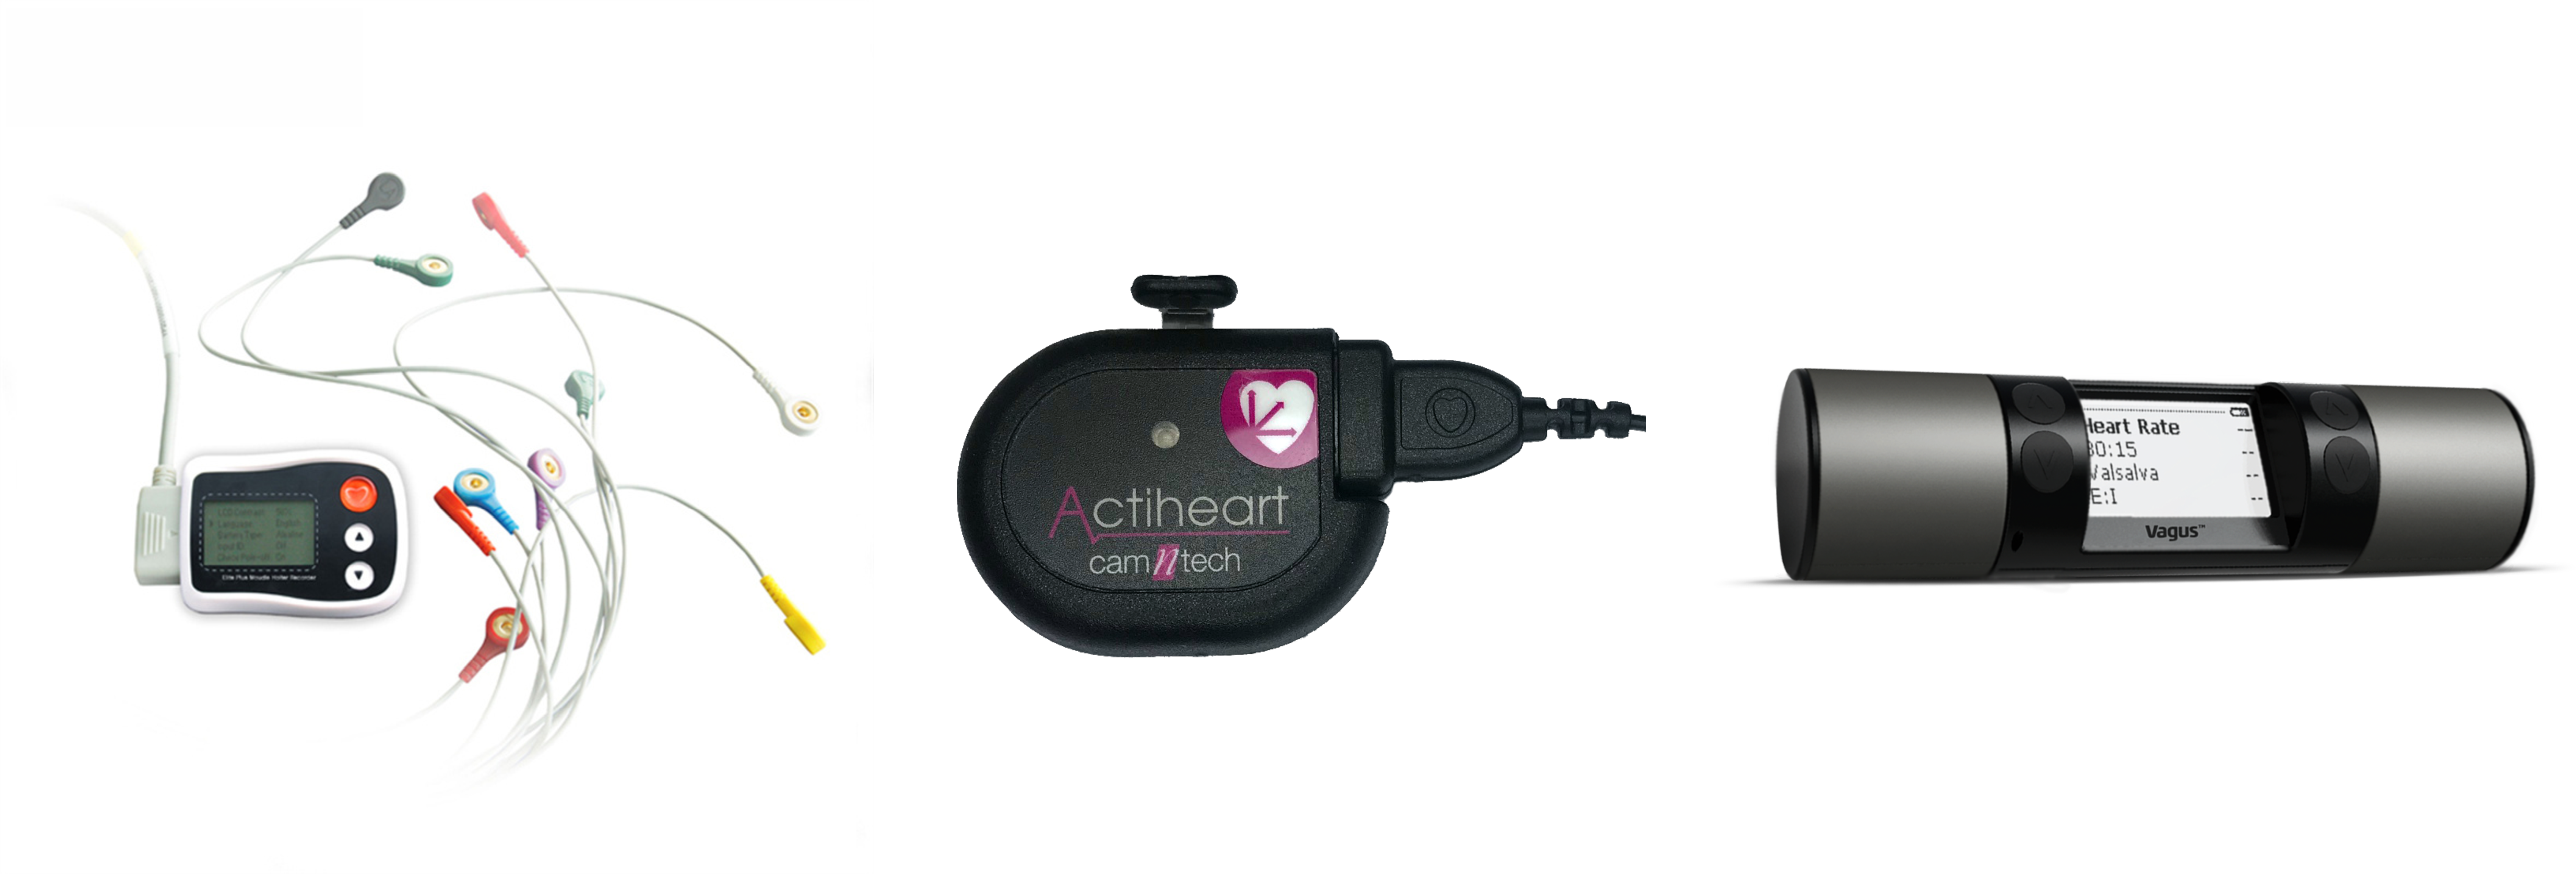
\includegraphics{images/can_tools.pdf} \emph{Left: Holter monitor;
Middle: Actiheart; Right: Vagus™ device}

}

\caption{\label{fig-monitor}\textbf{Heart rate monitors}}

\end{figure}

\textbf{Heart rate variability}

In Studies I--III, different devices were used to capture the distance
between each heartbeat, defined as RR intervals, from electrocardiogram
traces---either directly from heartbeat traces or indirectly from pulse
traces. From these, a sequence of successive heartbeat intervals was
extracted to calculate time- and frequency-domain HRV.

\begin{figure}

{\centering 

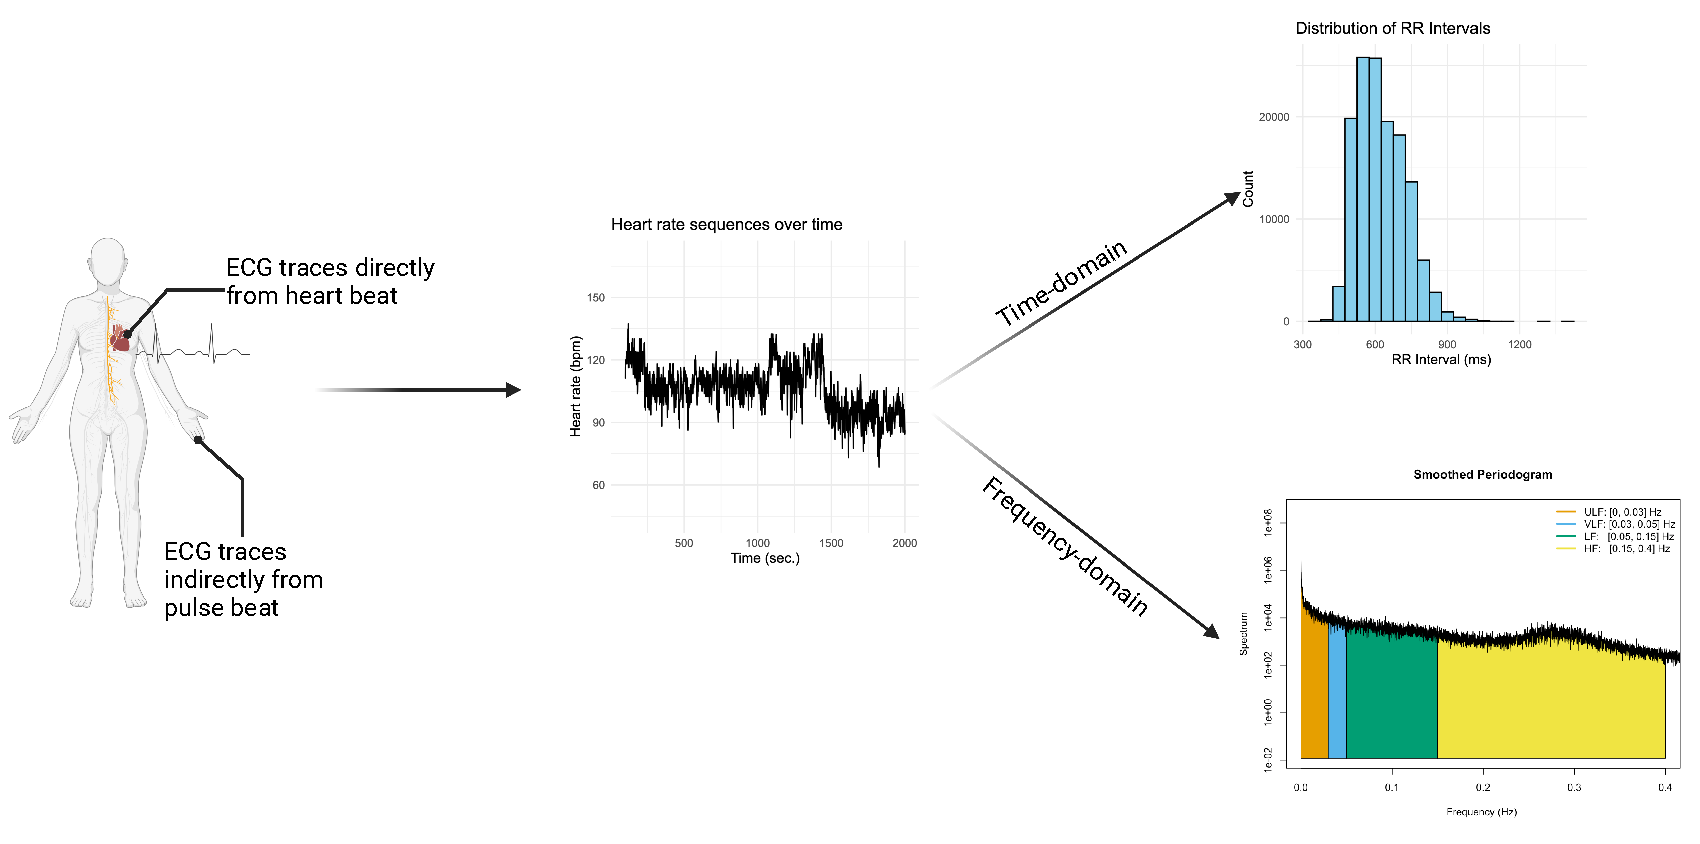
\includegraphics{images/measurements_hrv.pdf} \emph{Time- and Frequency
domain HRV indices (Source: Author)}

}

\caption{\label{fig-hrv}\textbf{Heart rate variability calculations}}

\end{figure}

\emph{Time-domain indices}

Time-domain measures of HRV are based on the statistical distribution of
normal-to-normal (NN) heartbeat intervals. Descriptions of time-domain
indices are summarized in Table~\ref{tbl-td}.

\hypertarget{tbl-td}{}
\begin{longtable}[]{@{}
  >{\raggedright\arraybackslash}p{(\columnwidth - 2\tabcolsep) * \real{0.4000}}
  >{\raggedright\arraybackslash}p{(\columnwidth - 2\tabcolsep) * \real{0.6000}}@{}}
\caption{\label{tbl-td}\textbf{Box 1} Time-domain indices reflections of
autonomic function}\tabularnewline
\toprule\noalign{}
\begin{minipage}[b]{\linewidth}\raggedright
Time-domain HRV
\end{minipage} & \begin{minipage}[b]{\linewidth}\raggedright
Description
\end{minipage} \\
\midrule\noalign{}
\endfirsthead
\toprule\noalign{}
\begin{minipage}[b]{\linewidth}\raggedright
Time-domain HRV
\end{minipage} & \begin{minipage}[b]{\linewidth}\raggedright
Description
\end{minipage} \\
\midrule\noalign{}
\endhead
\bottomrule\noalign{}
\endlastfoot
\textbf{Standard deviation of NN heart beat intervals (SDNN, in ms)} &
Measures the total variation in interbeat intervals and reflects both
sympathetic and parasympathetic activity\textsuperscript{6}. \\
\textbf{SD of the averages of NN intervals in 5-minute segments
throughout the recording (SDANN, in ms)} & Measures variations in
5-minute mean interbeat intervals, primarily reflecting autonomic
fluctuations associated with the circadian rhythm\textsuperscript{6} \\
\textbf{Mean of the SDs of all NN intervals for all 5-minute segments
(SDNN index, in ms)} & Measures the average short-term variability in
interbeat intervals across successive 5-minute periods, reflecting both
sympathetic and parasympathetic modulation of heart
rate\textsuperscript{6} \\
\textbf{NN50 count divided by the total number of all NN intervals
(pNN50, percentage)} & Measures the proportion of successive interbeat
intervals differing by more than 50 ms, primarily reflecting
parasympathetic (vagal) activity\textsuperscript{79}. \\
\textbf{Square root of the mean of the sum of squares of differences
between adjacent NN intervals (RMSSD, in ms)} & Measures variation in
successive interbeat intervals during inhalation and exhalation,
primarily reflecting parasympathetic (vagal)
activity\textsuperscript{79} \\
\end{longtable}

\emph{Frequency-domain indices}

Frequency-domain HRV indices are derived from sequences of NN intervals
that have been transformed into the spectral domain using Fourier
transformation. These indices quantify heart rate oscillations over
different timescales. Short-term variations, such as respiratory sinus
arrhythmia, are reflective of rapid autonomic changes, while longer
oscillations are indicative of autonomic responses to posture changes,
circadian rhythms, or other physiological processes. Descriptions of
frequency-domain indices are summarized in Table~\ref{tbl-fq}. .

\hypertarget{tbl-fq}{}
\begin{longtable}[]{@{}
  >{\raggedright\arraybackslash}p{(\columnwidth - 2\tabcolsep) * \real{0.4000}}
  >{\raggedright\arraybackslash}p{(\columnwidth - 2\tabcolsep) * \real{0.6000}}@{}}
\caption{\label{tbl-fq}\textbf{Box 2} Frequency-domain indices
reflections of autonomic function}\tabularnewline
\toprule\noalign{}
\begin{minipage}[b]{\linewidth}\raggedright
Frequency domain HRV
\end{minipage} & \begin{minipage}[b]{\linewidth}\raggedright
Description
\end{minipage} \\
\midrule\noalign{}
\endfirsthead
\toprule\noalign{}
\begin{minipage}[b]{\linewidth}\raggedright
Frequency domain HRV
\end{minipage} & \begin{minipage}[b]{\linewidth}\raggedright
Description
\end{minipage} \\
\midrule\noalign{}
\endhead
\bottomrule\noalign{}
\endlastfoot
\textbf{Variance of all NN intervals ≤ 0.4 Hz, total power (TP, in ms²)}
& Measures the total variation in interbeat intervals, reflecting both
short- and long-term autonomic regulation by the sympathetic and
parasympathetic nervous system.\textsuperscript{6} \\
\textbf{Ultra low-frequency range (ULF, in ms² ≤ 0.003 Hz)} & Measures
very long-term oscillations in interbeat intervals, influenced by
autonomic responses to circadian rhythms, physical activity, metabolic
processes, and thermoregulation.\textsuperscript{80,81} \\
\textbf{Very-low-frequency range (VLF, in ms²; 0.003--0.04 Hz)} &
Measures oscillations in interbeat intervals over 5-minute periods,
reflecting the activity of the renin--angiotensin system and peaks in
sympathetic nervous system activity, while also depending on
parasympathetic modulation.\textsuperscript{82,83} \\
\textbf{Low-frequency range (LF, in ms²; 0.04--0.15 Hz)} & Measures
intermediate oscillations in interbeat intervals, reflecting a
combination of sympathetic and parasympathetic nervous system activity,
particularly associated with baroreflex function and blood pressure
regulation.\textsuperscript{84} \\
\textbf{High-frequency range (HF, in ms²; 0.15--0.4 Hz)} & Measures
short-term oscillations during inspiration and expiration, reflecting
parasympathetic modulation of heart rate via the vagus nerve, and
closely associated with respiratory sinus
arrhythmia.\textsuperscript{85} \\
\end{longtable}

\textbf{Holter recordings in study I}

All ECG recordings were obtained using a 12-lead Holter system
(Fysiologic ECG Services, Amsterdam, the Netherlands) over 24 hours, as
previously described.\textsuperscript{76} Participants were instructed
to follow their regular daily activities but avoid showering during the
recording. The ECG data were processed using proprietary Holter Analysis
Software (Fysiologic ECG Services), where artefacts and ectopic beats
were excluded through automated processing and manual validation. A
minimum recording duration of 18 hours was required for further
analysis.\textsuperscript{8,77} Inter-beat intervals between consecutive
sinus beats were provided in milliseconds (ms). Time-domain HRV indices
were calculated, including SDNN, SDANN, RMSSD, SDNN index, and pNN50.
Frequency-domain measures were derived using Fast Fourier Transform,
including TP, ULF, VLF, LF, and HF.\textsuperscript{77}Outliers were
removed. HRV indices were standardised by their mean and SD, and
composite Z-scores were computed for time and frequency-domain measures,
respectively. This selection of indices covers the main sources of HRV
variance.\textsuperscript{77}

\textbf{ActiHeart heart rate and physical activity in study II}

Heart rate was measured using a combined accelerometer and heart rate
monitor (ActiHeart, CamNTech, Cambridge, UK), which recorded uniaxial
acceleration and heart rate. The data collection and processing methods
have been described previously. Mean heart rates were recorded in
30-second epochs. Based on an algorithm, distributions of inter-beat
intervals were calculated in each 30-second epoch.\textsuperscript{86}
HRV calculations were performed using the RHRV package (version 4.2.7)
in R.\textsuperscript{86,87} The algorithm was tested on a dataset with
full access to all inter-beat intervals.\textsuperscript{86} HRV indices
based on global distribution in 24-hour recordings showed high
validity.\textsuperscript{87} HRV indices including SDNN, SDANN, SDNN
index, TINN, and mean heart rate (HR) were calculated by week, 24-hour
cycle, and hour of the day, with hourly values averaged across recording
days.\textsuperscript{87}

\textbf{Vagus device for cardiovascular autonomic reflex test in study
III}

CAN was diagnosed using cardiovascular autonomic reflex tests (CARTs),
the gold standard for CAN assessment. R-R intervals were derived from an
ECG signal using the Vagus™ device (Medicus Engineering, Aarhus,
Denmark).\textsuperscript{70,88} Pulse rate ratios were measured under
different conditions.\textsuperscript{88} Three standardized
cardiovascular autonomic reflex tests (CARTs) were performed: (1)
lying-to-standing, (2) deep breathing, and (3) the Valsalva manoeuvre,
following a standardized protocol conducted between 8:00 a.m. and 2:00
p.m., after 10 minutes of supine rest.\textsuperscript{88} Smoking and
caffeine intake were prohibited two hours before testing. Each test was
conducted once by trained examiners.\textsuperscript{88}

Manifest CAN was defined as two or more abnormal CARTs using
age-specific formula.\textsuperscript{70} The Vagus™ device's accuracy
has been validated against FDA standards and stationary devices, showing
moderate to high reproducibility.\textsuperscript{89} Orthostatic
hypotension was defined as a sustained drop in systolic blood pressure
of ≥20 mmHg or diastolic blood pressure of ≥10 mmHg within three minutes
of standing.\textsuperscript{88}

\begin{figure}

{\centering 

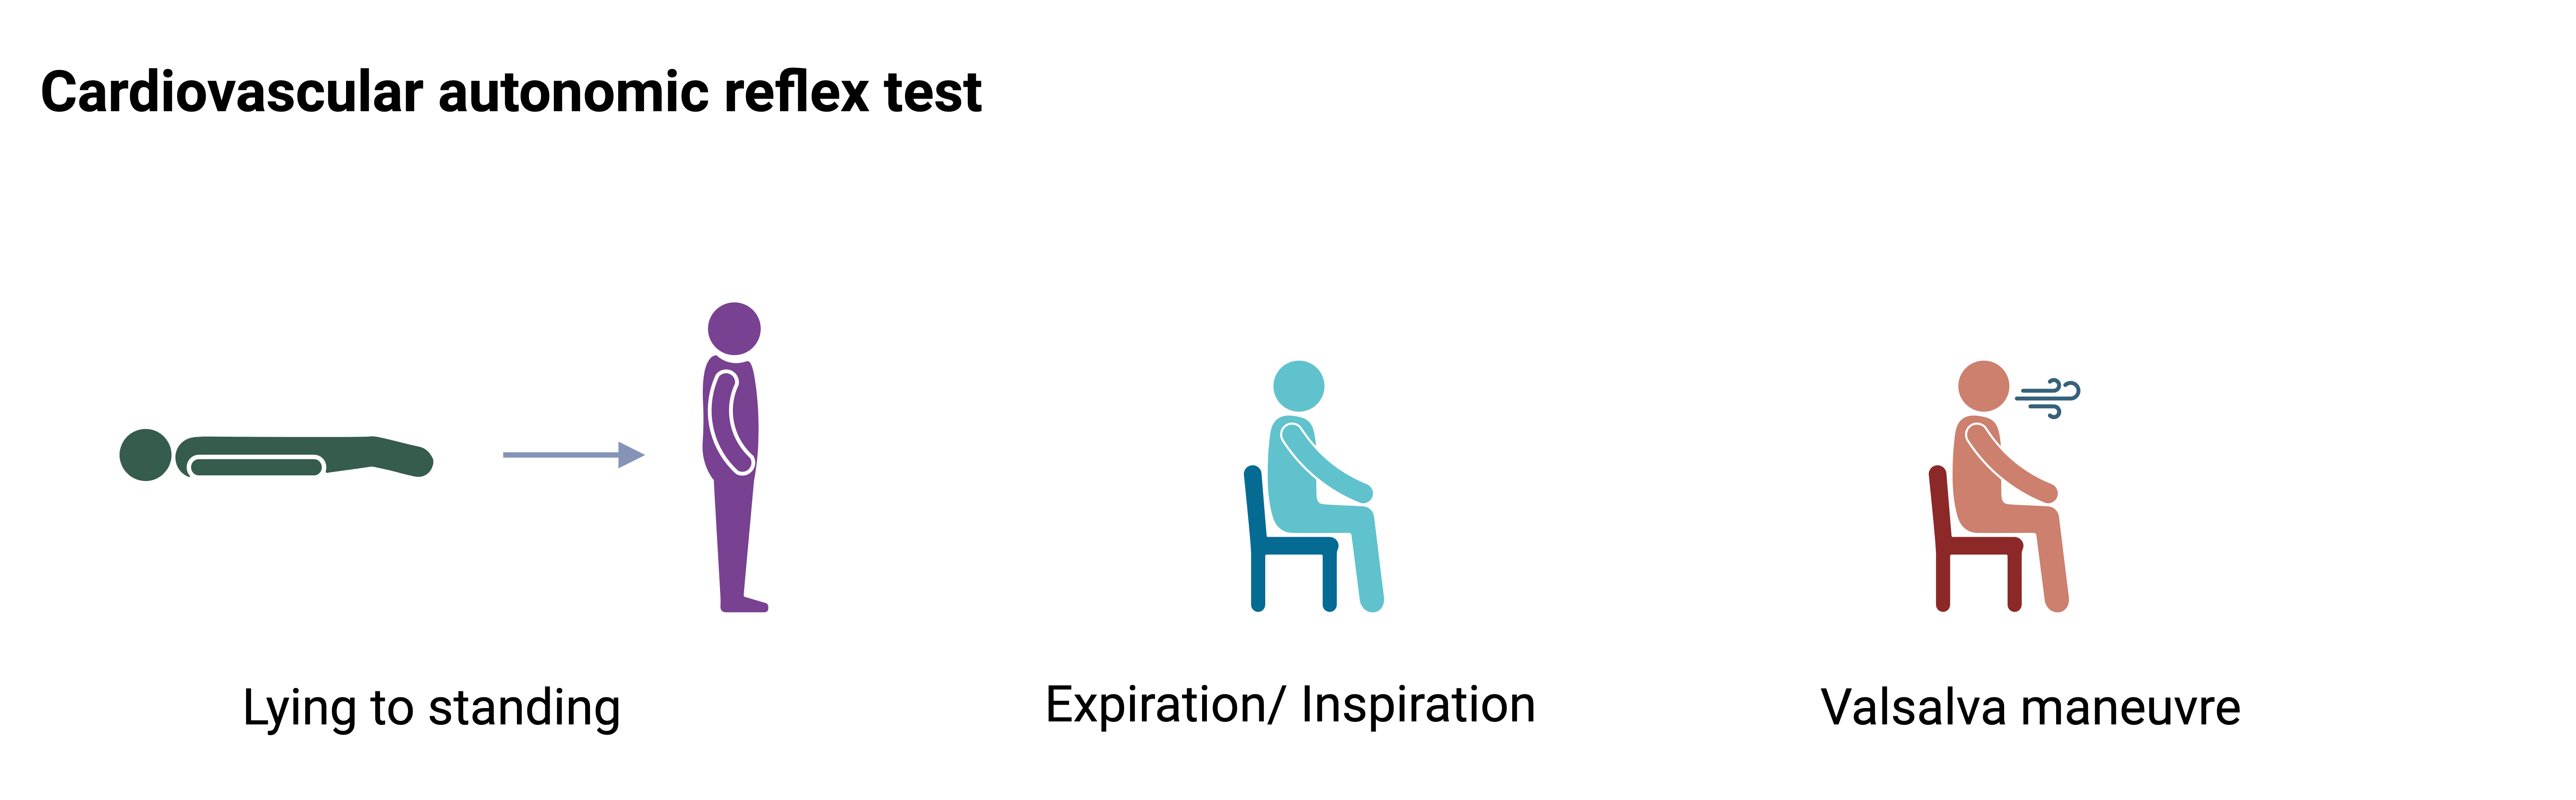
\includegraphics{images/cart.png} \emph{(source: Author)}

}

\caption{\label{fig-cart}\textbf{Cardiovascular autonomic reflex test}}

\end{figure}

\hypertarget{confounders-and-variables-for-instrumental-bias}{%
\subsection{Confounders and variables for instrumental
bias}\label{confounders-and-variables-for-instrumental-bias}}

Across Studies I, II, and III, a comprehensive set of covariates and
potential confounders was assessed, including lifestyle factors,
clinical measurements, biochemical markers, and socioeconomic
indicators.\textsuperscript{77,87,88}

Smoking status was self-reported in all studies and categorized as
never, former, or current (Study I); current/ex/never (Study II); and
smoker/non-smoker (Study III). Alcohol consumption was recorded as
average weekly units in all three studies.\textsuperscript{77,87,88}
Physical activity was assessed via self-report in Studies I, II, and
III. In Study I, total and moderate-to-vigorous activity (hours/week)
was recorded. Study II used the Recent Physical Activity Questionnaire
(RPAQ) to calculate physical activity energy expenditure (PAEE), while
Study III classified activity as sedentary or
non-sedentary.\textsuperscript{77,87,88} In addition, Study II used
combined accelerometry and heart rate monitoring (ActiHeart) to estimate
PAEE.\textsuperscript{87} Register-based data on socioeconomic status at
baseline, including education length, income, and employment status,
were included in Study II.\textsuperscript{87} All studies included
measurements of body mass index (BMI), waist circumference, and systolic
and diastolic blood pressure, obtained during clinical
examinations.\textsuperscript{77,87,88}

Blood samples were analyzed in all studies for HbA1c, fasting plasma
glucose (FPG), triglycerides, total cholesterol, high-density
lipoprotein (HDL), and low-density lipoprotein (LDL)
cholesterol.\textsuperscript{77,87,88} Study I also included a 2-hour
oral glucose tolerance test (OGTT) to classify glucose metabolism status
based on FPG and OGTT (normal, prediabetes, T2D) using WHO 2006
criteria, excluding HbA1c as a diagnostic criterion.\textsuperscript{77}
Study III additionally measured creatinine, estimated glomerular
filtration rate (eGFR), and urine albumin-to-creatinine
ratio.\textsuperscript{88}

Self-reported history of CVD and use of anti-hypertensive,
glucose-lowering, and lipid-lowering medications were collected in all
studies.\textsuperscript{77,87,88} In Study II, history of CVD events in
the 10 years prior to baseline was retrieved from national
registers.\textsuperscript{87} In Study III, history of CVD was
collected from electronic patient records.\textsuperscript{88}

\hypertarget{outcomes}{%
\section{Outcomes}\label{outcomes}}

\hypertarget{arterial-stiffness}{%
\subsection{Arterial stiffness}\label{arterial-stiffness}}

Arterial stiffness is characterized by arteriosclerosis and
atherosclerosis properties of the arteries. The stiffness of different
segments of the vascular musculature can be assessed both locally and
dynamically. Aortic and carotid stiffness were assessed as markers of
arterial stiffness, following previously described
procedures.\textsuperscript{90}

\textbf{Pulse wave velocity}

Aortic stiffness was measured by carotid-femoral pulse wave velocity
(cf-PWV) using applanation tonometry (SphygmoCor, Atcor Medical, Sydney,
Australia), with the median of at least three consecutive recordings
included in the analysis. cf-PWV was calculated based on the time
between the ECG systole and the arrival of the pressure wave at the
femoral and carotid measurement sites, along with the distance between
these two measurement sites. cf-PWV was measured with participants in a
supine position following a 10-minute rest period. The aortic path
length was determined using a tape measure by subtracting the
carotid-to-sternal notch distance from the femoral-to-sternal notch
distance.\textsuperscript{90}

\textbf{Carotid artery distensibility}

Carotid stiffness was assessed by the carotid artery distensibility
coefficient (CD), based on ultrasound imaging of the left common carotid
artery using a 7.5 MHz linear probe (MyLab 70, Esaote Europe,
Maastricht, the Netherlands). CD was calculated as ΔD/braPP, where ΔD
represents carotid distension and braPP is brachial pulse pressure. Mean
heart rate and mean arterial pressure (MAP) were recorded every five
minutes using an oscillometric device (Accutorr Plus, Datascope,
Montvale, NJ, USA).\textsuperscript{90}

\begin{figure}

{\centering 

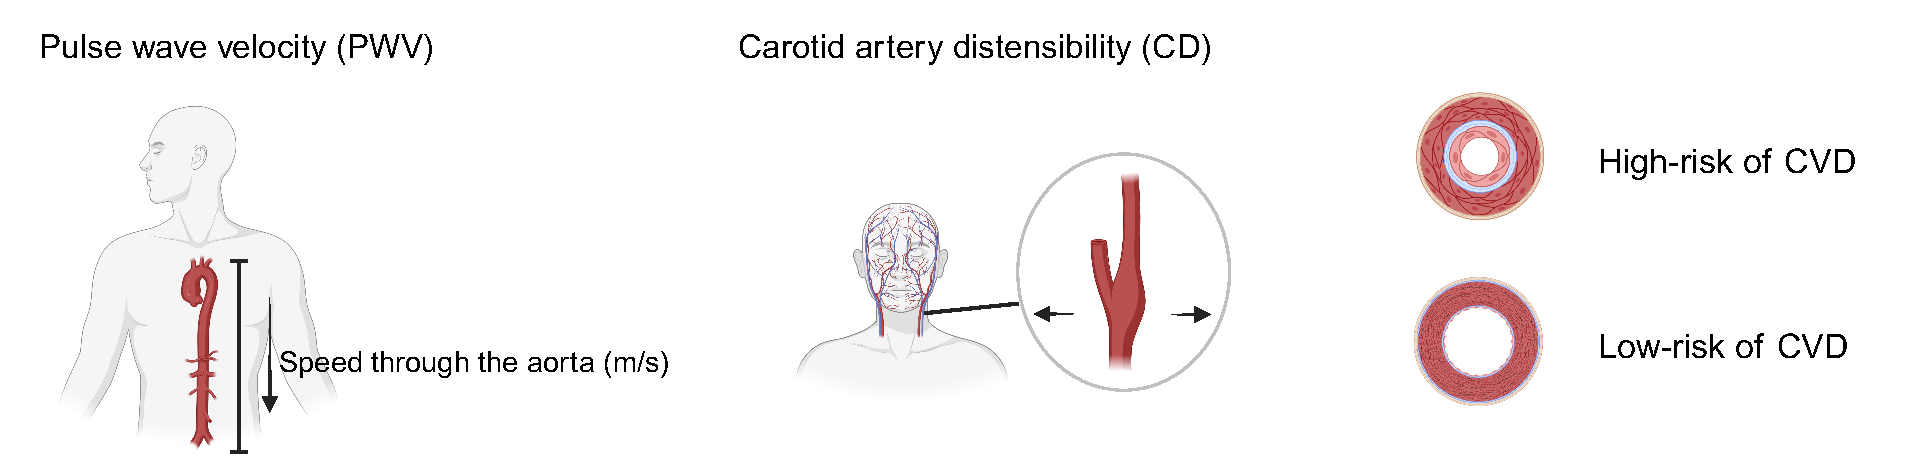
\includegraphics{images/Methods_arterial_stiffness.pdf} \emph{Measures
of arterial stiffness, measured dynamically through the decending aorta
and locally ay carotid sites. (Source: Author)}

}

\caption{\label{fig-as}\textbf{Aortic and carotid stiffness}}

\end{figure}

\hypertarget{indicators-of-heart-failure}{%
\subsection{Indicators of heart
failure}\label{indicators-of-heart-failure}}

N-terminal prohormone of brain natriuretic peptide (NT-proBNP) is a
natriuretic peptide that can be used to detect patients with heart
failure and monitor its progression. It is derived from B-type
natriuretic peptide (BNP), a cardiac neurohormone synthesized and
secreted in response to stretched cardiomyocytes and cardiac volume
overload. After secretion, proBNP is cleaved, releasing the active
hormone BNP along with the remaining N-terminal fragment, known as
NT-proBNP. In Study III, a blood sample was taken at the study site. A
description of the NT-proBNP analysis of plasma samples is provided in
the supplementary material in Appendix Study III.\textsuperscript{88}

A modified version of the validated WATCH-DM heart failure risk score
was used. The risk score is based on nine variables: two binary (history
of myocardial infarction and coronary artery bypass grafting) and seven
continuous (age, BMI, systolic/diastolic BP, serum creatinine, HDL
cholesterol, and HbA1c). Scores range from 0--39 and are categorized as
very low (≤11), low (12--13), moderate (14--15), high (16--18), and very
high (≥19) risk.\textsuperscript{88,91,92}

NYHA class stage I--IV was included. Heart failure symptoms were defined
as NYHA class II--IV, assessed by a physician.\textsuperscript{88}

\hypertarget{cardiovascular-events}{%
\subsection{Cardiovascular events}\label{cardiovascular-events}}

Information on CVD events and mortality was obtained from the Danish
National Patient Registers until 2021 by utilizing the ICD-10 codes for
stroke, myocardial infarction, cardiovascular death, cardiovascular
revascularization, and heart failure. Three-point major adverse
cardiovascular events (MACE) was defined as myocardial infarction,
stroke, cardiovascular revascularization, and cardiovascular
death.\textsuperscript{87}

\begin{table}

\caption{\label{tbl-mace}\textbf{?(caption)}}\begin{minipage}[t]{\linewidth}
\subcaption{\label{tbl-mace-1}Definition of CVD and Heart failure}

{\centering 

\begin{tabular}[t]{ll}
\toprule
\textbf{Outcome} & \textbf{Diagnosis codes}\\
\emph{Heart failure} & ICD: I50\\
\emph{Three-point MACE} & \\
Stroke & ICD: I61 - I64\\
Myocardial infarction & ICD: I21-I24\\
Cardiovascular death & ICD: I20-I28, I42, I46\\
Cardiovascular revascularization & SKA: KPAE10, KPAE25, KPAF10, KPAF20,
KPAF21, KPAF22, KPAH10, KPAH20, KPAH21, KPEE, KPEF, KPEH, KPEP, KPEQ,
KPFE,, KPFH, KPFP, KPFQ\\
\bottomrule
\end{tabular}

}

\end{minipage}%

\end{table}

\hypertarget{statistical-methods}{%
\section{Statistical Methods}\label{statistical-methods}}

\hypertarget{cross-sectional-analysis}{%
\subsection{Cross-sectional analysis}\label{cross-sectional-analysis}}

\emph{Study I}

In Study I, multiple linear regression was used to investigate
associations between 24-hour HRV and arterial stiffness. Model 1 was
adjusted for age, sex, education, glucose metabolism status, and mean
arterial pressure (MAP) to account for the oversampling of individuals
with T2D and potential instrumental bias of arterial pressure flow.
Model 2 included additional adjustments for smoking behavior, alcohol
consumption, physical activity, BMI, HbA1c, triglycerides, total-to-HDL
cholesterol ratio, and medication use. Arterial stiffness measures were
log-transformed to ensure normally distributed residuals and were
back-transformed into percentage change estimates. A sex interaction
term was added to assess whether the association differed by sex.
Sensitivity analyses were performed excluding individuals on
antihypertensive treatment or glucose-lowering
medication.\textsuperscript{77}

\emph{Study III}

In Study III, logistic regression models were applied to investigate the
association between CAN and heart failure, using elevated NT-proBNP
(concentration \textgreater125 pg/ml) as the primary outcome.
Adjustments were made for age, sex, diabetes duration, smoking behavior,
alcohol consumption, BMI, HbA1c, triglycerides, total cholesterol,
antihypertensive medication, eGFR, and prior CVD. Sensitivity analyses
were performed excluding participants with beta-blocker treatment or
prior CVD. Logistic regression was also applied to assess the odds of
CAN being associated with heart failure symptoms, defined as NYHA class
II or higher, adjusting for covariates in the primary analysis. Linear
regression was employed to evaluate differences in the WATCH-DM risk
score between individuals with and without CAN.\textsuperscript{88}

\hypertarget{time-to-event-analysis}{%
\subsection{Time-to-event analysis}\label{time-to-event-analysis}}

In Study II, Poisson regression models were used to quantify the
associations between multiday HRV and cardiovascular events, as
follow-up data were undisturbed over time and to avoid assumptions of
proportional hazards.\textsuperscript{93} Multiday HRV was modelled
using splines with knots at predefined percentiles to assess non-linear
associations. Hourly HRV was analysed separately for each hour to
observe whether the association of HRV exhibited diurnal variation. Both
HRV and mHR were standardized by their mean and standard deviation to
ensure comparability. Based on assumptions about potential confounding
pathways summarized in directed acyclic graphs (DAGs), two models were
fitted: Model 1 adjusted for age and sex, while Model 2 further adjusted
for education, smoking, alcohol consumption, physical activity (PAEE
calculated from the Recent Physical Activity Questionnaire, RPAQ), body
mass index, total cholesterol, and HbA1c. Additional analyses were
performed with HRV pre-adjusted for concurrent heart rate and physical
acceleration to account for the influence of these factors. Missing
covariates were handled using multiple imputation. Each individual's
follow-up period began at the time of their inclusion in the baseline
examination.\textsuperscript{87}

To calculate age-specific incidence rates (IR), follow-up ended at the
earliest occurrence of CVD, heart failure, all-cause mortality, or the
end of the study period. The follow-up time was divided into one-year
intervals based on the individual's age. Using this age-split data,
incidence rates of CVD, heart failure, and all-cause mortality were
analysed in relation to HRV, with age treated as a time-varying
covariate in a Poisson regression model.

\hypertarget{effect-modification}{%
\subsection{Effect modification}\label{effect-modification}}

Effect modification was assessed to determine whether the association
between an exposure and an outcome varied depending on the level of a
third variable, known as the effect modifier.\textsuperscript{94}

In Study I, it was hypothesized that the association between 24-hour HRV
and arterial stiffness was stronger in strata of diabetes progression
(normal glucose metabolism, prediabetes, T2D). Therefore, an interaction
term between HRV and diabetes status was included to observe the size of
the association across strata.\textsuperscript{77} A subsidiary analysis
was conducted in a subpopulation without T2D to assess whether the
effect was modified by HbA1c. In Study II, the variation in the
association between multiday HRV and CVD endpoints by sex was quantified
to explore potential biological dimorphism.\textsuperscript{87} In Study
III, the presence of an association between CAN and elevated NT-proBNP
in the subgroup without symptoms (NYHA class \textless{} II) was
examined. It was hypothesized that no significant effect modification
would be observed between groups with and without symptoms. Similarly,
the persistence of the association in the group classified as low to
moderate risk of heart failure was explored, based on the WATCH-DM risk
score.\textsuperscript{88}

A significant effect modification was defined as an interaction term
with a p-value \textless{} 0.05.

\hypertarget{multiple-imputed-by-chained-equations}{%
\subsection{Multiple imputed by chained
equations}\label{multiple-imputed-by-chained-equations}}

Multiple Imputation by Chained Equations (MICE) was used to handle
missing data. This procedure imputes missing values through an iterative
series of predictive models, generating plausible estimates while
preserving the relationships within the data. To avoid assigning the
same confidence to imputed values as to observed values, Rubin's rules
were followed. Rubin's rules combine results from multiple imputed
datasets by pooling estimates of interest (e.g., means or regression
coefficients) using their within- and between-imputation
variances.\textsuperscript{95} This approach ensures valid statistical
inferences by accounting for the uncertainty introduced by missing data.

In Study II, confounders were imputed to include as many participants as
possible and to avoid excluding individuals with or without
cardiovascular or mortality events. The dataset was imputed 10 times. In
Study III, missing CARTs were imputed, as a proportion of participants
had non-valid tests due to insufficient air in the Valsalva manoeuvre,
unstable heartbeats, or data errors. These variables were used as
auxiliary variables in the imputation to reduce
bias.\textsuperscript{96} All available variables on biochemical
measures, diagnoses, medications, and causes of non-valid CARTs were
used to impute each missing CART using predictive mean
matching.\textsuperscript{88}

\hypertarget{instrumental-bias}{%
\subsection{Instrumental bias}\label{instrumental-bias}}

In Studies I--III, physiological properties were investigated using
dynamic measures and biomarkers to quantify autonomic function, arterial
stiffness, and cardiac function. Other conditions may influence the
properties being measured, thereby introducing instrumental bias.

\emph{Vascular Stiffness}

In Study I, arterial stiffness was measured using cf-PWV and carotid
distensibility. Both measures are influenced by arterial pressure at the
time of examination. Arterial pressure affects the propagation of the
pressure wave through the aorta (cf-PWV) and the expansion and
contraction of the carotid artery (carotid
distensibility).\textsuperscript{97} To account for this, adjustments
were made for MAP in the models.\textsuperscript{77}

\emph{Cardiovascular autonomic function}

In Study II, autonomic function was assessed using multiday HRV
recordings and hourly HRV measurements. Previous studies have shown that
HRV is dependent on heart rate, and low HRV may simply reflect a higher
resting heart rate (rHR). To adjust for this without overcorrecting for
a collinear variable, HRV was pre-adjusted by regressing rHR on HRV,
extracting the residuals, and using these as the pre-adjusted
determinant. For hourly HRV, variability in heart rate may be influenced
by changes in physical activity, creating a risk that HRV serves as a
proxy for movement rather than autonomic function. To address this, a
similar pre-adjustment approach was applied by regressing concurrent
heart rate and physical acceleration to account for physical
activity.\textsuperscript{87}

\emph{Biomarker of Heart Failure}

In Study III, kidney function and overweight are known to influence
NT-proBNP levels independently of heart failure.\textsuperscript{58} The
model was adjusted to account for the confounding effect of eGFR on
NT-proBNP levels in the analysis.\textsuperscript{88}

\clearpage
\null
\thispagestyle{empty}
\clearpage

\bookmarksetup{startatroot}

\hypertarget{results}{%
\chapter{Results}\label{results}}

\clearpage
\null
\thispagestyle{empty}
\clearpage

In this section, study population characteristics and findings from
analysis will be presented.

\hypertarget{study-i}{%
\section{Study I}\label{study-i}}

\hypertarget{descriptive}{%
\subsection{Descriptive}\label{descriptive}}

In The Maastricht Study, 7,449 participants were included between
November 2010 and December 2020, of whom 1,316 reported a history of
CVD.\textsuperscript{77} A total of 4,379 participants had valid 24-hour
HRV measurements, and among these, 3,673 had a valid measurement of
either CD or cf-PWV. Study population included 3673 participants. The
study population represented diabetes risk of NGM (65\%), prediabetes
(15\%), and T2D (20\%). The median (IQR) cf-PWV (aortic stiffness)
became higher with diabetes status: NGM: 8.08 m/s (7.28, 9.16),
prediabetes: 8.96 m/s (7.84, 10.32), and T2D: 9.36 m/s (8.16, 10.80). CD
(carotid stiffness) decreased: NGM: 15.0 (11.8, 18.8), prediabetes: 13.5
(10.4, 16.9), and T2D: 12.5 (9.9, 16.0) × 10⁻³/kPa. SDNN (ms) was
highest in NGM and lowered with worsening glucose metabolism: NGM: 138ms
(117, 164), prediabetes: 127ms (106, 152), and T2D: 116ms (96, 139).
Further description of characteristics by diabetes are described in
Table~\ref{tbl-ms}.

\newgeometry{top=2cm, bottom=2cm, inner=0.2cm, outer=0.2cm}

\hypertarget{tbl-ms}{}
\begin{landscape}\begin{table}
\caption{\label{tbl-ms}Study charteristics in The Maastricht Study (Study I) by diabetes status }\tabularnewline

\centering\begingroup\fontsize{10}{12}\selectfont

\resizebox{\linewidth}{!}{
\begin{tabular}[t]{llll}
\toprule
Characteristic & Normal glucose metabolism
N = 2,389 & Prediabetes  
N = 538 & Type 2 Diabetes  
N = 746\\
\midrule
\cellcolor{gray!6}{Women} & \cellcolor{gray!6}{1,361 (57\%)} & \cellcolor{gray!6}{258 (48\%)} & \cellcolor{gray!6}{265 (36\%)}\\
Age (years) & 58 (51, 64) & 62 (57, 68) & 63 (57, 68)\\
\cellcolor{gray!6}{Moderate to vigorous physical activity (hours/week)} & \cellcolor{gray!6}{5.3 (3.0, 8.3)} & \cellcolor{gray!6}{4.5 (2.3, 7.5)} & \cellcolor{gray!6}{3.8 (1.5, 6.8)}\\
BMI (kg/m²) & 25.0 (22.9, 27.4) & 27.2 (24.9, 30.1) & 28.8 (26.0, 31.7)\\
\cellcolor{gray!6}{HbA1c (\%)} & \cellcolor{gray!6}{5.35 (5.17, 5.63)} & \cellcolor{gray!6}{5.63 (5.35, 5.90)} & \cellcolor{gray!6}{6.54 (6.08, 7.09)}\\
\addlinespace
HDL (mmol/L) & 1.60 (1.30, 2.00) & 1.40 (1.20, 1.80) & 1.30 (1.00, 1.50)\\
\cellcolor{gray!6}{Total cholesterol (mmol/L)} & \cellcolor{gray!6}{5.50 (4.80, 6.20)} & \cellcolor{gray!6}{5.50 (4.80, 6.30)} & \cellcolor{gray!6}{4.50 (3.90, 5.20)}\\
Triglycerides (mmol/L) & 1.05 (0.80, 1.45) & 1.39 (1.03, 1.90) & 1.51 (1.08, 2.14)\\
\cellcolor{gray!6}{Duration of type-2 diabetes (only for diagnosed participants)} & \cellcolor{gray!6}{} & \cellcolor{gray!6}{} & \cellcolor{gray!6}{3 (0, 9)}\\
Mean IBI (ms) & 838 (775, 907) & 815 (760, 897) & 806 (744, 889)\\
\addlinespace
\cellcolor{gray!6}{SDNN (ms)} & \cellcolor{gray!6}{138 (117, 164)} & \cellcolor{gray!6}{127 (106, 152)} & \cellcolor{gray!6}{116 (96, 139)}\\
RMSSD (ms) & 26 (21, 34) & 24 (19, 33) & 22 (17, 31)\\
\cellcolor{gray!6}{TP (ms²)} & \cellcolor{gray!6}{12,596 (8,880, 17,498)} & \cellcolor{gray!6}{10,615 (7,134, 15,374)} & \cellcolor{gray!6}{8,880 (6,064, 12,722)}\\
ULF (ms²) & 10,771 (7,392, 15,142) & 8,948 (5,852, 13,374) & 7,524 (5,036, 11,001)\\
\cellcolor{gray!6}{VLF (ms²)} & \cellcolor{gray!6}{1,198 (833, 1,692)} & \cellcolor{gray!6}{1,015 (685, 1,478)} & \cellcolor{gray!6}{816 (541, 1,267)}\\
\addlinespace
HF (ms²) & 94 (57, 158) & 78 (47, 138) & 63 (36, 117)\\
\cellcolor{gray!6}{Systolic blood pressure (mmHg)} & \cellcolor{gray!6}{123 (114, 133)} & \cellcolor{gray!6}{129 (122, 140)} & \cellcolor{gray!6}{130 (122, 139)}\\
Diastolic blood pressure (mmHg) & 75 (71, 80) & 78 (73, 83) & 76 (72, 81)\\
\cellcolor{gray!6}{Mean arterial pressure (mmHg)} & \cellcolor{gray!6}{95 (88, 102)} & \cellcolor{gray!6}{99 (93, 107)} & \cellcolor{gray!6}{98 (92, 105)}\\
Carotid artery distensibility (10-3/kPa) & 15.0 (11.8, 18.8) & 13.5 (10.4, 16.9) & 12.5 (9.9, 16.0)\\
\addlinespace
\cellcolor{gray!6}{Carotid-femoral pulse wave velocity (m/s)} & \cellcolor{gray!6}{8.08 (7.28, 9.16)} & \cellcolor{gray!6}{8.96 (7.84, 10.32)} & \cellcolor{gray!6}{9.36 (8.16, 10.80)}\\
Glucose-lowering medication & 0 (0\%) & 0 (0\%) & 519 (70\%)\\
\cellcolor{gray!6}{Antihypertensive medication} & \cellcolor{gray!6}{431 (18\%)} & \cellcolor{gray!6}{199 (37\%)} & \cellcolor{gray!6}{478 (64\%)}\\
Beta blockers & 149 (6.2\%) & 77 (14\%) & 195 (26\%)\\
\cellcolor{gray!6}{Lipid-lowering medication} & \cellcolor{gray!6}{280 (12\%)} & \cellcolor{gray!6}{141 (26\%)} & \cellcolor{gray!6}{484 (65\%)}\\
\bottomrule
\multicolumn{4}{l}{\rule{0pt}{1em}\textit{Note: }}\\
\multicolumn{4}{l}{\rule{0pt}{1em}makecell[l]{Categorical variables: N (\%); Continous variables: Median (IQT:25th-75th)\    Table are adapted from supplementary material in Appendix Study I}}\\
\end{tabular}}
\endgroup{}
\end{table}
\end{landscape}

\restoregeometry

\hypertarget{hour-hrv-and-arterial-stiffness}{%
\subsection{24-hour HRV and arterial
stiffness}\label{hour-hrv-and-arterial-stiffness}}

\textbf{Time-domain HRV}

In the fully adjusted model 2, cf-PWV was 2.8\% (CI: 2.1; 3.4) lower,
while CD was 3.3\% (CI: 1.5; 5.1) higher per SD higher in HRV
time-domain Z-score (see see Figure~\ref{fig-MS-HRV} A and B). Among the
time-domain indices, SDNN, SDNNi, and SDANN showed the strongest
associations, with cf-PWV being lower by 2.5\% (CI: 2.0; 3.1), 2.5\%
(CI: 1.9; 3.4), and 2.2\% (CI: 1.7; 2.7),
respectively.\textsuperscript{77} Conversely, CD was higher by 3.2\%
(CI: 1.7; 4.7), 3.0 \% (CI: 1.4; 4.6), and 2.8\% (CI: 1.3; 4.3),
respectively. RMSSD and pNN50 showed a weaker association with cf-PWV
(-1.1\% {[}CI: -1.4; -0.4{]}, and -1.1 {[}-1.7; -0.6{]}), while no
evidence for an association was found with CD.\textsuperscript{77}

\textbf{Frequency-domain HRV}

In the fully adjusted model 2, cf-PWV was 2.8\% (CI: 2.1; 3.5) lower,
while CD was 3.2\% (CI: 1.3; 5.1) higher per SD higher in HRV
frequency-domain Z-score (see see Figure~\ref{fig-MS-HRV} C and D).
Among the frequency-domain indices, total power, VLF, and ULF showed the
strongest associations, with cf-PWV being lower by 2.2\% (CI: 1.7; 2.8
), 2.4\% (CI: 1.9; 4.0), and 2.1\% (CI: 1.5; 2.6),
respectively.\textsuperscript{77} Conversely, CD was higher by 2.7\%
(CI: 1.2; 4.2), 2.4\% (CI: 0.9; 4.1), and 2.6\% (CI: 1.1; 4.1),
respectively. HF showed a weaker association with cf-PWV (-0.9\% {[}CI:
-1.4; -0.4{]}), while no evidence for an association was found with CD.
Mean interbeat interval was associated with 2.4 \% (CI: 1.8; 2.9) lower
cf-PWV and 4.5\% (3.1; 6.1) higher CD.\textsuperscript{77}

\begin{figure}

{\centering 

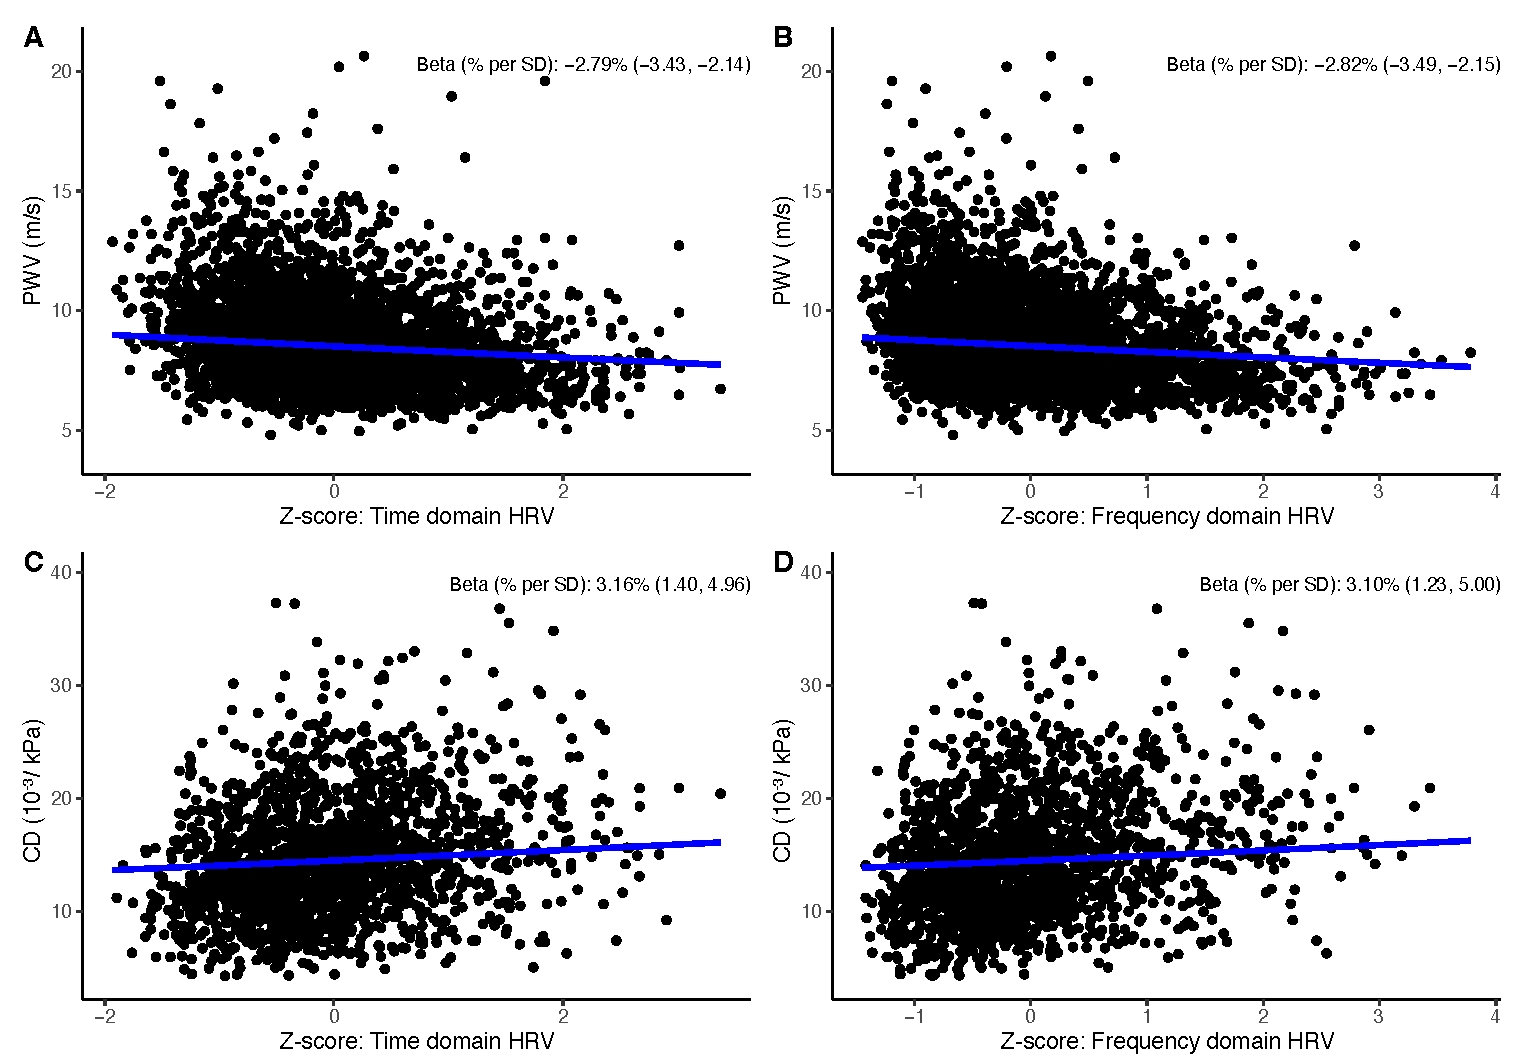
\includegraphics{images/figure3_linear_plot.pdf}

\emph{A: Percentage PWV per SD in time-domain composite z-score B:
Percentage PWV per SD in frequency-domain composite z-score C:
Percentage higher CD per SD in time-domain composite z-score D:
Percentage CD per SD in frequency-domain composite z-score. All
regression lines were adjusted for being a male, 60 years old, low
educational level, without prediabetes or type-2 diabetes, and with
96mmHg MAP. From Figure 1 in Appendix Study I\textsuperscript{77}}

}

\caption{\label{fig-MS-HRV}\textbf{Association between HRV and arterial
stiffness}}

\end{figure}

\hypertarget{effect-modification-of-diabetes-status}{%
\subsection{Effect modification of diabetes
status}\label{effect-modification-of-diabetes-status}}

The association between HRV time-domain Z-scores and cf-PWV and CD was
significantly modified by prediabetes (cf-PWV: -4.9 {[}CI: -6.5; -3.2{]}
\(^{interaction(*) ^{p-value< 0.01}}\) CD: 8.0 {[}CI:3.8;
12.5{]}\(^{*^{p-value< 0.01}}\)) but not by T2D (cf-PWV: -3.5 \% {[}CI:
-4.8; -2.1){]} \(^{*^{p-value< 0.1}}\) CD: 4.8 \% {[}CI:1.3;
8.4{]}\(^{*^{p-value< 0.1}}\))\textsuperscript{77}. For the indices SDNN
and SDANN, the association with both cf-PWV and CD was significantly
modified by both prediabetes and T2D\textsuperscript{77}.

The association between HRV frequency-domain Z-score and cf-PWV was
statistically significant modified from NGM by prediabetes (-5.7
\%{[}CI:-7.4; -3.9{]}\(^{*^{p-value< 0.01}}\)) and T2D (-3.9
\%{[}CI:-5.4; -2.3{]}\(^{*^{p-value< 0.05}}\)) while CD was only
modified by prediabetes (8.3 \%{[}CI:3.6;
13.2{]}\(^{*^{p-value< 0.01}}\)) but not by T2D (5.3 \%{[}CI:1.4;
9.4{]}\(^{*^{p-value< 0.1}}\))\textsuperscript{77}. For the indices
total power and ULF, the association with both cf-PWV and CD was
statistically significant modified by both prediabetes and T2D. Mean
inter beat interval association with cf-PWV or CD was not significantly
modified by diabetes status\textsuperscript{77}.

As no stepwise increase was observed in the modification of glucose
metabolism status from prediabetes to T2D,the subgroup with T2D was
excluded to test whether the association was gradually modified by
dysglycemia. In this subgroup, the association between HRV time and
frequency-domain Z-scores and measures of arterial stiffness was
modified by HbA1c (range of interaction p-values: 0.1 to 0.005) (see
Figure Figure~\ref{fig-MS-HRV}). For example, per SD lower HRV frequency
domain Z-score at HbA1c 6.4\% was associated with a 5.4\% higher (CI:
3.5; 7.2) cf-PWV, which was 2.0\% to 4.0\% higher compared to the
magnitude of association at HbA1c levels of 5.6\% and 4.8\% (see see
Figure~\ref{fig-MS-HRV} B). In CD, per SD lower HRV frequency domain
Z-score at HbA1c 6.4\% was associated with an 8.1\% lower (CI: -13.5;
-2.9) CD, which was 4.8\% to 9.5\% lower compared to the magnitude of
association at HbA1c levels of 5.6\% and 4.8\% (see
Figure~\ref{fig-MS-HRV} D). No association between HRV frequency domain
Z-score and CD was observed at HbA1c levels between 4.8\% and 5.2\%.

\newgeometry{top=2cm, bottom=2cm, inner=0.5cm, outer=0.5cm}

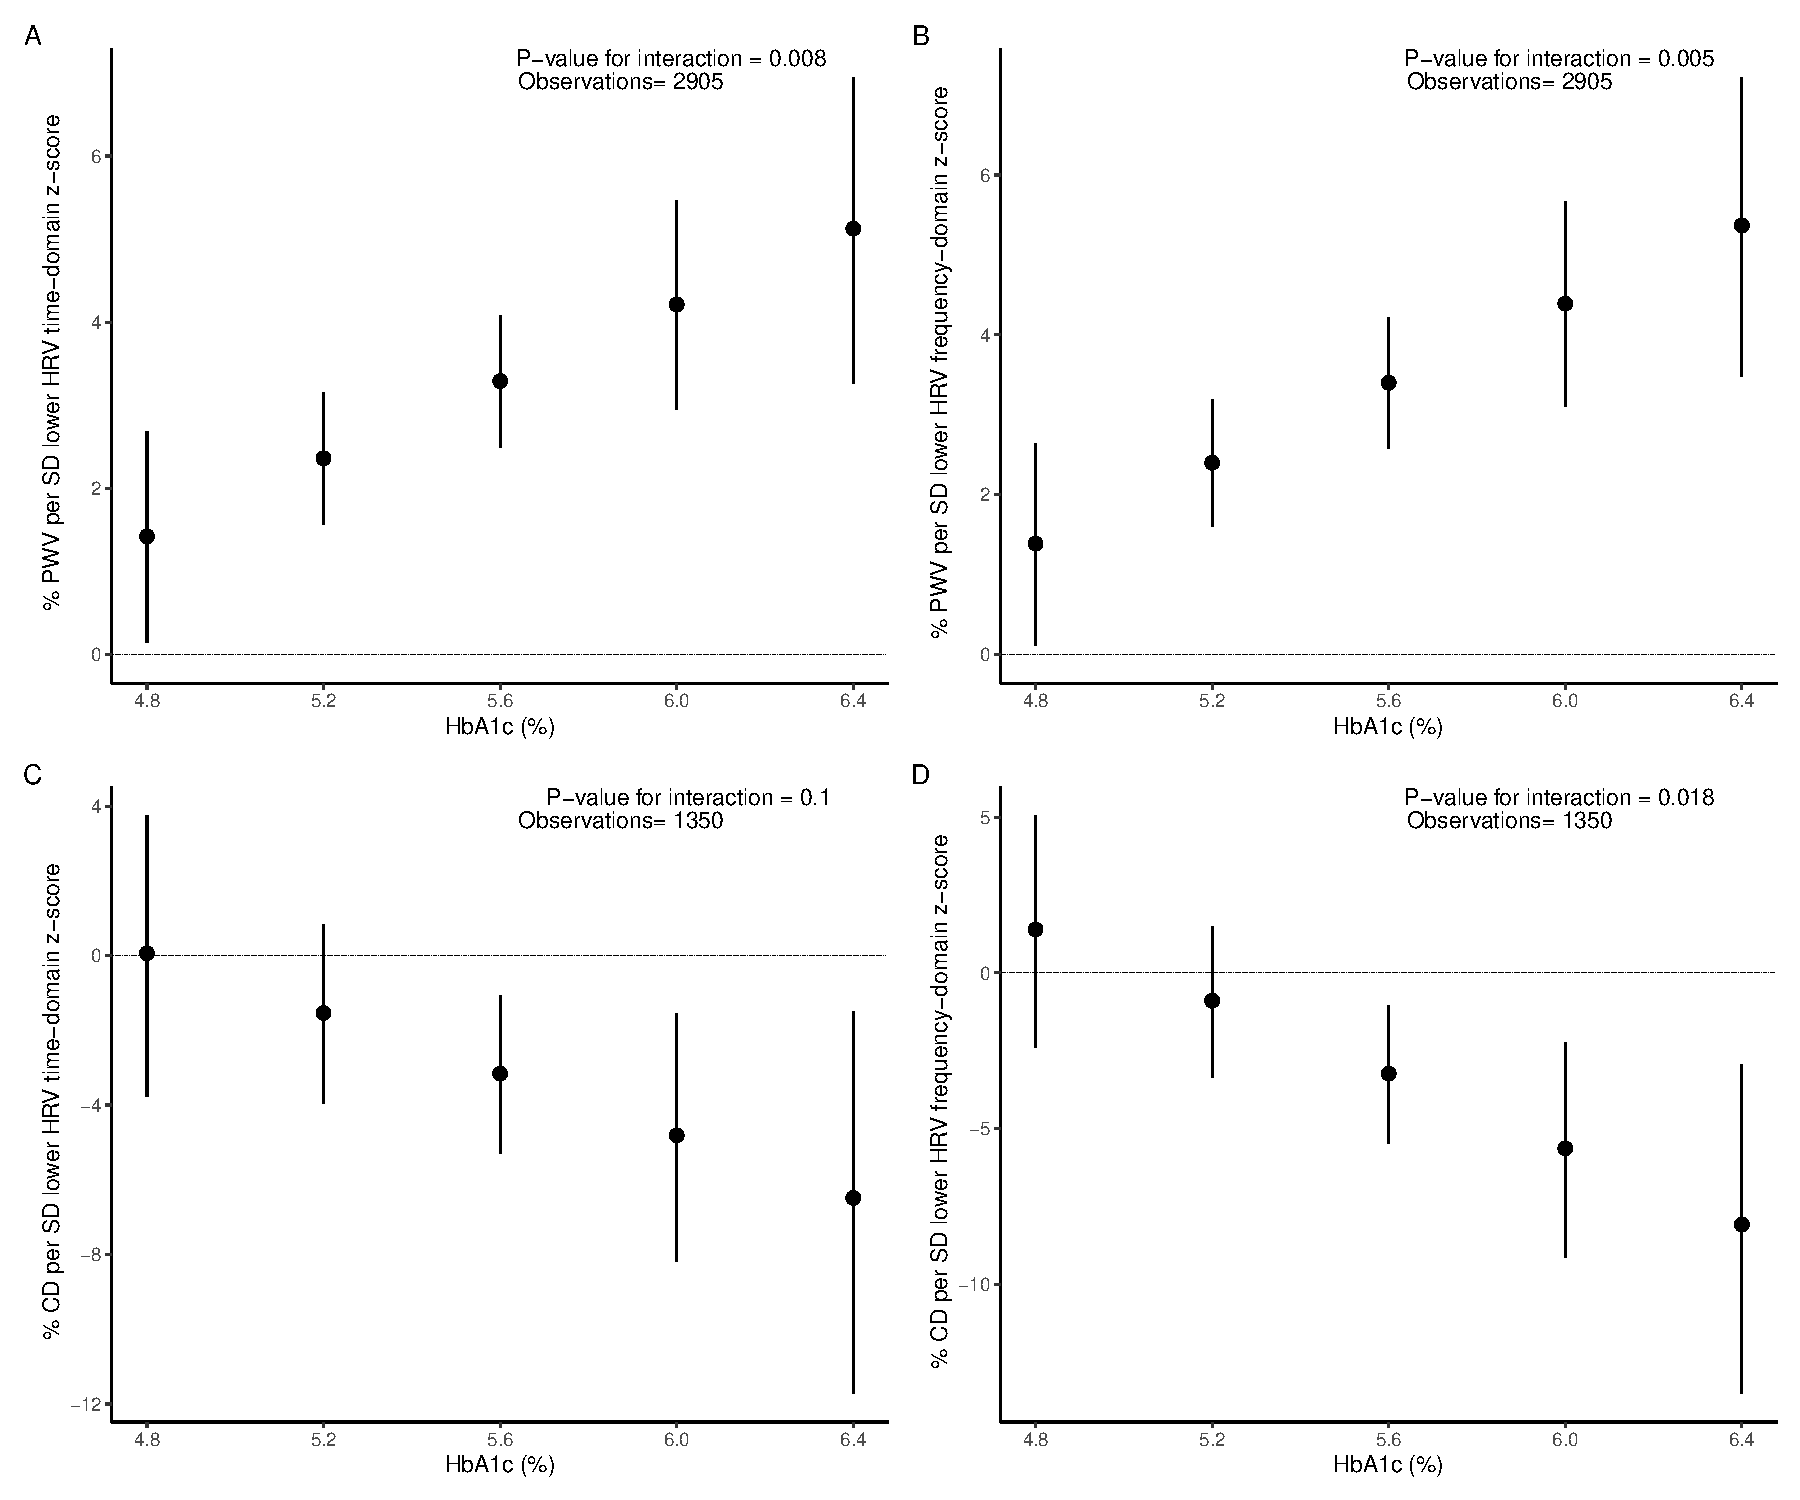
\includegraphics{images/em_hba1c.pdf}

\emph{A: Percentage PWV per SD in time-domain composite z-score B:
Percentage PWV per SD in frequency-domain composite z-score C:
Percentage higher CD per SD in time-domain composite z-score D:
Percentage CD per SD in frequency-domain composite z-score. Model
adjusted for sex, age, educational status, diabetes status, and MAP,
physical activity, smoking behaviour, alcohol use, body mass index,
hba1c, triglycerides, total-to-high density lipoprotein cholesterol
ratio, lipid-modifying- and antihypertensive medication. Figure was
based on data in Study I\textsuperscript{77}}

\restoregeometry

\hypertarget{study-ii}{%
\section{Study II}\label{study-ii}}

\hypertarget{descriptive-1}{%
\subsection{Descriptive}\label{descriptive-1}}

The ADDITION-PRO population consisted of 1,627 participants with at
least 48-hour HRV measures, while 1,432 had all hours represented with
hourly HRV and physical acceleration. The study population included
different tiers of diabetes risk: 154 individuals at low risk (9\%), 889
at high risk (51\%), 314 with impaired fasting glucose (IFG) (18\%), 226
with impaired glucose tolerance (IGT) (13\%), and 161 with both IFG and
IGT (9\%). SDNN was categorized into five groups: very-low
(SDNN\textless{} 100 ms), low (SDNN 100-120 ms), middle (SDNN 121-140
ms), high (SDNN 141-160 ms) and very-high (SDNN \textgreater160 ms).

Characteristics are described in Table~\ref{tbl-add}. Participants in
the lowest SDNN group (\textless100 ms) were older (67.4 ± 6.9 years),
had higher BMI (28.1 ± 5.4), HbA1c (5.9 ± 0.9), triglycerides (1.5 ± 0.9
mmol/L), and rHR (67.8 ± 5.7 bpm), were more likely to use
anti-hypertensive medication (61\%), and had lower physical activity
energy expenditure (46.8 ± 24.0 kJ/day) compared to those with higher
SDNN levels.

\newgeometry{top=2cm, bottom=2cm, inner=0.5cm, outer=0.5cm}

\hypertarget{tbl-add}{}
\begin{landscape}\begin{table}
\caption{\label{tbl-add}Study characteristics in The ADDITION-PRO Study (Study II) by SDNN
categories }\tabularnewline

\centering\begingroup\fontsize{10}{12}\selectfont

\resizebox{\linewidth}{!}{
\begin{tabular}[t]{lllllll}
\toprule
SDNN Categories & Overall, N = 1,625
 & <100 ms, N = 148
 & 100-120 ms, N = 312
 & 120-140 ms, N = 457
 & 140-160 ms, N = 346
 & >160 ms, N = 362
\\
\midrule
\cellcolor{gray!6}{Women} & \cellcolor{gray!6}{759 (47\%)} & \cellcolor{gray!6}{80 (54\%)} & \cellcolor{gray!6}{164 (53\%)} & \cellcolor{gray!6}{251 (55\%)} & \cellcolor{gray!6}{143 (41\%)} & \cellcolor{gray!6}{121 (33\%)}\\
Age (years) & 65.9 (6.8) & 67.4 (6.9) & 65.7 (6.9) & 66.0 (6.7) & 65.5 (6.6) & 66.0 (7.0)\\
\cellcolor{gray!6}{Physical activity energy expenditure (KJ / day)} & \cellcolor{gray!6}{53.1 (25.1)} & \cellcolor{gray!6}{46.8 (24.0)} & \cellcolor{gray!6}{49.4 (21.0)} & \cellcolor{gray!6}{50.7 (21.5)} & \cellcolor{gray!6}{57.6 (27.2)} & \cellcolor{gray!6}{57.5 (29.2)}\\
Alcohol consumption (units per week) & 9.2 (9.5) & 11.3 (10.8) & 10.2 (11.3) & 8.9 (8.5) & 8.5 (9.2) & 8.7 (8.2)\\
\cellcolor{gray!6}{Smoking status} & \cellcolor{gray!6}{} & \cellcolor{gray!6}{} & \cellcolor{gray!6}{} & \cellcolor{gray!6}{} & \cellcolor{gray!6}{} & \cellcolor{gray!6}{}\\
\addlinespace
Current & 263 (16\%) & 40 (28\%) & 70 (23\%) & 65 (14\%) & 41 (12\%) & 47 (13\%)\\
\cellcolor{gray!6}{Prior} & \cellcolor{gray!6}{750 (47\%)} & \cellcolor{gray!6}{58 (40\%)} & \cellcolor{gray!6}{145 (47\%)} & \cellcolor{gray!6}{214 (47\%)} & \cellcolor{gray!6}{162 (47\%)} & \cellcolor{gray!6}{171 (48\%)}\\
Never & 598 (37\%) & 47 (32\%) & 95 (31\%) & 174 (38\%) & 140 (41\%) & 142 (39\%)\\
\cellcolor{gray!6}{BMI (kg/m²)} & \cellcolor{gray!6}{27.7 (4.7)} & \cellcolor{gray!6}{28.1 (5.4)} & \cellcolor{gray!6}{28.2 (4.6)} & \cellcolor{gray!6}{28.0 (4.7)} & \cellcolor{gray!6}{27.7 (4.9)} & \cellcolor{gray!6}{26.9 (4.2)}\\
Waist circumference (cm) & 96.7 (13.4) & 98.0 (14.9) & 98.2 (13.2) & 96.7 (13.6) & 96.7 (13.1) & 94.8 (12.5)\\
\addlinespace
\cellcolor{gray!6}{Systolic blood pressure (mmHg)} & \cellcolor{gray!6}{133.7 (17.3)} & \cellcolor{gray!6}{134.2 (16.3)} & \cellcolor{gray!6}{133.7 (17.6)} & \cellcolor{gray!6}{133.5 (17.8)} & \cellcolor{gray!6}{133.4 (16.9)} & \cellcolor{gray!6}{133.8 (17.5)}\\
Diastolic blood pressure (mmHg) & 81.9 (10.4) & 83.8 (10.1) & 82.7 (10.2) & 81.7 (10.6) & 82.1 (10.2) & 80.6 (10.3)\\
\cellcolor{gray!6}{HbA1c (\%)} & \cellcolor{gray!6}{5.8 (0.5)} & \cellcolor{gray!6}{5.9 (0.9)} & \cellcolor{gray!6}{5.9 (0.6)} & \cellcolor{gray!6}{5.8 (0.5)} & \cellcolor{gray!6}{5.7 (0.4)} & \cellcolor{gray!6}{5.7 (0.4)}\\
Triglycerides (mmol/L) & 1.3 (0.7) & 1.5 (0.9) & 1.4 (0.7) & 1.3 (0.6) & 1.2 (0.7) & 1.1 (0.6)\\
\cellcolor{gray!6}{Total cholesterol (mmol/L)} & \cellcolor{gray!6}{5.4 (1.1)} & \cellcolor{gray!6}{5.2 (1.0)} & \cellcolor{gray!6}{5.4 (1.2)} & \cellcolor{gray!6}{5.4 (1.1)} & \cellcolor{gray!6}{5.4 (1.0)} & \cellcolor{gray!6}{5.4 (1.0)}\\
\addlinespace
HDL cholesterol (mmol/L) & 1.6 (0.4) & 1.6 (0.4) & 1.5 (0.5) & 1.6 (0.4) & 1.6 (0.4) & 1.6 (0.4)\\
\cellcolor{gray!6}{LDL cholesterol (mmol/L)} & \cellcolor{gray!6}{3.2 (1.0)} & \cellcolor{gray!6}{3.0 (1.0)} & \cellcolor{gray!6}{3.2 (1.1)} & \cellcolor{gray!6}{3.2 (1.0)} & \cellcolor{gray!6}{3.3 (0.9)} & \cellcolor{gray!6}{3.3 (0.9)}\\
Urine albumin-creatine ratio (mg/g) & 25.9 (132.8) & 36.4 (105.9) & 47.9 (275.1) & 19.6 (48.2) & 19.4 (67.7) & 16.4 (36.3)\\
\cellcolor{gray!6}{VO2 max (mL/kg/min)} & \cellcolor{gray!6}{26.6 (7.8)} & \cellcolor{gray!6}{24.8 (7.5)} & \cellcolor{gray!6}{24.8 (7.5)} & \cellcolor{gray!6}{26.1 (6.8)} & \cellcolor{gray!6}{27.0 (8.0)} & \cellcolor{gray!6}{28.7 (8.7)}\\
Resting heart rate (bpm) & 57.3 (7.3) & 67.8 (5.7) & 63.3 (5.0) & 58.4 (4.5) & 55.0 (4.2) & 49.8 (4.9)\\
\addlinespace
\cellcolor{gray!6}{Anti-hypertensive medication (yes)} & \cellcolor{gray!6}{753 (47\%)} & \cellcolor{gray!6}{88 (61\%)} & \cellcolor{gray!6}{149 (48\%)} & \cellcolor{gray!6}{216 (47\%)} & \cellcolor{gray!6}{147 (43\%)} & \cellcolor{gray!6}{153 (43\%)}\\
\bottomrule
\multicolumn{7}{l}{\rule{0pt}{1em}\textit{Note: }}\\
\multicolumn{7}{l}{\rule{0pt}{1em}makecell[l]{Categorical variables: N (\%); Continous variables: Median (IQT:25th-75th\                         Table are based on data from Study II}}\\
\end{tabular}}
\endgroup{}
\end{table}
\end{landscape}

\restoregeometry

\hypertarget{multiday-hrv-and-mace-heart-failure-and-all-cause-mortality.}{%
\subsection{Multiday HRV and MACE, heart failure, and all-cause
mortality.}\label{multiday-hrv-and-mace-heart-failure-and-all-cause-mortality.}}

The mean multiday SDNN was 139.0 (32.3) ms, and the mean heart rate was
73.5 (9.1) bpm.\textsuperscript{87} In the fully adjusted model, SDNN
per SD was associated with a lower incidence rate ratio (IRR) for MACE
0.82 (CI: 0.69; 0.97), heart failure 0.76 (CI: 0.58; 0.99), and
mortality rate ratio of 0.79 (CI: 0.66; 0.94).\textsuperscript{87} In
model with pre-adjustment for rHR, the proportion of the association
explained between HRV and MACE, HF, and all-cause mortality was 14\%,
25\%, and 19\%, respectively.\textsuperscript{87} When knots were
included in the model, the risk was found to be higher as SDNN dropped
below approximately 120--110 ms (around the 20th percentile), suggesting
a potential threshold for elevated risk.\textsuperscript{87} Therefore,
age-specific IR were calculated at SDNN levels of 100 ms, 120 ms, and
160 ms, respectively.

\newgeometry{top=2cm, bottom=2cm, inner=0.5cm, outer=0.5cm}

\begin{figure}

{\centering 

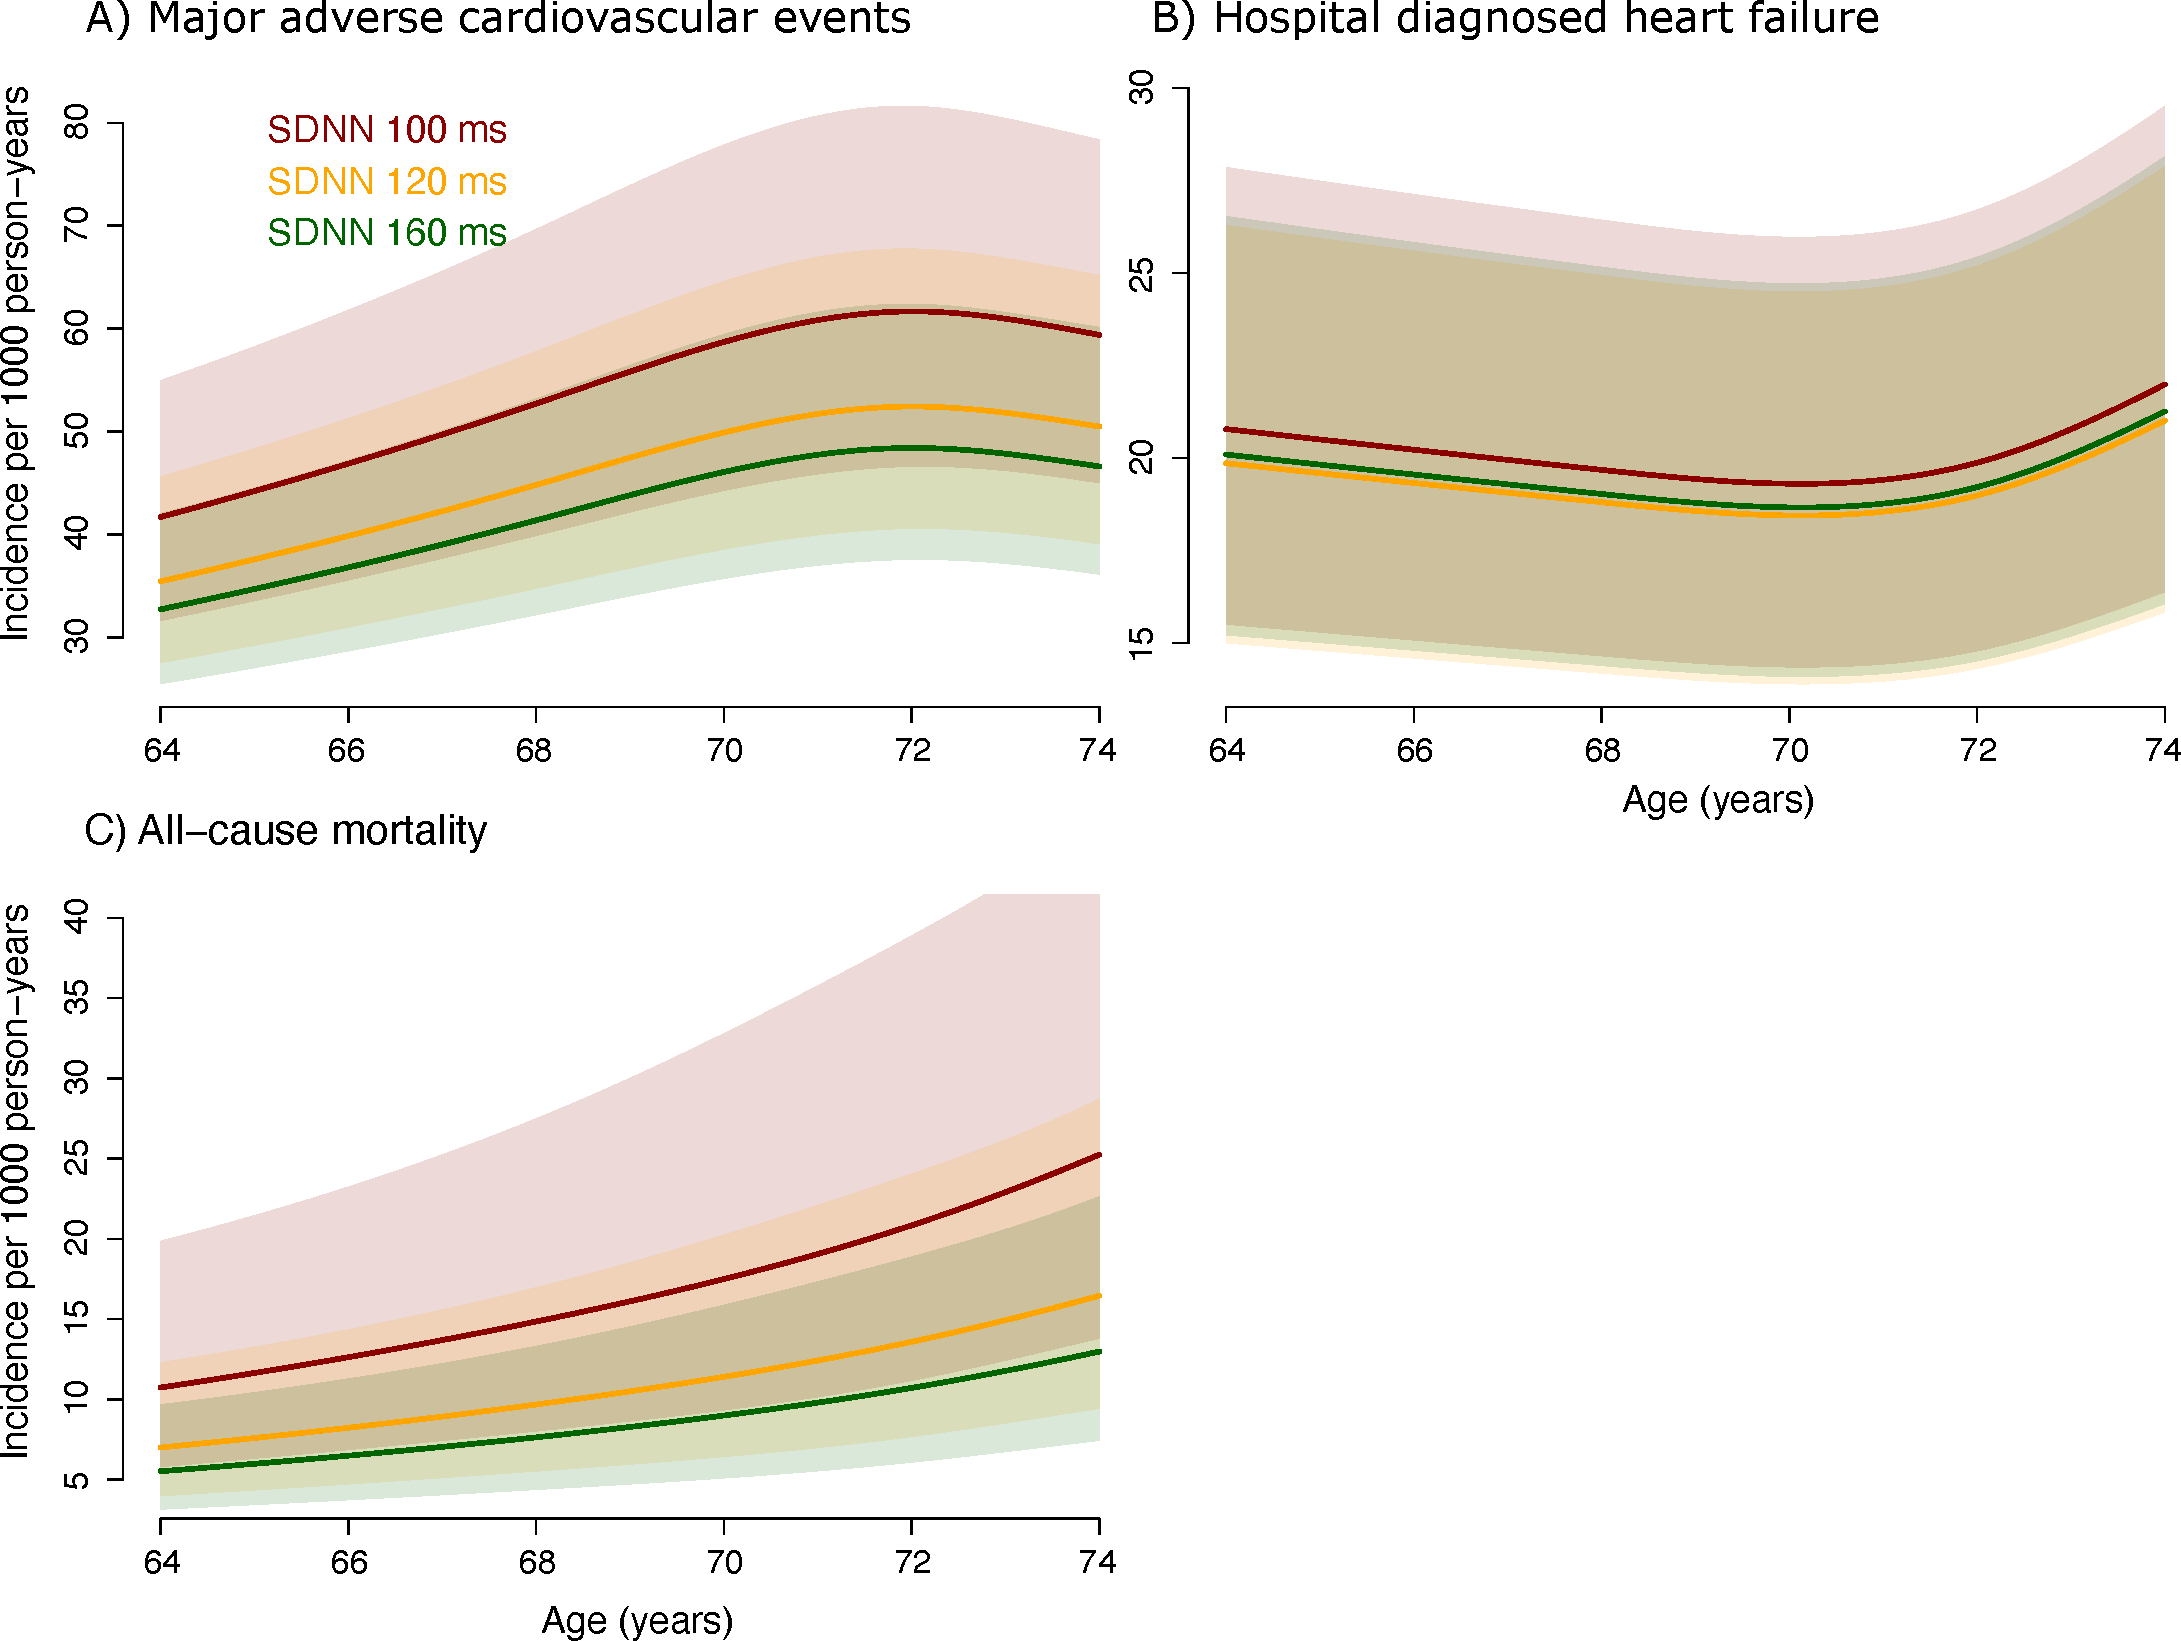
\includegraphics{images/addition_pro_hrv_ir_mace.pdf}

\emph{Multiday SDNN levels (100 ms, 120 ms, 160 ms) by age-specific
incidence rates for A) major adverse cardiovascular events, B) heart
failure hospitalisation, and C) all-cause mortality. Model adjusted for
age, sex, education, alcohol consumption, smoking behavior, physical
activity, body mass index, total cholesterol, and Hba1c. Figure was
based on data in Study II\textsuperscript{87}}

}

\caption{\label{fig-addprohrv}\textbf{Multiday SDNN and mean HR
association with major adverse cardiovascular events, heart failure, and
all-cause mortality}}

\end{figure}

\restoregeometry

At age 65, the IR per 1000 person-years for MACE was 44.2 (CI: 33.5;
58.3) at SDNN = 100 ms, which was higher than the rates observed at SDNN
= 120 ms (IR: 37.6 {[}CI: 29.2; 48.3{]}) and SDNN = 160 ms (IR: 34.7
{[}CI: 27.0; 44.5{]}) (Figure~\ref{fig-addprohrv} A). The IR was
observed to become higher with age, reaching its peak at age 72. For
heart failure at age 65, the IR was 20.5 (CI: 15.3; 27.5) at SDNN = 100
ms, slightly higher than at SDNN = 120 ms (IR: 19.6 {[}CI: 14.8;
25.9{]}) and SDNN = 160 ms (IR: 19.8 {[}CI: 15.0; 26.2{]})
(Figure~\ref{fig-addprohrv} B). The IR remained stable until age 70,
after which it became higher. For all-cause mortality at age 65, the IR
was 11.6 (CI: 6.3; 21.4) at SDNN = 100 ms, higher than at SDNN = 120 ms
(IR: 7.6 {[}CI: 4.3; 13.3{]}) and SDNN = 160 ms (IR: 6.0 {[}CI: 3.4;
10.4{]}) (Figure~\ref{fig-addprohrv} C). The IR for all-cause mortality
was observed to become higher with age.

\hypertarget{hourly-hrv-and-mace-heart-failure-and-all-cause-mortality.}{%
\subsection{Hourly HRV and MACE, heart failure, and all-cause
mortality.}\label{hourly-hrv-and-mace-heart-failure-and-all-cause-mortality.}}

From the hourly recordings, a clear periodicity in SDNN, heart rate,
sleep patterns, and physical acceleration was observed (see Figure S4 in
supplemental material Appendix Study II). Mean (SD) SDNN was found to
increase from 5--6 AM (70.2 {[}28.8{]} ms), peaking at 8--9 AM (92.1
{[}29.0{]} ms), followed by a gradual decline, reaching its lowest point
around 2 AM the next day (64.1 {[}28.1{]} ms).\textsuperscript{87} A
similar circadian pattern was observed in heart rate, although its peak
was reached two hours later, starting at 9 AM (76.7 {[}10.9{]}
bpm).\textsuperscript{87} After peaking, heart rate was observed to
remain stable throughout the afternoon before gradually
decreasing.\textsuperscript{87}

In Figure~\ref{fig-ADD_PRO_risk_by_hour}, hourly SDNN (preadjusted for
heart rate and physical acceleration), heart rate, and physical
acceleration associations were examined. Models were adjusted for age,
sex, education, alcohol consumption, smoking behavior, BMI, total
cholesterol, and HbA1c. The morning response of SDNN was found to be
most indicative of MACE, with the strongest association observed from
6--7 AM (IRR: 0.84; 95\% CI: 0.71--1.00 per SD higher SDNN) (see
Figure~\ref{fig-ADD_PRO_risk_by_hour} A).\textsuperscript{87} Heart rate
between 12 AM and 6 AM showed a small trend toward higher risk of MACE
(IRR range: 1.11 to 1.15 per SD higher heart rate), although none of the
confidence intervals exceeded one (see
Figure~\ref{fig-ADD_PRO_risk_by_hour} D).\textsuperscript{87} Across all
hours, a plausible association between SDNN and heart failure was
observed. However, this association disappeared after adjustment for
physical acceleration and heart rate (see
Figure~\ref{fig-ADD_PRO_risk_by_hour} B).\textsuperscript{87} In
contrast, heart rate between 10 PM and 9 AM was associated with heart
failure (IRR range: 1.37 to 1.58 per SD higher heart rate) (see
Figure~\ref{fig-ADD_PRO_risk_by_hour} E). SDNN was consistently
associated with all-cause mortality across all hours, with a stronger
inverse association observed between 12 PM and 1 AM (IRR range: 0.79 to
0.88 per SD higher SDNN) (see Figure~\ref{fig-ADD_PRO_risk_by_hour}
C).\textsuperscript{87} No clear trends of association were observed
between heart rate and all-cause mortality.\textsuperscript{87}

\newgeometry{top=2cm, bottom=2cm, inner=0.5cm, outer=0.5cm}

\begin{figure}

{\centering 

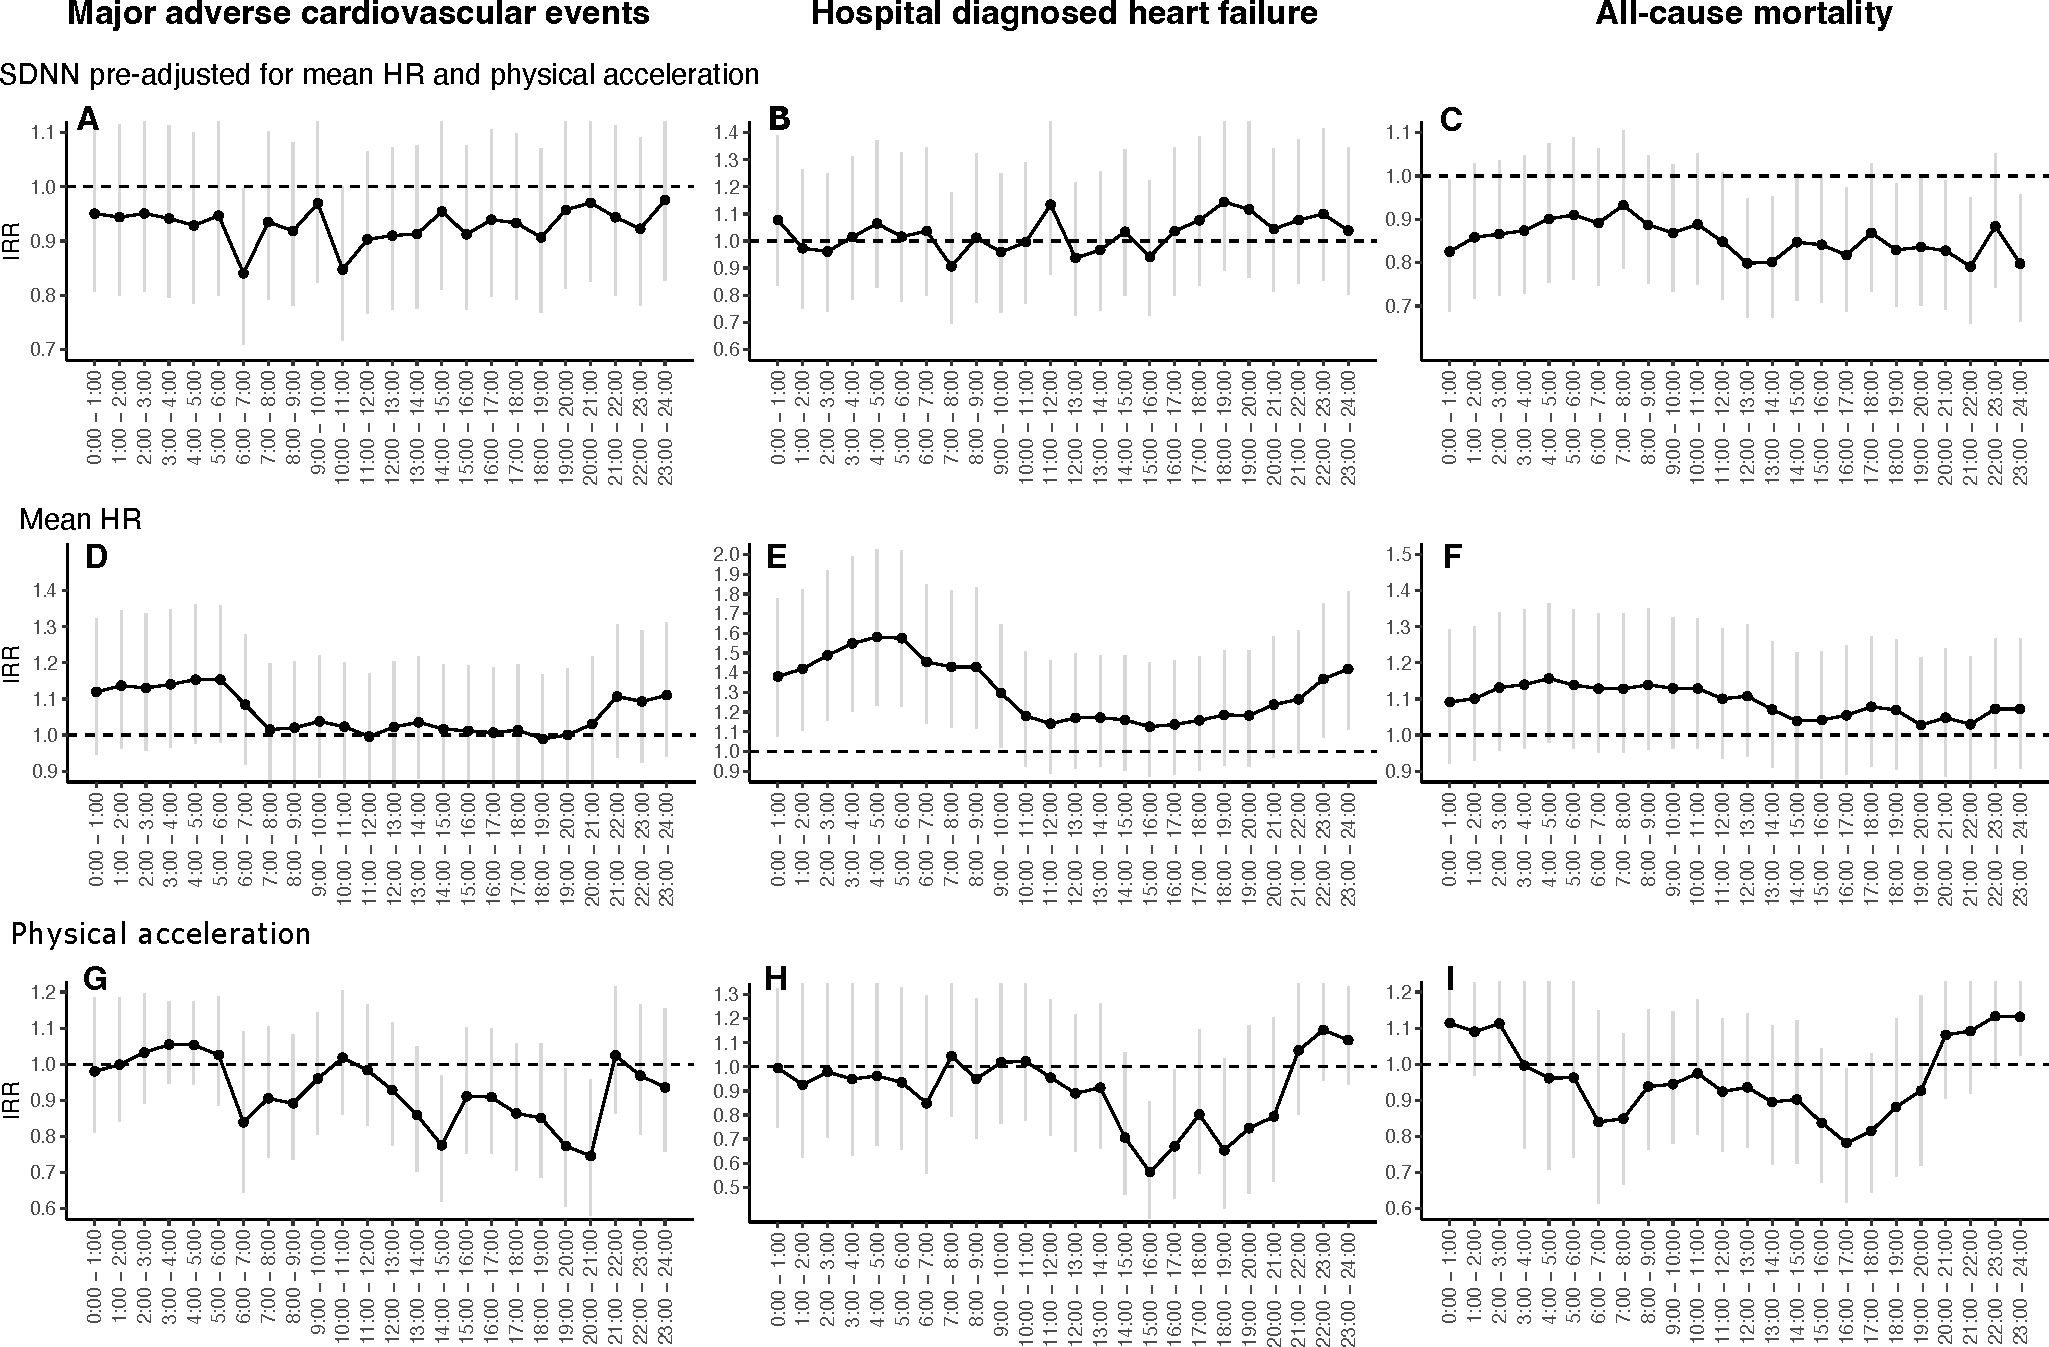
\includegraphics{images/figure_ADD_PRO_risk_by_hour.pdf}

\emph{SDNN preadjusted for concurrent physical acceleration and heart
rate, as well as mean heart rate (HR) and physical acceleration, were
measured hourly from 00:00 to 24:00. The IRR for MACE, heart failure
hospitalization, and all-cause mortality are shown by hourly
associations of: (A--C) preadjusted SDNN, (D--F) mean HR, and (G--I)
physical acceleration. Models were adjusted for age, sex, education,
alcohol consumption, smoking behavior, body mass index, total
cholesterol, and HbA1c. Figure adapted from Appendix Study
II\textsuperscript{87}}

}

\caption{\label{fig-ADD_PRO_risk_by_hour}\textbf{Diurnal heart rate
variability and heart rate association with major adverse cardiovascular
events, heart failure, and all-cause mortality risk}}

\end{figure}

\restoregeometry

\hypertarget{study-iii}{%
\section{Study III}\label{study-iii}}

\hypertarget{descriptive-2}{%
\subsection{Descriptive}\label{descriptive-2}}

In study III, 176 participants had measures of NT-proBNP. CAN was
present in 31\% (n = 54) of participants (36\% among those with valid
CAN measurements (Figure~\ref{fig-CAN} A)).\textsuperscript{88}
Meanwhile, 23\% (n = 40) were unable to complete the CART assessment
adequately, primarily due to insufficient air pressure during the
Valsalva manoeuvre (n = 21).\textsuperscript{88} Compare to those
without CAN, the participants with CAN were more women (41 \% vs 33 \%),
were more sedentary (45\% vs 36\%), had a higher proportion with prior
major CVD (41\% vs 23\%) and declined eGFR (\textless{} 60ml/min/1.73
m\(^2\)) (35\% vs 22\%), higher levels of triglyceride (median 2.05
mmol/L vs 1.95 mmol/ L), were slightly older (median 62 years vs 61
years), had longer duration of T2D (median 19 years vs 15 years), and
higher use SGLT2i (65\% vs 60\%) but lower use of GLP-1RA (63\% vs
70\%). No other difference in clinical characteristic was observed (see
Table~\ref{tbl-can}).\textsuperscript{88}

\newgeometry{top=2cm, bottom=2cm, inner=0.5cm, outer=0.5cm}

\hypertarget{tbl-can}{}
\begin{landscape}\begin{table}
\caption{\label{tbl-can}Study characteristics in The CANCAN Study (Study IIY) by CAN status }\tabularnewline

\centering\begingroup\fontsize{10}{12}\selectfont

\resizebox{\linewidth}{!}{
\begin{tabular}[t]{llllll}
\toprule
CAN status & Missing & Overall, N = 176 & CAN missing, N = 40 & No CAN, N = 82 & CAN, N = 54\\
\midrule
\cellcolor{gray!6}{Sex (Women)} & \cellcolor{gray!6}{0} & \cellcolor{gray!6}{68 (39\%)} & \cellcolor{gray!6}{19 (48\%)} & \cellcolor{gray!6}{27 (33\%)} & \cellcolor{gray!6}{22 (41\%)}\\
Age (years) & 0 & 63 (55; 70) & 68 (61; 75) & 61 (52; 69) & 62 (56; 68)\\
\cellcolor{gray!6}{BMI (kg/m²)} & \cellcolor{gray!6}{2} & \cellcolor{gray!6}{32 (28; 37)} & \cellcolor{gray!6}{30 (26; 34)} & \cellcolor{gray!6}{33 (28; 38)} & \cellcolor{gray!6}{33 (30; 36)}\\
Duration of diabetes (years) & 0 & 17 (11; 24) & 20 (13; 30) & 15 (9; 21) & 19 (13; 24)\\
\cellcolor{gray!6}{HbA1c (mmol/mol)} & \cellcolor{gray!6}{0} & \cellcolor{gray!6}{64 (56; 80)} & \cellcolor{gray!6}{65 (56; 85)} & \cellcolor{gray!6}{64 (55; 78)} & \cellcolor{gray!6}{64 (57; 76)}\\
\addlinespace
Total cholesterol (mmol/L) & 2 & 3.90 (3.23; 4.78) & 3.70 (3.33; 4.18) & 4.10 (3.33; 4.88) & 3.75 (3.03; 4.98)\\
\cellcolor{gray!6}{HDL (mmol/L)} & \cellcolor{gray!6}{2} & \cellcolor{gray!6}{1.00 (0.88; 1.20)} & \cellcolor{gray!6}{1.00 (0.90; 1.30)} & \cellcolor{gray!6}{1.00 (0.90; 1.20)} & \cellcolor{gray!6}{0.97 (0.80; 1.18)}\\
Triglycerides (mmol/L) & 3 & 2.00 (1.30; 2.90) & 2.10 (1.10; 2.80) & 1.95 (1.30; 2.90) & 2.05 (1.40; 2.98)\\
\cellcolor{gray!6}{Systolic blood pressure (mmHg)} & \cellcolor{gray!6}{1} & \cellcolor{gray!6}{133 (123; 143)} & \cellcolor{gray!6}{135 (127; 147)} & \cellcolor{gray!6}{131 (123; 142)} & \cellcolor{gray!6}{133 (120; 143)}\\
Diastolic blood pressure (mmHg) & 1 & 76 (68; 82) & 73 (66; 79) & 78 (72; 83) & 74 (66; 82)\\
\addlinespace
\cellcolor{gray!6}{Resting heart rate (bpm)} & \cellcolor{gray!6}{6} & \cellcolor{gray!6}{77 (66; 84)} & \cellcolor{gray!6}{68 (62; 80)} & \cellcolor{gray!6}{78 (69; 84)} & \cellcolor{gray!6}{80 (67; 89)}\\
Lying to standing (RR ratio) & 8 & 1.02 (1.01; 1.06) & 1.03 (1.02; 1.05) & 1.05 (1.01; 1.08) & 1.01 (1.00; 1.02)\\
\cellcolor{gray!6}{Deep breathing (RR ratio)} & \cellcolor{gray!6}{4} & \cellcolor{gray!6}{1.13 (1.07; 1.26)} & \cellcolor{gray!6}{1.15 (1.10; 1.28)} & \cellcolor{gray!6}{1.18 (1.11; 1.30)} & \cellcolor{gray!6}{1.07 (1.03; 1.08)}\\
Valsalva maneuver (RR ratio) & 45 & 1.24 (1.13; 1.36) & 1.20 (1.14; 1.25) & 1.32 (1.25; 1.45) & 1.11 (1.08; 1.16)\\
\cellcolor{gray!6}{NT-proBNP (pg/ml) categories} & \cellcolor{gray!6}{0} & \cellcolor{gray!6}{} & \cellcolor{gray!6}{} & \cellcolor{gray!6}{} & \cellcolor{gray!6}{}\\
\addlinespace
 < 50 &  & 72 (41\%) & 10 (25\%) & 47 (57\%) & 15 (28\%)\\
\cellcolor{gray!6}{ 50-124} & \cellcolor{gray!6}{} & \cellcolor{gray!6}{38 (22\%)} & \cellcolor{gray!6}{11 (28\%)} & \cellcolor{gray!6}{16 (20\%)} & \cellcolor{gray!6}{11 (20\%)}\\
125-300 &  & 28 (16\%) & 7 (18\%) & 10 (12\%) & 11 (20\%)\\
\cellcolor{gray!6}{> 300} & \cellcolor{gray!6}{} & \cellcolor{gray!6}{38 (22\%)} & \cellcolor{gray!6}{12 (30\%)} & \cellcolor{gray!6}{9 (11\%)} & \cellcolor{gray!6}{17 (31\%)}\\
Any antihypertensive medication (yes) & 0 & 140 (80\%) & 33 (83\%) & 61 (74\%) & 46 (85\%)\\
\addlinespace
\cellcolor{gray!6}{Beta-blockers (yes)} & \cellcolor{gray!6}{0} & \cellcolor{gray!6}{52 (30\%)} & \cellcolor{gray!6}{11 (28\%)} & \cellcolor{gray!6}{19 (23\%)} & \cellcolor{gray!6}{22 (41\%)}\\
Glucose-lowering medication &  &  &  &  & \\
\cellcolor{gray!6}{Metformin (yes)} & \cellcolor{gray!6}{0} & \cellcolor{gray!6}{123 (70\%)} & \cellcolor{gray!6}{26 (65\%)} & \cellcolor{gray!6}{56 (68\%)} & \cellcolor{gray!6}{41 (76\%)}\\
SGLT2-inhibitors (yes) & 0 & 81 (46\%) & 12 (30\%) & 40 (49\%) & 29 (54\%)\\
\cellcolor{gray!6}{GLP1 RAs (yes)} & \cellcolor{gray!6}{0} & \cellcolor{gray!6}{91 (52\%)} & \cellcolor{gray!6}{15 (38\%)} & \cellcolor{gray!6}{47 (57\%)} & \cellcolor{gray!6}{29 (54\%)}\\
\addlinespace
Insulin (yes) & 0 & 140 (80\%) & 33 (83\%) & 66 (80\%) & 41 (76\%)\\
\bottomrule
\multicolumn{6}{l}{\rule{0pt}{1em}\textit{Note: }}\\
\multicolumn{6}{l}{\rule{0pt}{1em}makecell[l]{Categorical variables: N (\%); Continous variables: Median (IQT:25th-75th\ Table are adapted from Table 1 in Appendix Study III}}\\
\end{tabular}}
\endgroup{}
\end{table}
\end{landscape}

\restoregeometry

\hypertarget{can-and-indicators-of-heart-failure}{%
\subsection{CAN and indicators of heart
failure}\label{can-and-indicators-of-heart-failure}}

A greater proportion of individuals with CAN were observed to exhibit
elevated NT-proBNP levels (\textgreater125 pg/ml) (51.9\%, n = 52/78)
compared to those without CAN (23.2\%, n = 26/112) (Figure~\ref{fig-CAN}
E).\textsuperscript{88} The fully adjusted odds ratio (OR) for elevated
NT-proBNP in individuals with CAN was 5.69 (95\% CI: 1.95; 18.49)
relative to those without CAN.\textsuperscript{88} Among the
cardiovascular autonomic reflex tests (CART), the Valsalva manoeuvre was
found to demonstrate the strongest association with NT-proBNP (OR 9.00,
95\% CI: 2.88; 33.09; n = 51/75), followed by deep breathing (OR 3.30,
95\% CI: 1.17; 9.77; n = 33/133) and orthostatic hypertension (OR 4.04,
95\% CI: 1.27; 13.77; n = 24/146).\textsuperscript{88} No significant
association was identified for the lying-to-standing test (OR 0.80, 95\%
CI: 0.32; 1.97; n = 54/108).\textsuperscript{88} After imputation of
missing CART data, the OR for CAN in relation to elevated NT-proBNP
declined to 2.94 (95\% CI: 1.37; 6.56).\textsuperscript{88} Sensitivity
analyses, which excluded participants using beta-blockers or those with
a history of CVD, resulted in a smaller sample size and wider confidence
intervals, though the overall association remained
unchanged.\textsuperscript{88} CAN was associated with elevated
NT-proBNP in individuals both without (NYHA I; OR = 4.3, 95\% CI: 1.1;
16.3) and with heart failure symptoms (NYHA ≥ II; OR = 16.4, 95\% CI:
1.2; 222.0), though the interaction was not statistically significant (p
= 0.4).\textsuperscript{88} Similar associations were observed across
WATCH-DM risk groups: very-low-to-moderate (OR = 6.1, 95\% CI: 1.6;
23.5) and high-to-very-high (OR = 6.3, 95\% CI: 0.83;
46.9).\textsuperscript{88} Participants with CAN were found to have 1.7
(95\% CI: 0.3 to 3.0) point higher WATCH-DM risk scores compared to
those without CAN.\textsuperscript{88} The OR of presenting with NYHA
class II or higher was 5.51 (95\% CI: 1.9 to 15.97) in the group with
CAN.\textsuperscript{88}

\newgeometry{top=2cm, bottom=2cm, inner=0.5cm, outer=0.5cm}

\begin{figure}

{\centering 

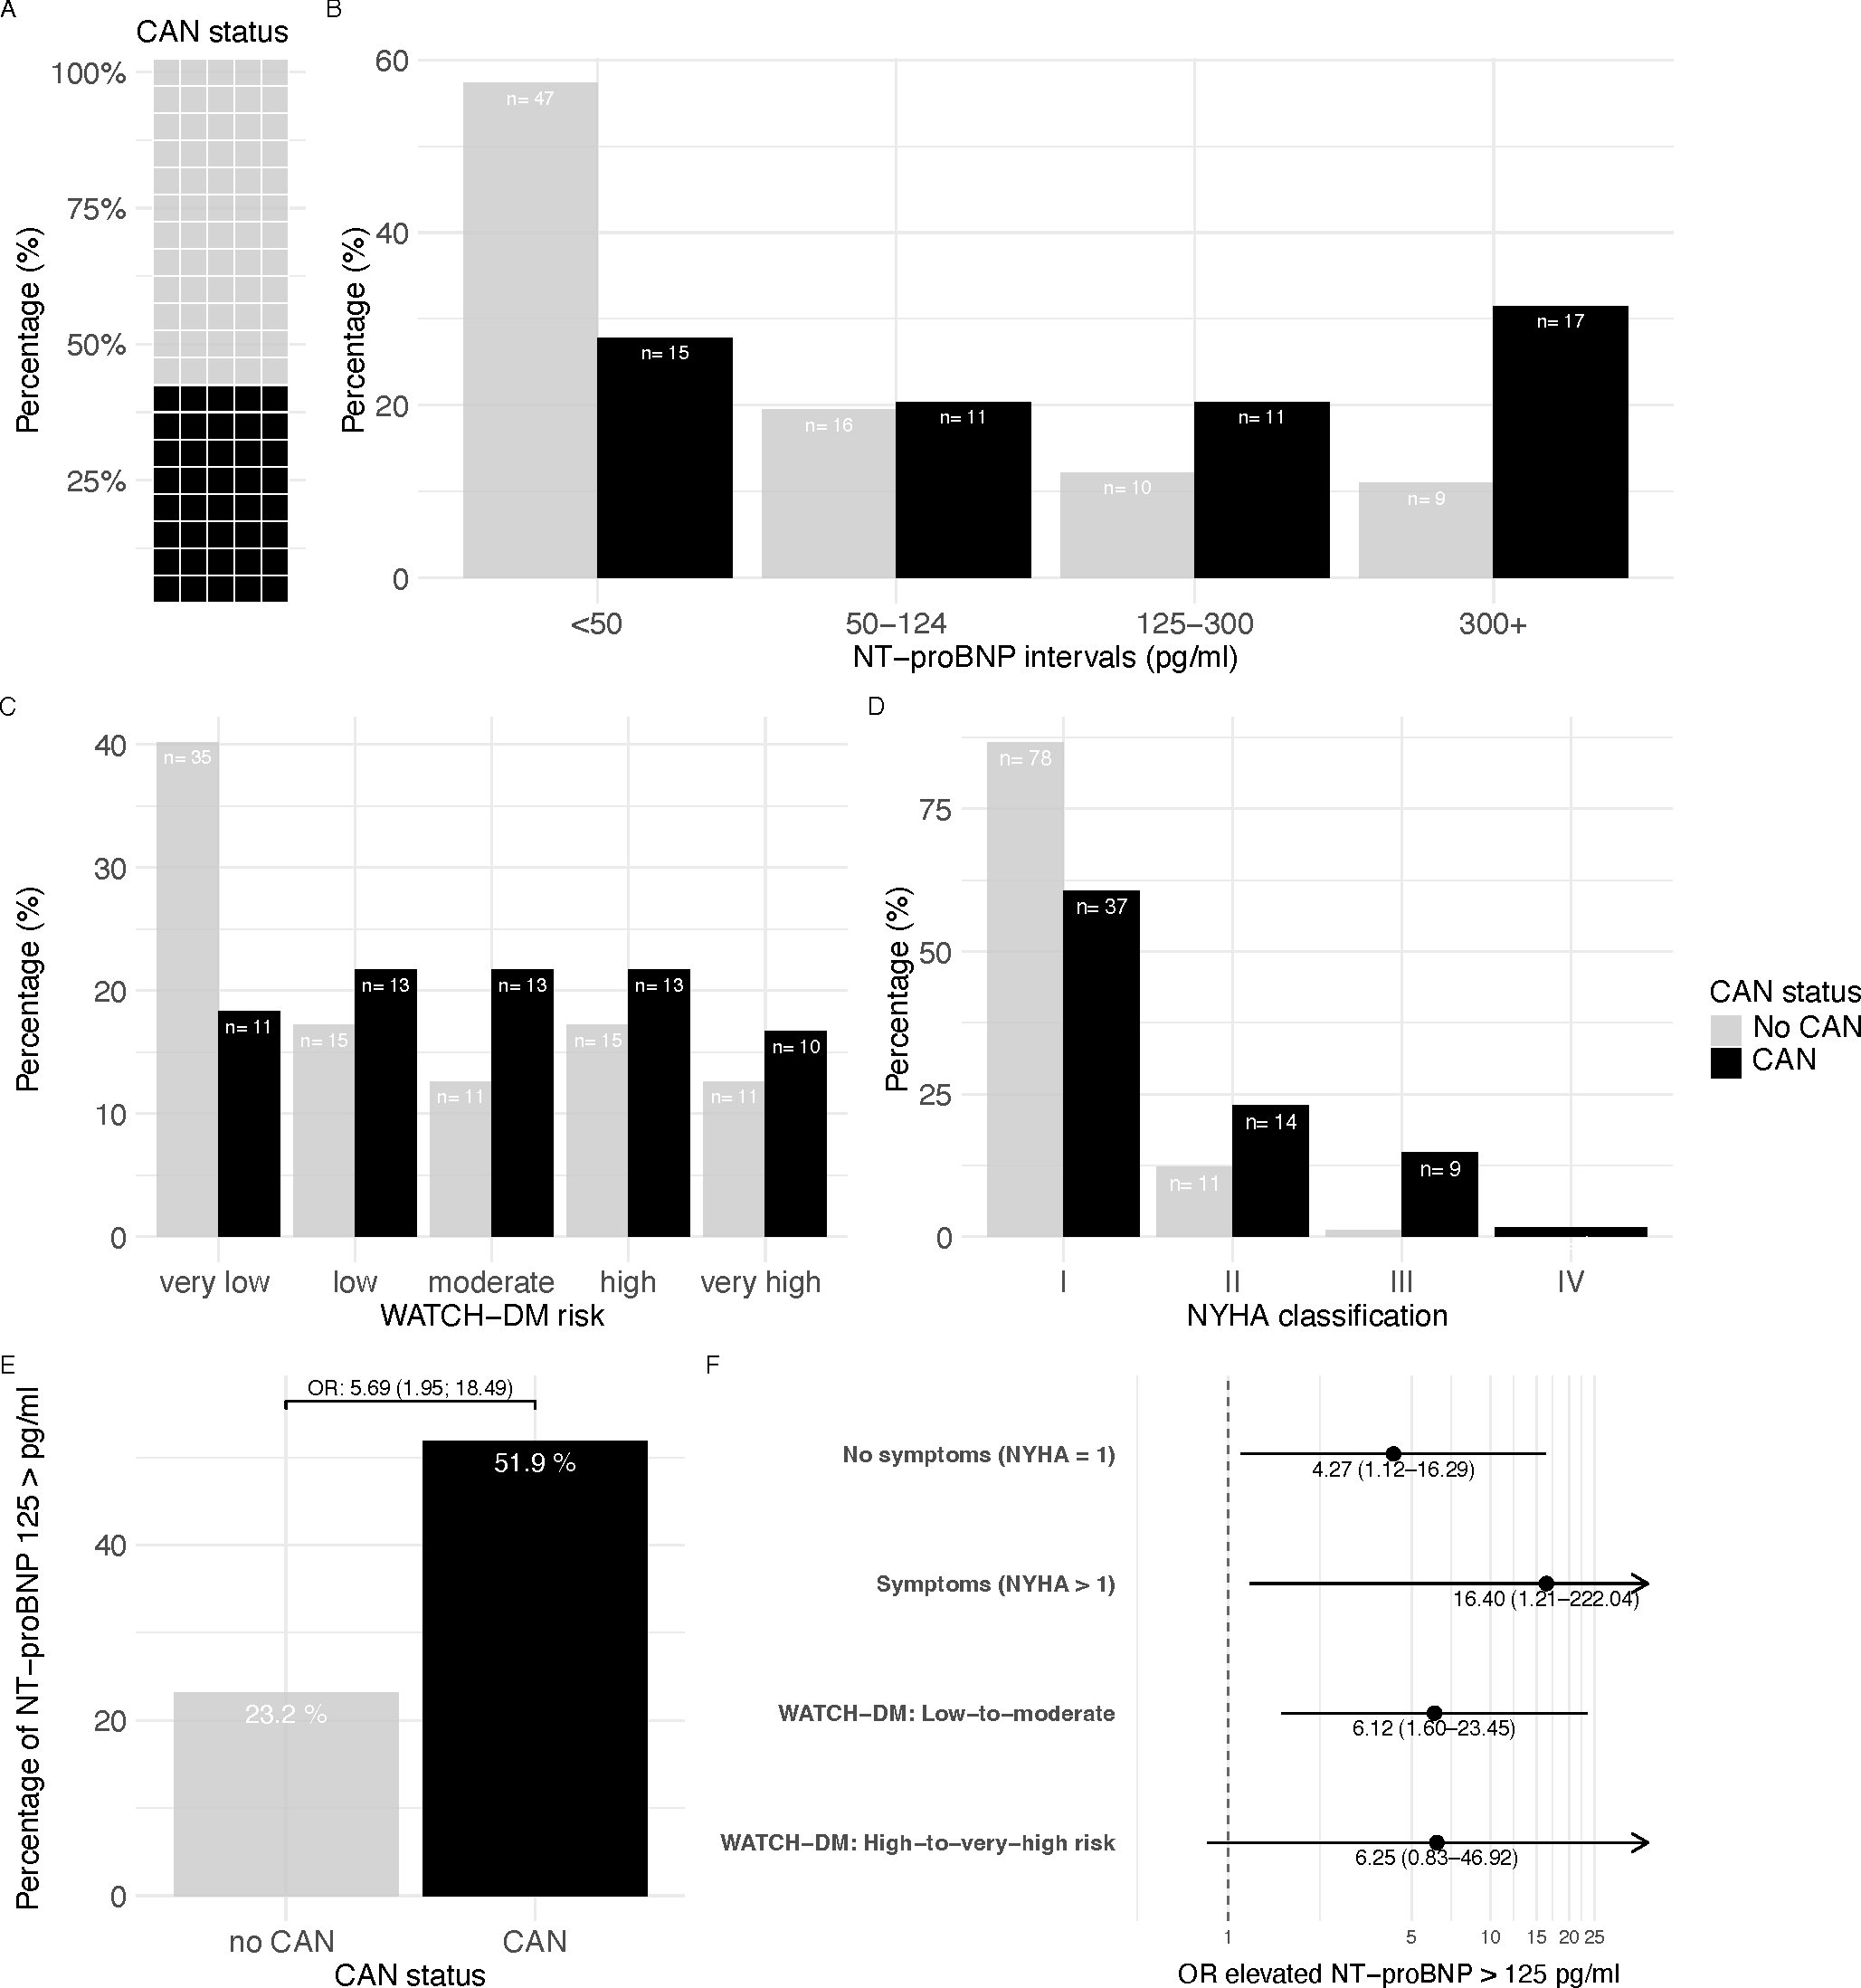
\includegraphics[width=0.85\textwidth,height=\textheight]{images/heart_failure_distribution_can_figure_2_2.pdf}

\emph{A: Percentage distribution by CAN status (no CAN, CAN). B:
Percentage distribution of NT-proBNP level categories stratified by
individuals with and without CAN. C: Percentage distribution of WATCH-DM
risk score stratified by individuals with and without CAN. C: Percentage
distribution of NYHA classification stratified by individuals with and
without CAN. E: Percentage of individuals with NT-proBNP \textgreater{}
125 pg/ml among those with and without CAN and adjusted odds ratio from
Model 4. F: Effect modification of the association between CAN and
NT-proBNP by symptoms defined by NYHA classification (symptoms: NYHA ≥
II vs no symptoms: NYHA = I) and risk score defined by WATCH-DM risk
(very-low-to-moderate vs high-to-very-high risk). Figure from Appendix
Study III\textsuperscript{88}}

}

\caption{\label{fig-CAN}\textbf{Distribution of NT-proBNP, NYHA Class,
and WATCH-DM Score by CAN Status, and association of CAN with Elevated
NT-proBNP}}

\end{figure}

\restoregeometry

\bookmarksetup{startatroot}

\hypertarget{discussion}{%
\chapter{Discussion}\label{discussion}}

\clearpage
\null
\thispagestyle{empty}
\clearpage

The aim of this dissertation is to understand how cardiovascular
autonomic dysfunction and CAN affect the risk of CVD across stages of
glucose metabolism. Given the rising prevalence of prediabetes and T2D,
and their association with increased risks of CVD and heart failure,
there is a pressing need for earlier indicators to help healthcare
providers intervene in a timely manner and prevent progression to more
advanced stages of cardiovascular complications. One promising approach
involves leveraging data from wearable devices and standardized
screening tools. Heart rate dynamics and variability across different
circumstances may hold promise as accessible indicators for timely
cardiovascular risk stratification.

This chapter presents a summary of the main findings from this
dissertation, interpreted in the context of existing evidence in the
field, and discusses their clinical relevance across different levels of
healthcare. Moreover, the strengths and limitations of the methods and
results will be discussed.

\newpage

\hypertarget{summary-of-findings}{%
\section{Summary of findings}\label{summary-of-findings}}

In this dissertation, autonomic dysfunction, defined by long-term HRV
and standardized CARTs, and its relationship with cardiovascular
complications were studied across three different cohorts representing
populations at varying levels of prevention and care, including public
health, primary care, and secondary care. In The Maastricht Study (Study
I), I investigated autonomic dysfunction, measured by 24-hour HRV, and
arterial stiffness, measured dynamically along the descending aorta and
locally at the carotid site among individuals with NGM, prediabetes, and
T2D. Lower HRV was associated with higher aortic and carotid stiffness.
This association was evident regardless of glucose metabolism status and
was more pronounced in individuals with prediabetes or T2D. The
modifying effect of dysglycemia was confirmed by a statistically
significant stronger association across higher HbA1c levels. Z-scores of
time- and frequency-domain measures showed the strongest associations,
primarily driven by HRV indices reflecting total variation in interbeat
intervals (SDNN, SDANN, SDNN index, ULF, VLF, TP).

Study II focused on individuals at higher risk of developing diabetes,
using data from the ADDITION-PRO cohort. In Study II, lower SDNN,
measured over multiple days, was associated with 18, 24, and 21 percent
higher risk per SD for ischemic-related CVD, hospitalization for heart
failure, and all-cause mortality, respectively. The risk became higher
at SDNN levels below 120 ms, supported by a greater difference in
incidence rates between individuals with 100 ms and 120 ms than the
difference observed between individuals with 120 ms and 160 ms. Hourly
measures suggested a specific time point related to ischemic-related
CVD, as lower SDNN recorded between 6:00 and 7:00 AM was associated with
MACE. Adjustment using the residuals method for concurrent heart rate
and physical movement did not explain the observed association. Hourly
SDNN was associated with all-cause MRR, although no specific time point
showed an exceptionally strong association. While no association between
hourly SDNN and heart failure was observed, higher heart rate during the
night hours from 02:00 to 06:00 AM was linked to a higher risk of heart
failure hospitalization.

These findings suggest that both long-term HRV measures and hourly HRV
responses may serve as indicators of CVD risk. However, a key
observation is that long-term HRV was assessed under free-living
conditions, which restricts the comparability of results to standardized
tests of autonomic function, although it provides insights that are more
comparable to what may be found with long-term wearable devices. In the
CANCAN Study (Study III), standardized CARTs were used to define CAN and
to describe indicators of heart failure, including elevated NT-proBNP,
WATCH-DM risk, and NYHA classification, among individuals with and
without CAN in a population with T2D. In CANCAN, two out of five had
CAN. Compared to individuals without CAN, these individuals more often
showed signs of heart failure, including elevated NT-proBNP levels,
higher WATCH-DM risk scores, and higher classifications on the NYHA. CAN
was associated with elevated NT-proBNP levels and these persisted even
among individuals without heart failure symptoms based on NYHA
classification, as well as among those categorized as having low to
moderate heart failure risk according to the WATCH-DM score.

In summary, various aspects of autonomic dysfunction and cardiovascular
complications were investigated in populations with NGM, prediabetes, or
T2D. The overall findings showed that autonomic function, assessed
through heart rate dynamics of long-term HRV and diurnal HRV or heart
rate responses to autonomic reflex tests, is associated with a higher
risk of CVD and heart failure. This relationship appears to be stronger
in more severe stages of dysglycemia. Moreover, among individuals with
T2D, the presence of CAN may help identify those at higher risk of heart
failure, even in the absence of heart failure symptoms.

\hypertarget{cardiovascular-autonomic-dysfunction-and-its-impact-on-heart-disease-across-glucose-metabolism}{%
\section{Cardiovascular autonomic dysfunction and its impact on heart
disease across glucose
metabolism}\label{cardiovascular-autonomic-dysfunction-and-its-impact-on-heart-disease-across-glucose-metabolism}}

This dissertation shows that autonomic dysfunction, measured by HRV and
CARTs, is associated with CVD risk across the spectrum of glucose
metabolism dysregulation. This association is evident in measures of
arteriosclerosis, atherosclerotic events, all-cause mortality, and heart
failure in individuals at high risk of diabetes, as well as in
indicators of heart failure in patients with T2D.

\hypertarget{arteriosclerosis-1}{%
\subsubsection{Arteriosclerosis}\label{arteriosclerosis-1}}

In Study I, autonomic dysfunction, measured by 24-hour HRV, was shown to
be cross-sectionally associated with arterial stiffness, measured both
dynamically (cf PWV) and locally (CD). Adjustments for demographic and
lifestyle factors, as well as a range of cardiovascular risk factors,
did not explain the association. This suggests that autonomic responses
under free-living conditions may contribute to the development of
arterial stiffness. The majority of studies in the field have shown an
association between autonomic dysfunction, as measured by short-term HRV
during rest, and arterial stiffness in populations with either type 1 or
T2D.\textsuperscript{98,99} Study I further extended this perspective by
examining long-term HRV in a population without diabetes or prediabetes.

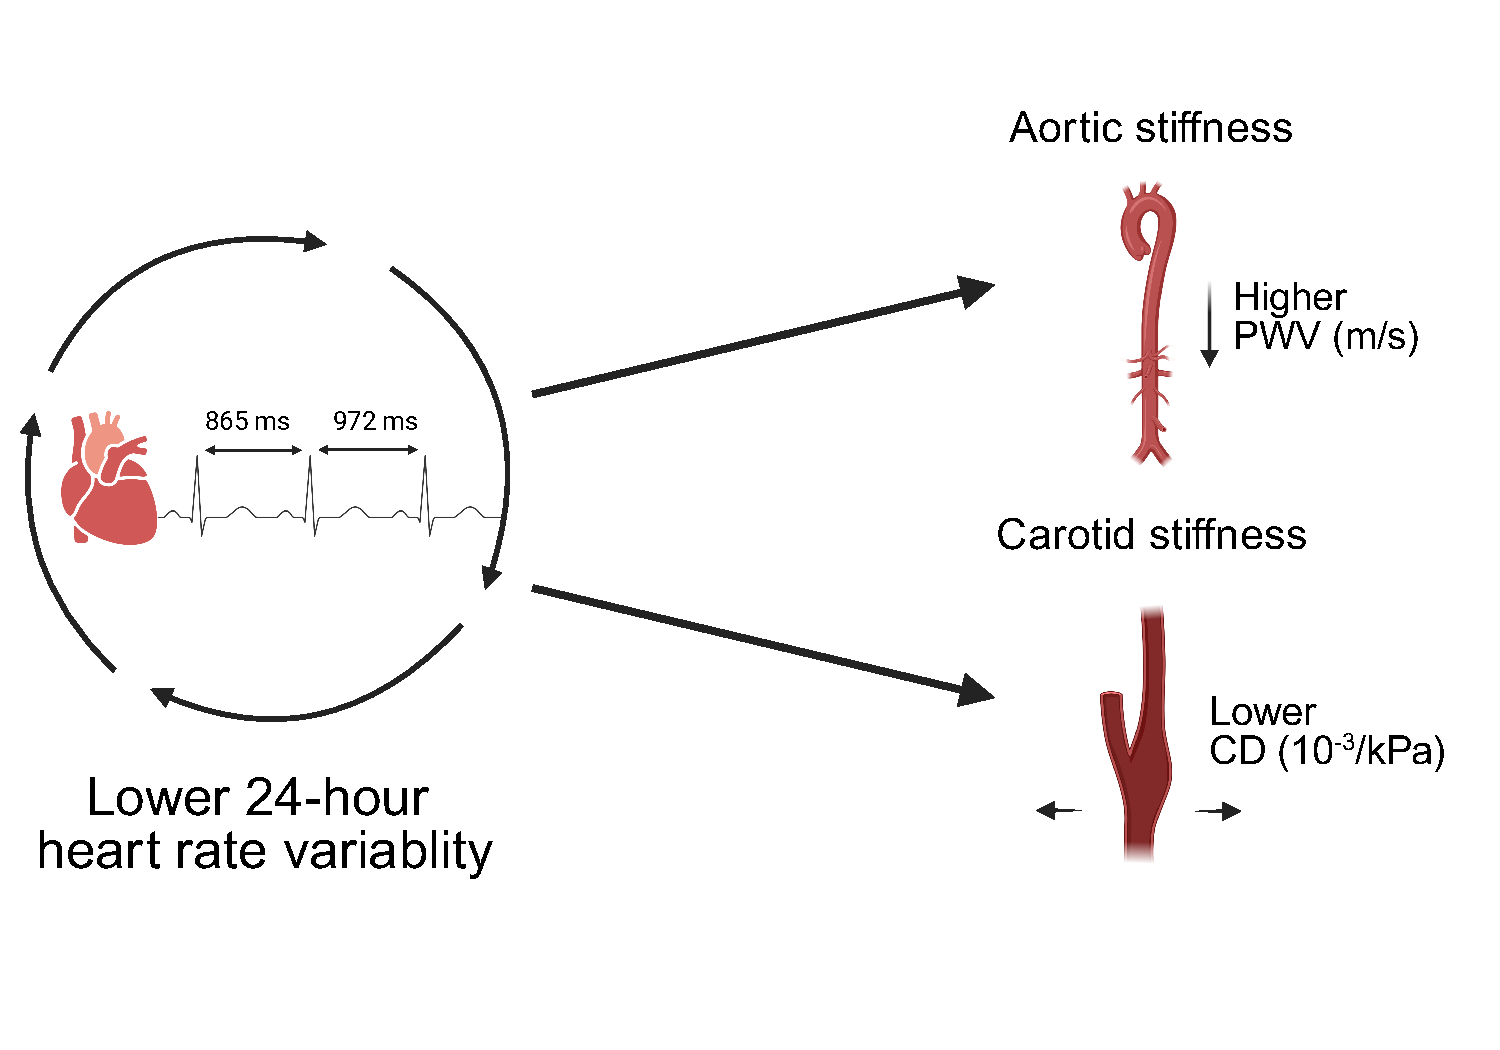
\includegraphics{images/hrv_arterial_stiffness.pdf} \emph{(Source:
Author)}

Arterial stiffness is not only a structural marker of vascular ageing
but is also dynamically modulated by local endothelial signals and
autonomic nervous system activity. Several studies have demonstrated a
link between elevated sympathetic tone and higher arterial
stiffness.\textsuperscript{100,101} Two possible mechanisms may explain
how autonomic dysfunction is related to arterial stiffness.

First, autonomic dysfunction may raise vascular tone in large arteries,
reducing elasticity. Animal studies support this, showing that proper
autonomic regulation is essential for maintaining aortic
elasticity.\textsuperscript{31} This effect may, in part, be transient
and reversible if autonomic function is restored. However, chronic
sympathetic overstimulation can lead to structural remodeling and
sustained stiffness.\textsuperscript{102} While such findings cannot be
directly extrapolated to humans, they suggest plausible biological
pathways.\textsuperscript{103}

Second, the autonomic nervous system controls heart rate and cardiac
contractility.\textsuperscript{101}{]} Autonomic dysfunction,
characterized by increased sympathetic activity and reduced
parasympathetic tone, elevates rHR and arterial shear stress,
potentially contributing to structural arterial stiffening. Data from
the Whitehall II study found that a steeper 10-year decline in
short-term resting HRV was associated with greater aortic stiffness five
years later.\textsuperscript{103}

The association between 24-hour HRV and arterial stiffness (Study II)
was modified by dysglycemia, suggesting dysglycemia may induce CAN that
can affect arterial stiffness, even before the onset of
T2D.\textsuperscript{8,104,105} Data from the Whitehall II study showed
that aortic stiffness increased more steeply with higher HbA1c values
among non-diabetic individuals\textsuperscript{106}, supporting this
notion. In the subpopulation in Study I without diabetes, a modification
by HbA1c in both aortic and carotid stiffness was observed. The
modifying effect of HbA1c suggests that hyperglycaemia amplifies the
consequences of autonomic dysfunction.

\hypertarget{atherosclerosic-events}{%
\subsubsection{Atherosclerosic events}\label{atherosclerosic-events}}

Study II showed that individuals with a preclinical stage of autonomic
dysfunction, measured by multiday HRV, face a higher risk of incident
ischemic CVD, heart failure, and all-cause mortality.

Multiday HRV was assessed to capture autonomic activity in real-life
settings across several days. These results are consistent with earlier
research linking lower HRV (including measures from 10 seconds to 24
hours) to CVD and mortality.\textsuperscript{5,107} Findings from Study
II build on existing evidence by: (1) focusing on a population at
elevated risk for diabetes, (2) employing multiday HRV recordings, and
(3) identifying specific times of day when HRV patterns were indicative
of ischemic-related cardiovascular risk. By using both week-long and
hourly data, specific periods that better indicate long-term risk were
identified. A strength of using multiday HRV recordings is that they
provide more robust insights into individual autonomic patterns by
averaging autonomic responses across typical daily conditions. This
reduces the influence of random fluctuations caused by factors such as
physical activity, emotional states, or sleep on any single
day.\textsuperscript{108}

Multiple mechanisms may explain how autonomic dysfunction contributes to
the initiation and progression of ischemic events and stroke. First, as
discussed in Study I, autonomic dysfunction may contribute to arterial
stiffness, a dynamic and potentially modifiable process that impairs
vasodilation and increases hemodynamic stress\textsuperscript{109--111},
thereby elevating the risk of ischemic events.

Second, the autonomic nervous system innervates the adventitia layer of
blood vessels, modulating vascular tone via sympathetic
fibres.\textsuperscript{32}Although plaques form in the intima, higher
plaque burden has been linked to increased local sympathetic nerve
density, possibly through neuroinflammatory
pathways.\textsuperscript{112} Autonomic dysfunction likely exerts
systemic effects on the vasculature\textsuperscript{32}, making a direct
role in plaque formation uncertain, but it may compromise vasodilatory
capacity during ischemic or thrombotic events. Notably, reduced
sympathetic innervation has attenuated plaque formation in animal
models, supporting indirect effects on
atherogenesis.\textsuperscript{112}

Third, autonomic dysfunction has been shown to interfere with signalling
pathways controlling heart rhythm, potentially leading to arrhythmias.
Earlier studies have shown lower short-term HRV was associated with
incident atrial fibrillation (AF), with a higher risk among participants
with T2D.\textsuperscript{107,113} This supports the role of autonomic
dysfunction in arrhythmogenesis, which increases the risk of myocardial
infarction and stroke.\textsuperscript{114} Study II did not include
atrial fibrillation (AF) as an outcome due to limitations in Danish
registries prior to 2016, which often failed to distinguish between
short- and long-term AF, thereby compromising diagnostic
validity.\textsuperscript{115}

Study II focused on long-term HRV under free-living conditions,
capturing stress-responsive periods such as morning awakening. These
recordings likely reflect underlying autonomic dynamics relevant to
cardiovascular risk. A Genome-Wide Association Study (GWAS) in the UK
Biobank of short-term HRV supports this by identifying mechanisms
involving G-protein signaling, pacemaker activity, and mitochondrial
function as likely mediators of the genetic contribution to HRV. These
pathways influence vagal control, cardiac excitability, and energy
metabolism.\textsuperscript{116} Although derived from short-term
recordings, these genetic associations may reflect autonomic traits that
persist across different time scales and reinforce the notion of a
biological basis for inter-individual differences in HRV, preceding and
independent of the onset of dysglycaemia. A Mendelian randomization
study using data from the Rotterdam Study found that genetically
predicted HRV was associated with a higher risk of
AF.\textsuperscript{117} However, this association did not extend to
all-cause mortality or cardiovascular death in the UK Biobank cohort,
where only phenotypically measured HRV showed a significant relationship
with these outcomes.\textsuperscript{118} Interestingly, the genetic
determinants of HRV exhibited pleiotropic relationships with several
autonomic traits, including resting heart rate, heart rate response
during exercise, and post-exercise recovery
dynamics.\textsuperscript{118} No GWAS has yet been conducted for
long-term HRV. Therefore, it is unclear whether the genetic influences
identified for short-term HRV are applicable to long-term HRV. Future
GWAS efforts targeting long-term HRV could help establish causal
relationships to CVD by leveraging methods such as Mendelian
randomization and advancing understanding of the genetic architecture
underlying autonomic regulation under a full day.

\hypertarget{heart-failure-1}{%
\subsubsection{Heart failure}\label{heart-failure-1}}

The relationship between cardiovascular autonomic dysfunction and heart
failure is complex.\textsuperscript{119} On one hand, autonomic
dysfunction contributes to cardiac remodelling and eventual heart
failure.\textsuperscript{30,120} On the other hand, it may reflect
compensatory mechanisms of the progression of cardiac remodelling and
declining cardiac output.\textsuperscript{30} Findings in Study I and II
demonstrated a relationship between autonomic dysfunction and heart
failure both cross-sectionally in a population with T2D and
prospectively in individuals representing different tiers of diabetes
risk. However, the extent to which this relationship supports one
explanation over the other is difficult to determine due to limitations
in the data, as both baseline and follow-up measures of heart failure
and HRV are lacking.

Previous studies have shown that both short- and long-term HRV are
associated with incident heart failure in populations with and without
T2D.\textsuperscript{121--124} Findings from Study \,II extended prior
work by applying multiday HRV recordings to a population at high risk
for diabetes and by: (1) assessing the role of resting heart rate in the
HRV--heart failure relationship, and (2) identifying time-of-day heart
rate patterns associated with heart failure risk.

Several mechanisms may underlie this relationship. Arterial stiffness is
known to contribute to cardiac remodelling by increasing cardiac
afterload and reducing coronary perfusion through earlier return of the
reflected pulse wave.\textsuperscript{125} This suggests that autonomic
dysfunction may indirectly influence heart failure through arterial
stiffness. However, structured methods such as mediation analysis with
repeated measures are needed to clarify these pathways.

Study II showed that multiday HRV was associated with incident heart
failure, and approximately one-fourth of the risk was explained by
resting heart rate. Data from the Rotterdam Study showed that resting
short-term HRV was longitudinally associated with echocardiographic
measures reflecting systolic function, suggesting that autonomic
dysfunction contributes to cardiac remodelling.\textsuperscript{120} In
contrast to MACE outcomes, findings from Study II showed no specific
time point in hourly HRV that was associated with heart failure.
Instead, it was the overall daily pattern captured by multiday HRV that
was linked to heart failure risk. This suggests that the association is
not driven by isolated shifts in autonomic activity in response to
circadian stressors, but rather by a consistently impaired autonomic
balance under free-living conditions.

In Study III, individuals with CAN were found to have higher risk of
elevated NT-proBNP, a biomarker of myocardial stress and early heart
failure. This supports the interpretation that CAN contributes to both
structural and functional cardiac changes, reflected in elevated
NT-proBNP levels.

Reverse causation cannot be ruled out, as autonomic dysfunction may also
reflect compensatory responses to progressing heart
failure.\textsuperscript{30} CAN and cardiac remodelling may interact in
a reinforcing cycle: autonomic dysfunction increases sympathetic tone
and reduces parasympathetic modulation, promoting cardiac stress and
remodelling, which in turn further impairs autonomic
regulation.\textsuperscript{24} This feedback loop may accelerate heart
failure progression, although this remains beyond the scope of the
current data and analysis.

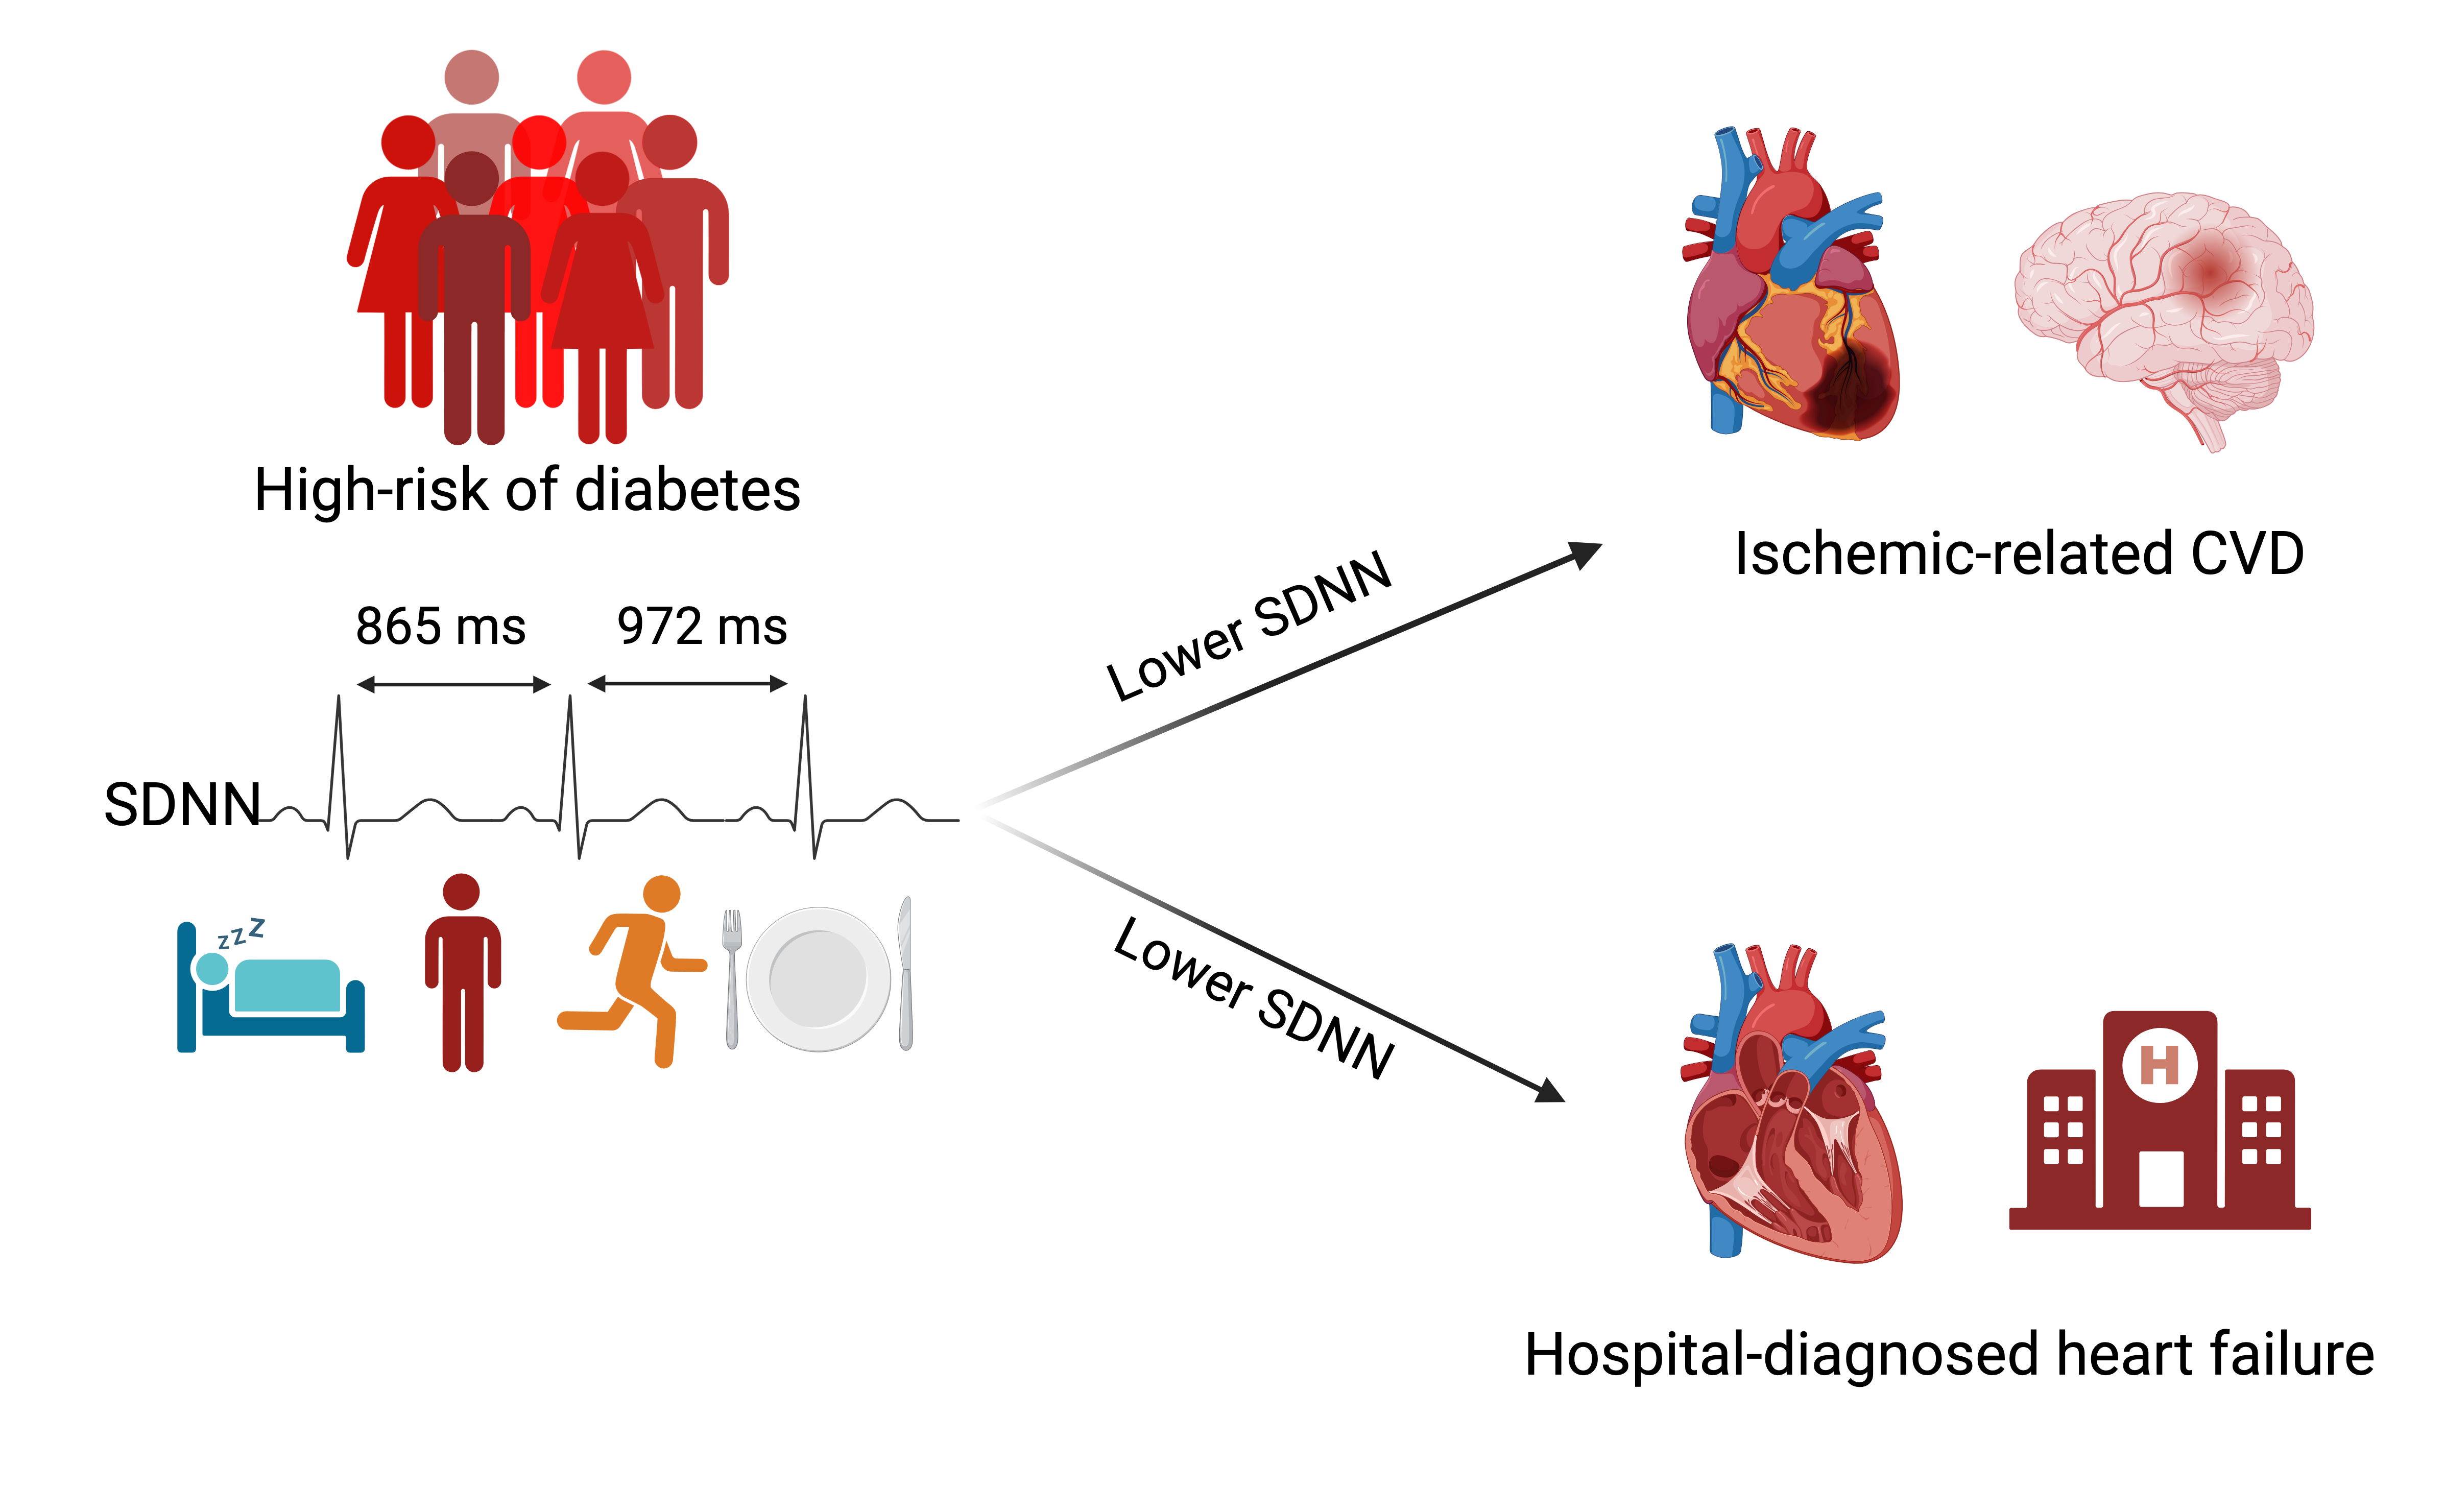
\includegraphics{images/ADD_PRO_IMG.png} \emph{(Source: Author)}

\hypertarget{clinical-implications}{%
\section{Clinical implications}\label{clinical-implications}}

The dissertation investigates autonomic dysfunction in populations
ranging from NGM to T2D and yields insights relevant for individuals who
engage with the healthcare system at different levels. No specific role
has yet been defined for autonomic dysfunction in clinical
decision-making within healthcare, as current treatment and intervention
options specifically targeting autonomic function remain limited.
Although the results do not point directly to where and how
implementation of autonomic dysfunction in clinical practice may make
sense, the included studies broadly represent situations relevant to
public health, primary care, and secondary care settings. In the
following section, the clinical implications of using autonomic
dysfunction in the prevention of CVD will be discussed. If long-term HRV
or CARTs are to be considered for improving risk stratification, it is
important to determine at what stage in the progression of diabetes
risk, and at which level of care, autonomic dysfunction becomes
meaningful for early detection and intervention.

\hypertarget{public-health}{%
\subsection{Public health}\label{public-health}}

A central strategy in preventing CVD is the early identification and
multifactorial treatment of individuals at high
risk.\textsuperscript{126} Public health initiatives support this by
promoting healthy lifestyles, facilitating early screening for risk
factors, and improving access to essential care and
medications.\textsuperscript{127,128} Long-term HRV may enhance these
efforts by identifying individuals with elevated cardiovascular risk and
by tracking their physiological response to lifestyle changes.

Evidence from Study I showed that lower long-term HRV was associated
with higher arterial stiffness, as measured by cf-PWV and CD, even in
individuals without T2D. One standard deviation lower HRV corresponded
to the effect of 2.7 additional years of ageing on aortic stiffness
(cf-PWV) and 1.6 years on carotid stiffness (CD).\textsuperscript{77}
These cross-sectional findings suggest that HRV may serve as a marker of
early vascular ageing and cardiovascular risk. Supporting this, the
Whitehall II study demonstrated a longitudinal relationship between
short-term HRV and aortic stiffness.\textsuperscript{103} Together,
these findings highlight the potential of HRV as an indicator of
vascular health.

Within the public health setting, individuals with prediabetes represent
a particularly vulnerable group at risk for
comorbidities.\textsuperscript{129} They often fall between structured
care pathways, sometimes encouraged to reassess their cardiovascular
risk at more frequent intervals, other times not offered any additional
measures or attention beyond general lifestyle advice. Notably, Studies
I and II demonstrated that the associations between long-term HRV and
CVD risk were especially pronounced in this population. In those at high
risk of diabetes, a one standard deviation (33 ms) lower multiday SDNN
was equivalent to 4.5 additional years of ageing for ischemic-related
CVD and 2.2 to 2.4 years for heart failure.\textsuperscript{87} On a
population level, lower HRV (SDNN: 100 ms) in individuals with
prediabetes was associated with a higher incidence rate of CVD, heart
failure, and all-cause mortality compared to individuals with
normal-to-higher HRV (SDNN: 120 to 160 ms). These findings reinforce the
role of HRV as an early and sensitive marker of cardiovascular health in
populations at cardiometabolic risk.

While these findings highlight HRV's potential, practical implementation
faces several challenges. Historically, long-term HRV monitoring has
required specialized equipment such as Holter ECG
recorders.\textsuperscript{6} However, the growing popularity of
wearable devices offers a promising alternative.\textsuperscript{130}
These devices provide a non-invasive, user-friendly way to collect heart
rate and HRV data over time, under free-living conditions like those
examined in Study II.\textsuperscript{11}

If HRV monitoring proves effective in helping individuals maintain a
healthy, age-adjusted HRV range through lifestyle changes and prompts
healthcare engagement when HRV deteriorates, it could become a
meaningful tool for long-term health tracking. A cross-sectional study
of 8 million individuals found that those who took more steps per day
had higher HRV, suggesting that HRV may also reflect a healthy
lifestyle.\textsuperscript{13} This notion has been longitudinally
supported in the Whitehall II study.\textsuperscript{131} In addition to
the ADDITION-PRO study, the inclusion of data from future observational
cohorts that incorporate wearable devices, along with precise lifestyle
measures such as physical activity, diet, and sleep, could enhance the
understanding of patterns influencing long-term heart rate variability
and diurnal autonomic responses.\textsuperscript{132,133}

A major public health challenge lies in ensuring equitable access to
wearable technology.\textsuperscript{11}Individuals from lower
socioeconomic backgrounds are less likely to own such devices, raising
concerns about health disparities.\textsuperscript{11} Despite this,
there is encouraging evidence that the general population is open to
share health data with public institutions and support the use of AI in
disease monitoring.\textsuperscript{11,134}

In summary, integrating wearable HRV monitoring into public health
strategies could represent a transformative step in proactive
cardiovascular care. It holds potential for early detection,
personalized prevention, and timely referral to primary care when risk
levels increase.

\hypertarget{primary-care}{%
\subsection{Primary care}\label{primary-care}}

Cardiovascular risk in primary care is assessed using clinical
evaluations and standardized risk prediction tools to identify
individuals at elevated risk.\textsuperscript{135} Management focuses on
lifestyle modification, pharmacological therapy, and regular monitoring
to reduce cardiovascular events.\textsuperscript{135} In this health
care setting, long-term HRV may offer added value by improving the
precision of cardiovascular risk stratification and by serving as a
marker to monitor the effectiveness of preventive strategies.

Long-term HRV may improve ranking of individual risk when added to
established clinical risk scores. Tools such as SCORE2 and the
Framingham Risk Score are widely used in primary care to guide
cardiovascular risk assessment.\textsuperscript{136,137} In Study I,
models adjusted for conventional CVD risk factors supported the
potential added value of 24-hour HRV in relation to arterial stiffness,
a surrogate marker of CVD risk. Study II extended this perspective by
demonstrating associations between multiday HRV and incident CVD and
heart failure. However, these findings are based on associations and do
not include formal prediction modeling\textsuperscript{138}, and
therefore cannot determine whether incorporating long-term HRV or CARTs
into existing risk scores improves predictive performance beyond current
guidelines. This study design was not feasible in ADDITION-PRO, as the
cohort did not represent high-risk diabetes populations typically
identified in primary care (e.g., elevated HbA1c). Likewise, CANCAN is
limited by its small sample size and recruitment from secondary care. To
assess predictive value, cohorts should reflect individuals with T2D or
those at high risk, as defined by current clinical practice. Few studies
suggest that 24-hour HRV may improve risk discrimination for CVD and
all-cause mortality in individuals with T2D\textsuperscript{139}, and
for stroke and heart failure in older adults.\textsuperscript{121,140}
However, these studies often lack calibration or validation in
large-scale cohorts and have not been integrated with widely used risk
scores such as SCORE2 or the Framingham Risk Score.

Long-term HRV may also help classify preclinical autonomic dysfunction,
enabling targeted interventions in a subgroup of patients to prevent
CVD. The increasing availability of wearable devices capable of
capturing long-term HRV data presents a practical opportunity for
continuous monitoring in primary care. These devices may facilitate
earlier detection of autonomic dysfunction and support more personalized
approaches to cardiovascular risk management. However, the clinical
utility of stratifying patients based on preclinical autonomic
dysfunction remains uncertain. These considerations are only actionable
if interventions in this subgroup can be shown to lower cardiovascular
risk. Emerging evidence suggests that both pharmacological and lifestyle
interventions can improve HRV in the short
term.\textsuperscript{141--143} For example, high-intensity interval
training has been shown to improve autonomic function in obese
individuals with and without T2D.\textsuperscript{144} Similarly,
lifestyle changes in individuals with prediabetes have been associated
with improvements in short-term HRV, which may partly explain a
reduction in diabetes risk independently of weight
loss.\textsuperscript{145} Nevertheless, it remains unclear whether
these effects on HRV are sustainable over time and whether they
translate into long-term cardiovascular protection. In many cases,
improvements in autonomic function may be mediated indirectly through
changes in cardiometabolic markers such as glucose levels, lipid
profiles, body weight, maximal oxygen uptake, and blood
pressure.\textsuperscript{145--147}

Despite these uncertainties, monitoring autonomic function through
long-term HRV may offer a valuable tool for assessing cardiovascular
risk and tracking the impact of preventive strategies. In Denmark,
prediabetes, defined by HbA1c, is present in 7.1\% of
adults.\textsuperscript{148} One in five of these individuals develops
T2D within five years\textsuperscript{148}, while others either remain
in the prediabetic stage or return to normoglycemia. Despite their
higher risk of CVD and heart failure\textsuperscript{149}, individuals
with prediabetes are not captured by existing preventive strategies.
This underscores the need for early and precise risk
assessment.\textsuperscript{10} Given that the cardiovascular
consequences of autonomic dysfunction appear to be more pronounced in
individuals with prediabetes compared to those with normoglycemia, HRV
has the potential to help identify those at elevated CVD risk within
this group. However, evidence demonstrating improved risk prediction and
sustained effects leading to better cardiovascular outcomes is needed to
establish its relevance for integration into primary care.

\hypertarget{secondary-care}{%
\subsection{Secondary care}\label{secondary-care}}

In secondary care, endocrinologists assess cardiovascular and heart
failure risk by integrating advanced diagnostics, biomarker analysis,
and imaging to detect early heart failure, guided by symptoms and risk
profiles. The treatment of patients with T2D is guided by evidence-based
therapies and multidisciplinary collaboration.\textsuperscript{4,58,72}
The ADA/EASD 2022 consensus on Management of Hyperglycemia in T2D
emphasizes that early detection of heart failure in individuals with T2D
is crucial. This enables timely initiation of therapies such as SGLT2i,
which have demonstrated significant benefits in lowering heart
failure-related outcomes.\textsuperscript{72} A major challenge in
diabetes care is detecting heart failure before symptoms appear, as
patients with symptomatic heart failure face a higher risk of mortality
and more frequent hospitalizations.\textsuperscript{4} The AHA, ACC, and
HFSA 2022 guidelines recommend identifying individuals at risk of heart
failure based on factors such as diabetes, poor glycaemic control,
uncontrolled hypertension, hyperlipidaemia, elevated BMI, albuminuria,
renal dysfunction, and a history of CVD.\textsuperscript{58} Still,
there is a need to identify optimal approaches for recognizing and
diagnosing heart failure in clinical care, as broad echocardiographic
screening in T2D is time-consuming and costly.\textsuperscript{4}

Study III demonstrated that CAN may help identify individuals at higher
risk of heart failure, beyond what is captured by symptoms or existing
risk scores. These findings support considering CAN as a relevant risk
factor for heart failure and suggest it may have value in future risk
stratification strategies in T2D. A clinical advantage of using CARTs is
that they are standardized tests performed under controlled
conditions.\textsuperscript{70,89} CARTs have proven to be reliable and
reproducible, with reference values established in large population
studies.\textsuperscript{70,89} Beyond these findings and the
established evidence of higher heart failure risk, CAN also identifies
individuals at high risk for overall CVD, kidney disease, and early
mortality in the T2D population.\textsuperscript{63,64} In Study III, I
observed that two out of five participants had CAN, highlighting it as a
complication with considerable prevalence. Theore, detecting CAN may
uncover an often-overlooked condition that is common in individuals with
T2D.

Clinical stratification of care includes two key considerations: (1) CAN
should be further evaluated for associated cardiovascular complications,
such as heart failure; and (2) cardiopreventive strategies should be
initiated earlier in this subgroup.

First, patients with CAN may benefit from further cardiovascular
assessment, including the use of sensitive biomarkers or
echocardiography. NT-proBNP is a strong predictor of heart failure and a
validated biomarker for ruling out the condition.\textsuperscript{58}
However, its specificity varies across heart failure phenotypes, being
less specific for detecting HFpEF compared to HFrEF.\textsuperscript{58}
Therefore, additional evaluation using echocardiography are warranted.
Beyond classifying heart failure phenotypes, echocardiography identifies
preclinical stages of heart failure through the detection of functional
or structural cardiac abnormalities. Including CAN in structured
assessments of heart failure could help clarify to which extent CAN
overlaps with cardiac abnormalities. Determining the diagnostic and
prognostic value of CAN, particularly its sensitivity and specificity in
detecting HFrEF and HFpEF, requires further investigation.

Second, the presence of CAN may justify earlier initiation of protective
therapies. SGLT2i are recommended as second-line treatment in T2D and
have demonstrated benefits in lowering the risk of heart failure, CVD,
and kidney function decline, complications commonly associated with
CAN.\textsuperscript{63,64} Current guidelines recommend initiating
these therapies based on a history of CVD, heart failure, or the
presence of conventional high-risk cardiovascular
factors.\textsuperscript{72} However, the specific impact of SGLT2i on
the progression of cardiorenal outcomes in patients with CAN remains to
be fully understood. Furthermore, while antihypertensive treatment is a
cornerstone of cardiovascular risk management, whether specific classes
of antihypertensive agents offer protective effects in patients with CAN
remains to be explored.

The direct clinical implications of the findings in Study III are
limited. The generalizability of the results is restricted, as the study
population consisted of patients with T2D receiving secondary care. Two
out of five patients with CAN showed to have a history of CVD, a group
already at higher risk of heart failure due to their prior diagnosis.
This overlap may influence the interpretation of CAN as an independent
risk factor. Therefore, these findings need to be validated in a broader
population with T2D, including individuals without a history of CVD.
Doing so would allow for greater generalizability of the results to the
broader T2D population, particularly those receiving care in primary
settings.

\hypertarget{strengths-and-limitations}{%
\section{Strengths and limitations}\label{strengths-and-limitations}}

\hypertarget{study-design}{%
\subsection{Study design}\label{study-design}}

\emph{Cross-sectional design}

Studies I and III are based on cross-sectional data, with exposure and
outcome measured within a three-month period. The main limitation of
this design is that it does not allow us to determine whether the
exposure led to the outcome or vice versa. As a result, temporality
cannot be established, nor can it be confirmed whether changes in the
outcome were caused by the exposure. Based on prior evidence, the
direction of the associations in Study I was inferred using
physiological knowledge and findings from epidemiological and in vivo
studies.\textsuperscript{103}

Study III focused on the clinical diagnosis of CAN and the presence of
heart failure. The research question was oriented toward the clinical
utility of CAN in identifying patients with T2D who may be progressing
early toward heart failure. Whether cardiac function progressively
worsens due to the underlying mechanisms of CAN remains to be fully
established.\textsuperscript{88}

\emph{Longitudinal design}

A major strength of Study II is its longitudinal design, where HRV was
measured at baseline and outcomes were captured prospectively through
national registries. This temporal structure ensures that the exposure
(HRV) preceded the outcome, lowering the risk of reverse causation. The
prospective design allows for stronger inference of directionality than
cross-sectional studies. Furthermore, the use of high-quality registry
data ensures complete outcome ascertainment and minimizes loss to
follow-up bias.

Causality cannot be ascertained from the findings in Study I and Study
II, and more causally focused methods are needed. These will be
discussed in detail in the \emph{Perspectives} section.

\hypertarget{internal-validity}{%
\subsection{Internal validity}\label{internal-validity}}

Cardiovascular autonomic function was assessed in this project both
under free-living conditions and in response to standardized test
procedures conducted during clinical visits. Additionally, dynamic
measurements were used to evaluate arterial stiffness both locally and
by velocity, and biomarker assessments were performed to determine the
presence of heart failure. In this section, the validity of 24-hour,
multiday, and hourly HRV measurements is discussed, along with the
standardized tests of CAN. The validity of the included outcomes is also
addressed, and the strengths and limitations of using MACE as a
time-to-event outcome are examined.

\hypertarget{long-term-hrv-24-hours-and-autonomic-function}{%
\subsubsection{Long-term HRV (≥24 hours) and autonomic
function}\label{long-term-hrv-24-hours-and-autonomic-function}}

A main consideration in HRV analysis is the reliability of raw
inter-beat interval data from ECG recordings. Accurate HRV measures
depend on continuous and correctly sequenced inter-beat intervals.
Frequency-domain analyses depend on the inter-beat interval sequence, as
well as time-domain measures, such as RMSSD and
pNN50.\textsuperscript{6} In Study I, data from a 12-lead Holter system
was used, which is considered the gold standard for long-term ECG
recordings. In Study II, data from the Actiheart device was used for
HRV. The device was configured to record continuously over a seven-day
period. It captured 30-second epochs of mean heart rate intervals. HRV
was estimated from the inter-beat interval distributions using a
validated algorithm.\textsuperscript{86} However, a limitation of this
dataset is that it did not allow for the calculation of frequency-domain
measures or specific time-domain metrics such as RMSSD or
pNN50.\textsuperscript{86}

Autonomic nervous function, as measured by long-term HRV in free-living
conditions, may also be influenced by behavioral factors such as
physical activity, sleep, meal timing, smoking, caffeine intake, alcohol
consumption, and medication use.\textsuperscript{70,108,150,151} These
factors can potentially mask or mimic underlying physiological
dysfunction during recordings, but they may also elicit the HRV
responses of interest.\textsuperscript{108} HRV is shaped by both daily
behaviors and long-term lifestyle patterns\textsuperscript{152} In
Studies I and II, habitual physical activity was accounted for, and in
Study II, hourly HRV was adjusted for physical movement during
recordings to test the influence of concurrent activity.

Anti-hypertensive medications, especially beta-blockers, are known to
increase HRV in randomized controlled trials.\textsuperscript{150} In
sensitivity analyses in Studies I and III, excluding participants on
anti-hypertensive treatment did not materially change the estimates.
Therefore, these participants where kept and adjusted for medication use
in the full models.

Beyond the behavioral and pharmacological contributions to HRV, a
physiological distinction cannot be made as to whether autonomic
dysfunction is primarily driven by higher sympathetic activity or lower
parasympathetic tone, as HRV is a proxy of these
modulations.\textsuperscript{6,79--85} It remains unclear whether
cardiovascular complications stem mainly from sympathetic overactivity
or parasympathetic withdrawal.

HRV levels are influenced by heart rate, as lower resting heart rate
allows for greater variability\textsuperscript{153,154}. In Study I,
adjustment for heart rate was deliberately omitted from the models, as
its inclusion could introduce multicollinearity. Additionally, elevated
heart rate is driven by higher sympathetic activity and may act as a
mediator in the pathway leading to arterial
stiffness.\textsuperscript{77} Full-day recordings captures HRV during
both rest and activity, providing a robust representation of autonomic
function over a typical day. In contrast, heart rate correction may be
more relevant for short-term HRV recordings, where standardized
conditions can be affected by random influences such as time of day,
smoking, or caffeine intake.\textsuperscript{70} In Study II, the
residuals method was used to pre-adjust HRV measures for resting heart
rate. This adjustment accounted for part of the observed associations,
particularly with heart failure and all-cause mortality, and to a lesser
extent with ischemic related CVD events. Similar trends were observed
for hourly associations, where the outcome of heart failure was
similarly affected by heart rate pre-adjustment.

The three studies demonstrate approaches to identifying CVD risk: (1)
selecting appropriate HRV indices, (2) segmenting time intervals, and
(3) assessing HRV under defined conditions. Findings Study I indicated
that associations between long-term HRV indices and arterial stiffness
vary, with RMSSD and HF showing weaker associations. Similar patterns
have been observed in long-term HRV measures among individuals with type
2 diabetes.\textsuperscript{99} However, previous research has shown
that these indices can be informative when analyzed in 5-minute
segments.\textsuperscript{103,141,155} Additionally, SDNN exhibited
varying associations with CVD risk depending on the time of day. It was
also observed that, in CARTs, the Valsalva maneuver and deep breathing
test were more indicative of heart failure. These insights highlight the
relevance of aligning HRV methods with study objectives.

\hypertarget{cardiovascular-autonomic-reflex-test}{%
\subsubsection{Cardiovascular autonomic reflex
test}\label{cardiovascular-autonomic-reflex-test}}

CART provides a practical approach for screening for autonomic
dysfunction and has been shown to be a reliable
method.\textsuperscript{89} Although certain indices from CARTs may be
influenced by factors such as time of day or recent physical activity,
these effects are generally minimal. Furthermore, no impact of caffeine
intake has been observed on the reference age-based
formula.\textsuperscript{70} A limitation of the CARTs in this study was
the high prevalence of participants who were unable to complete the all
the tests, primarily due to missing data from the Valsalva maneuver.

\hypertarget{measures-of-cardiovascular-risk}{%
\subsubsection{Measures of cardiovascular
risk}\label{measures-of-cardiovascular-risk}}

In Study I, arterial stiffness measures, including cf-PWV and CD, are
influenced by MAP, which may confound the assessment of vascular
stiffness. In Study I, the observed associations were attenuated by
adjustment for MAP. However, the associations remained statistically
significant.

In Study II, outcomes were based on CVD events, heart failure, and
causes of death from Danish national registries. Potential
misclassification and underreporting, especially of heart failure, may
have led to underestimation of associations.\textsuperscript{156}

In Study III, NT-proBNP was used as a primary indicator of heart
failure. While NT-proBNP is a validated biomarker for early-stage heart
failure and useful for ruling out the condition, its specificity varies
by HF phenotype.\textsuperscript{58} Thus, a determination of HFpEF or
HFrEF cannot be made. NT-proBNP diagnostic accuracy is influenced by
factors such as AF, obesity, and kidney function.\textsuperscript{58}
Individuals with AF were excluded by design. Analysis was adjusted for
BMI, which did not affect the association between CAN and elevated
NT-proBNP. After adjusting for eGFR, the association became stronger,
suggesting that lower kidney function may have masked the true link
between CAN and heart failure risk.

\hypertarget{external-validity}{%
\subsection{External validity}\label{external-validity}}

\hypertarget{selection-bias}{%
\subsubsection{Selection bias}\label{selection-bias}}

\textbf{The Maastricht Study}

The target population in Study I was intended to represent individuals
at different stages of glucose metabolism. However, the analysis may
have been affected by selection bias in the representation of
individuals with T2D. Participants in the Maastricht Study were
recruited based on their ability and willingness to attend multiple
research visits and receive personal health feedback, which likely
attracted health-conscious individuals with higher education
levels.\textsuperscript{157} As a result, individuals with T2D were
relatively healthy, with a median disease duration of three years and a
low prevalence of complications. Those who completed both long-term ECG
and arterial stiffness assessments may have represented an even
healthier subgroup. This selection bias may have limited the
generalizability of the findings to the broader T2D population and may
explain why the effect modification did not differ step-wise from that
observed in individuals with prediabetes.

\textbf{ADDITION-PRO}

The target population in Study II was intended to represent individuals
at high risk of developing T2D. Participants were recruited through a
stepwise screening procedure. Initially, individuals were selected based
on a risk score derived from a self-administered questionnaire sent by
mail. Those with high scores were invited for further testing using
HbA1c or random glucose measurements.\textsuperscript{158}

This recruitment strategy involved selection by design, as the source
population was defined based on specific risk criteria. The
questionnaire prioritized risk factors such as older age and
hypertension, leading to overrepresentation of these
groups.\textsuperscript{159} Prediabetes was identified only after
biochemical testing, while the risk score was primarily designed to
detect undiagnosed T2D.\textsuperscript{158} Although this selection
process was intentional and aligned with the ADDITION-PRO objectives,
the generalizability of the findings to the broader population at risk
for T2D may have been limited.

In addition, selection bias may have occurred due to differential
participation in the ADDITION screening program. Healthier individuals
were more likely to participate, both by completing the risk
questionnaire and by attending follow-up testing.\textsuperscript{160}
As a result, the baseline risk for CVD in ADDITION-PRO participants may
have been lower compared to the target population.

\textbf{CANCAN}

The target population in Study III was intended to represent individuals
with T2D treated in outpatient clinics. In Denmark, patients with T2D
are referred to diabetes specialists at outpatient clinics when their
general practitioner is unable to stabilize their condition. A strength
of the CANCAN sampling strategy was that patients were already attending
endocrinology consultations, and the study examination required only
additional time during their visit, without the need for extra
transportation or appointments. Assessing selection bias in this study
is challenging, as inclusion depended on referral practices by general
practitioners.\textsuperscript{161} These practices may have varied
individually, with differing thresholds for referring patients to
specialized care based on clinical judgment and patient characteristics.

\hypertarget{generalisability}{%
\subsubsection{Generalisability}\label{generalisability}}

The generalisability of the findings has been considered in the context
of the targeted recruitment strategies used in each study, which were
aimed at including individuals across a spectrum of diabetes risk, from
NGM to established T2D. As a result, the findings are most applicable to
populations with similar clinical profiles and healthcare settings.

Studies I--III included individuals at high risk of diabetes and those
with T2D. Therefore, the associations between cardiovascular autonomic
dysfunction and cardiovascular outcomes or surrogate biomarkers are
relevant to individuals with some degree of diabetes risk and progressed
T2D. Study I suggested that the link between autonomic dysfunction and
cardiovascular risk, as measured by arterial stiffness, was also present
in individuals with NGM, though to a lesser extent. This finding,
supported by replication in the Whitehall II cohort, indicated that the
observed relationship may extend beyond high-risk groups and into the
general population.\textsuperscript{103} In Study III, participants
represented a higher-risk diabetes group among Danish diabetes patients,
while more stable patients remained under general practitioner care.
Consequently, the prevalence of heart failure indicators and CAN was
likely higher in this selected group than in patients managed in primary
care, and thus the extension of the findings to broader T2D populations
is limited.

By design, younger individuals with prediabetes or young-adult-onset T2D
were underrepresented in the studies. This group may have been
overlooked in current research and warrants further attention in future
studies.\textsuperscript{148,162} The applicability of the findings to
other countries may be influenced by differences in demographic
composition, risk factor distributions, healthcare systems, and stages
of economic development. These factors can affect both the prevalence of
diabetes and cardiovascular disease and the nature of their
associations. While the study populations were primarily of Nordic and
Western European descent, differences in ethnic composition are only one
of several factors that may influence external validity. These regions
also share relatively well-organized, publicly funded healthcare
systems, which may differ substantially from those in other parts of the
world and further affect the applicability of the findings.

\bookmarksetup{startatroot}

\hypertarget{perspective}{%
\chapter{Perspective}\label{perspective}}

\clearpage
\null
\thispagestyle{empty}
\clearpage

This dissertation has investigated the impact of autonomic function on
cardiovascular complications across different stages of glucose
metabolism. Understanding when and how physiological signals reflect
elevated CVD risk is essential for the development of early and
effective prevention strategies. The incorporation of HRV into digital
health solutions could be used to support personalized feedback
mechanisms, enabling timely lifestyle or therapeutic interventions and
contributing to more adaptive and preventive healthcare strategies.
Based on the findings and conclusions, further perspectives are proposed
to define its role in research and healthcare from three aspects: (1)
continuous non-invasive health monitoring, (2) risk stratification, and
(3) identification as a causal and modifiable marker.

\hypertarget{continuous-monitoring-of-cardiovascular-health}{%
\section{Continuous monitoring of cardiovascular
health}\label{continuous-monitoring-of-cardiovascular-health}}

Wearable devices enable comprehensive data collection on behavioral
(e.g., sleep and physical activity) and physiological (e.g., heart rate,
ECG, temperature) parameters.\textsuperscript{130} These devices offer a
broader and more feasible approach to long-term heart rate monitoring.
Despite growing interest in wearable-based monitoring, the integration
of HRV into routine cardiometabolic risk assessment remains limited. Two
key aspects highlight the potential applications of monitoring: (1)
identification of risk and (2) assessment of response to intervention.

\emph{Identification of risk}

Lower long-term HRV has been identified as a risk factor for CVD,
associated with arterial stiffness and clinical endpoints. Furthermore,
findings indicate that specific HRV and heart rate patterns under
free-living conditions may enhance early risk detection, independent of
concurrent physical activity. For improved risk assessment, future
predictive models should move beyond adjusting for physical activity as
a confounder and instead integrate multiple physiological signals, such
as HRV responses to sleep and activity patterns, to better capture
dynamic health states. Machine learning offers powerful tools to analyze
complex raw time-series data, including interbeat intervals and
accelerometer signals, potentially improving risk prediction beyond
traditional HRV summary metrics\textsuperscript{163}. However, the
limited interpretability of these models remains a key barrier to
clinical adoption. Nevertheless, HRV may help identify individuals at
elevated cardiovascular risk using wearable devices, potentially without
relying on blood pressure or blood-based measures, though this remains
to be validated.

\emph{Assessment of response to intervention}

HRV represents a potential target for intervention, as low HRV may
reflect adverse lifestyle patterns. Behaviors such as disrupted sleep,
physical inactivity, diet, and irregular meal timing have been shown to
influence circadian fluctuations in
HRV.\textsuperscript{141,152,164,165} HRV has also been shown to respond
to pharmacological interventions. For example, beta-blockers have been
shown to increase HRV, while GLP-1RA may reduce
it.\textsuperscript{150,166}

\begin{figure}

{\centering 

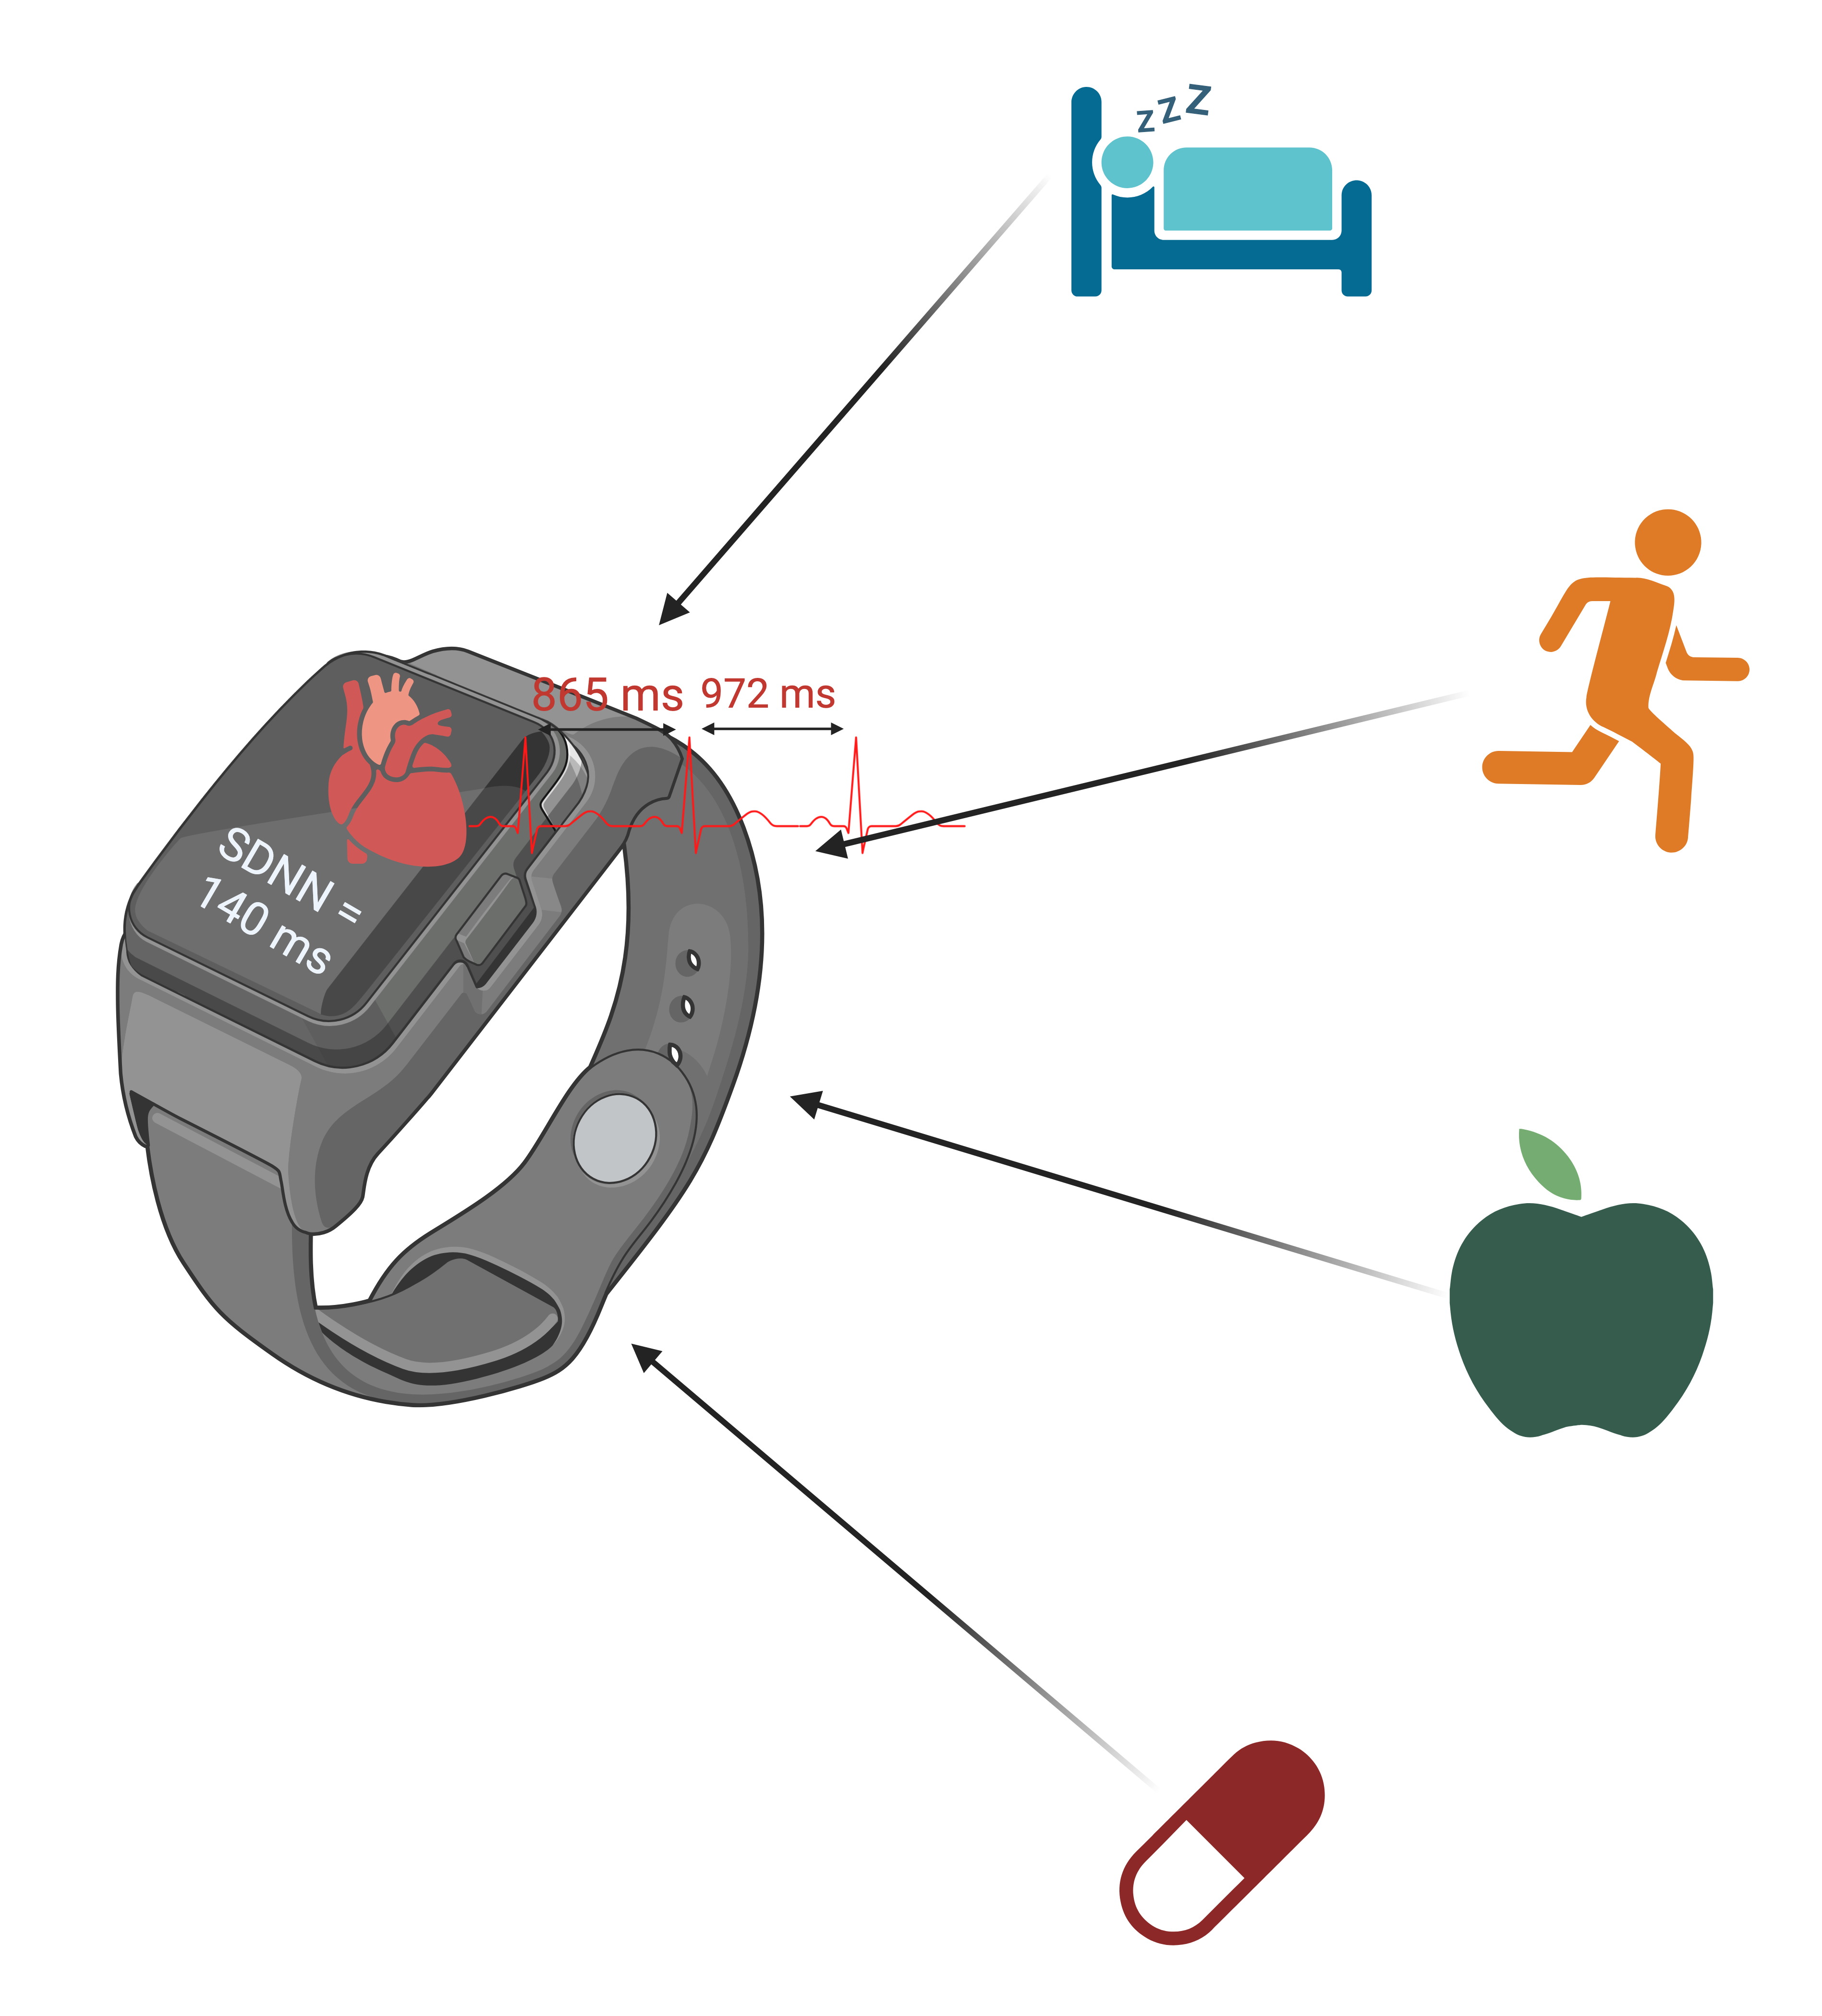
\includegraphics[width=4in,height=\textheight]{images/smartwatch.png}
\emph{(Source: Author)}

}

\caption{\label{fig-smw}\textbf{Hypothetical scenario of lifestyle and
treatment adaptation using HRV in wearable devices}}

\end{figure}

Future research may leverage wearable devices to monitor the
effectiveness of behavioral and pharmacological interventions on HRV at
the individual level. This approach may support precision real-time
monitoring to identify lifestyle patterns or treatments that promote
cardiovascular health through HRV modulation or uncover potential side
effects.\textsuperscript{75}

However, standardization and transparency across wearable device brands
remain a challenge for both research and clinical use. While
smartwatches offer convenient heart rate monitoring, their accuracy
varies due to reliance on photoplethysmography, which can be affected by
motion and other external factors, especially during physical
activity.\textsuperscript{167,168} Despite these limitations, ongoing
improvements in sensor technology and algorithm calibration are likely
to enhance the reliability of wearable-derived HRV and heart rate
data.\textsuperscript{169} Open data formats are important to ensure
that detailed data (e.g., interbeat intervals)\textsuperscript{169,170}
from various devices can be used consistently in health prediction
algorithms, rather than relying only on summarized outputs.

\hypertarget{risk-stratification-1}{%
\section{Risk-stratification}\label{risk-stratification-1}}

The distinct roles of long-term HRV and CART in cardiovascular risk
stratification remain to be fully established. Building on the concept
of continuous monitoring through wearable technology, long-term HRV
presents two promising avenues that warrant further investigation:

\begin{itemize}
\item
  \textbf{Enhancement of existing risk scores:}~HRV may improve the
  predictive accuracy of established cardiovascular risk models, such as
  SCORE2 or the Framingham Risk Score.
\item
  \textbf{Support for treatment decisions:}~Long-term HRV may also help
  optimize the timing of treatment initiation and guide intermediate
  clinical decisions.
\end{itemize}

\emph{Cardiovascular risk assessment}

Digital CVD risk calculators can be used to optimize the timing of
follow-up assessments and treatment initiation. Analyses from Steno
Diabetes Center Copenhagen have suggested that annual retinopathy
screening may not be necessary for all patients. Instead, prediction
models using clinical variables can be used to determine optimal
re-screening intervals.\textsuperscript{171} In prediabetes, a key
concern is overmedicalization, as many individuals do not progress to
T2D or develop complications.\textsuperscript{14} Therefore, efforts to
identify subgroups in prediabetes are needed to enable timely prevention
of cardiovascular complications.\textsuperscript{10} In T2D, data-driven
methods using clinical characteristics have been used to identify who
will benefit most from intensive treatment.\textsuperscript{172} Whether
wearable technologies, such as those measuring HRV, can improve
individualized screening intervals and identify individuals who require
closer clinical attention remains to be investigated.

\emph{Timing and treatment decisions}

In addition to optimizing the timing of follow-up assessments,
cardiovascular risk stratification can also guide when to initiate
treatment. In type 1 diabetes, for example, elevated CVD risk scores are
used to inform decisions about starting lipid-lowering
therapy.\textsuperscript{173} Wearable-derived data may also support
intermediate treatment decisions.\textsuperscript{75} In a UK population
with T2D in clinical practice, patient characteristics have been used to
predict whether SGLT2i or GLP1RA will better improve HbA1c
levels.\textsuperscript{174,175} A further step would be to include
long-term HRV as a clinical characteristic to enhance the prediction of
treatment response. This could enable more precise stratification of
therapy or lifestyle interventions based on the most effective option
for each individual. Whether incorporating long-term HRV into predictive
models can improve the personalization of treatment, particularly for
therapies with cardiovascular effects, remains to be demonstrated. This
conceptual framework may also have potential for guiding the selection
of first-line antihypertensive medications.

As discussed in the clinical implications of CAN in T2D, it remains
unclear how well a CAN diagnosis predicts heart failure risk in the
broader T2D population seen in primary care. Intermediate clinical
decisions are needed for patients diagnosed with CAN to determine
whether to proceed with further evaluation for heart failure using
echocardiography or to initiate specific cardioprotective therapy.

In summary, future research should uncover whether identifying
individuals with high-risk of CVD based on autonomic dysfunction, using
HRV or CAN assessed through CART, can support personalized and timely
cardiovascular screening or interventions.\textsuperscript{75}

\begin{figure}

{\centering 

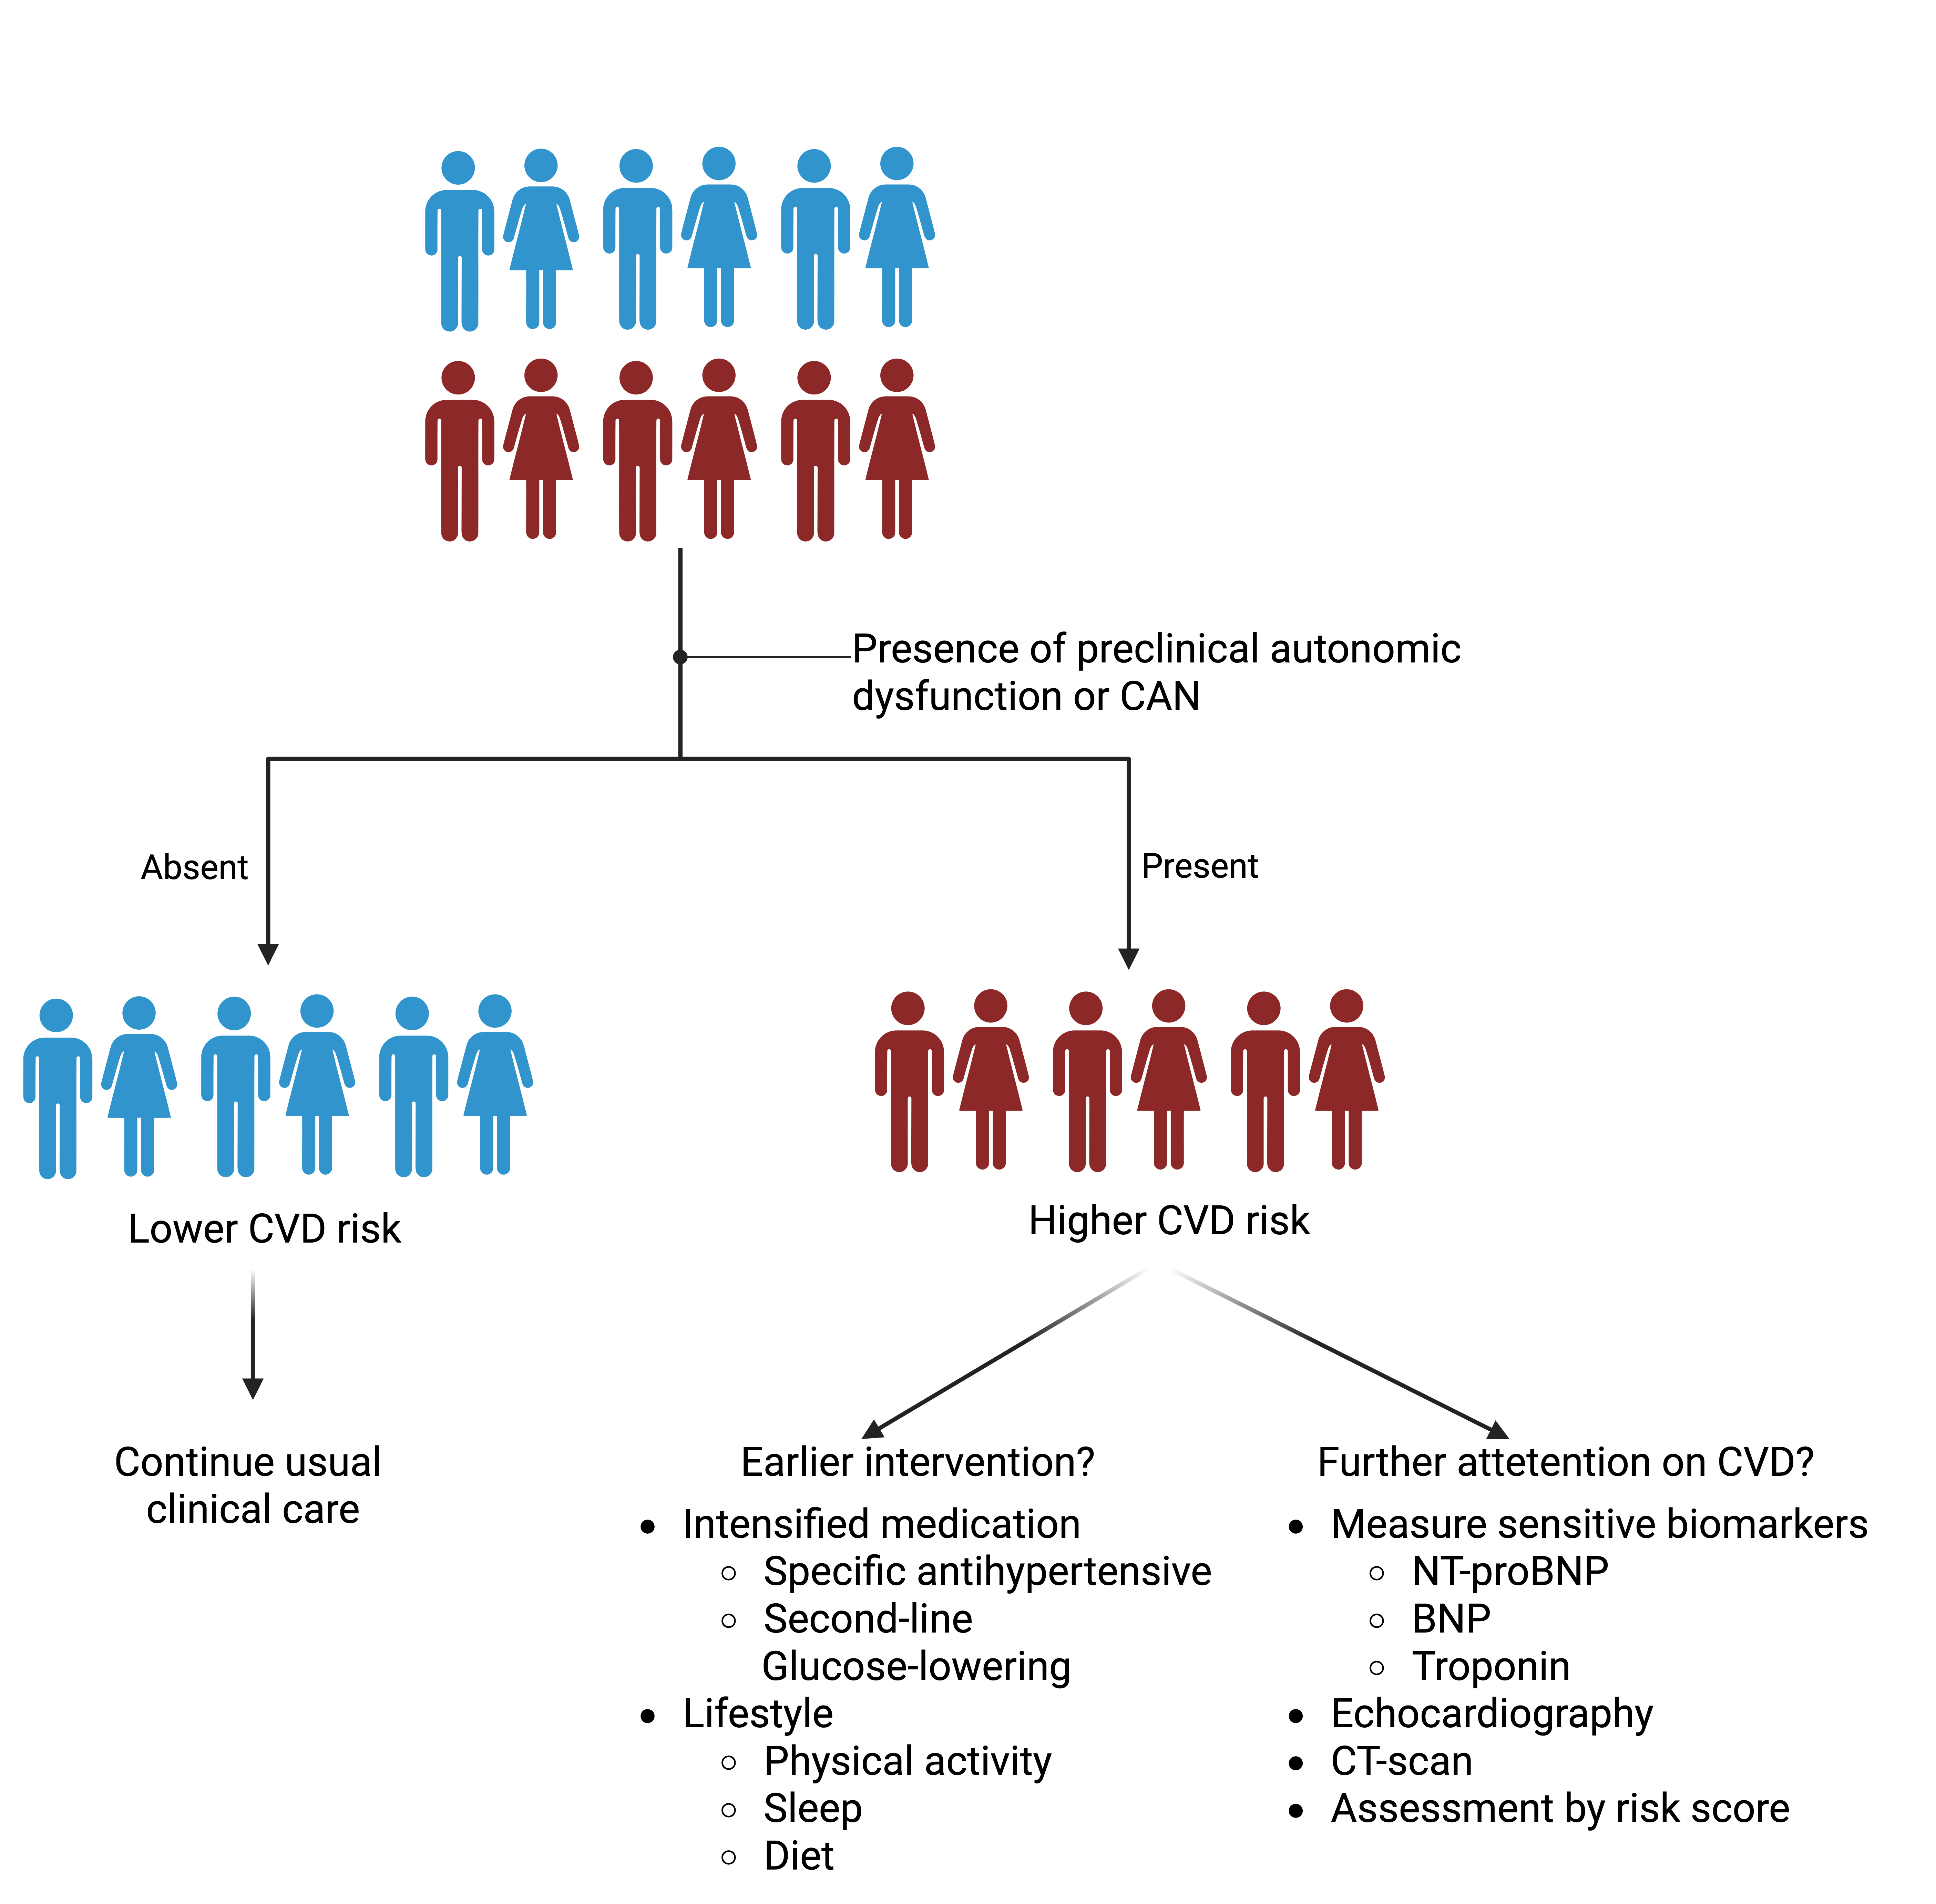
\includegraphics{images/strafication_tree_of_CAN(1).png}\\
\emph{(Source: Author)}

}

\caption{\label{fig-rsp}\textbf{Conceptual model for risk stratification
by autonomic dysfunction}}

\end{figure}

\hypertarget{effective-causal-modifiable-marker}{%
\section{Effective causal modifiable
marker}\label{effective-causal-modifiable-marker}}

The findings support a potential etiological link between long-term HRV
and CVD risk, providing preliminary evidence consistent with a causal
relationship. However, the observed association does not confirm
causality, and further research is needed to determine whether HRV
directly influences CVD outcomes. While randomized controlled trials are
the gold standard for establishing causality, isolating the direct
effect of HRV is particularly challenging. Interventions that affect HRV
often do so indirectly through changes in weight, inflammation, or
insulin sensitivity. Similarly, pharmacological treatments may improve
HRV as a secondary effect, such as through blood pressure reduction from
antihypertensive medications. This makes it difficult to determine
whether modifying HRV itself leads to improved cardiovascular outcomes.

To address these limitations, modern epidemiological methods such as
Mendelian randomization and structured causal mediation analysis offer
promising alternatives. These approaches can be used to infer causality
from observational data and estimate indirect effects using trial data.
Notably, no GWAS has yet investigated the genetic determinants of
long-term HRV. Establishing such associations is essential for
understanding its genetic architecture and for using genetic variants as
unconfounded proxies to assess HRV's causal role in CVD. However, a
challenge arises from findings in short-term HRV, which show
considerable pleiotropy. This may complicate the use of Mendelian
randomization, as the method relies on the assumption of no horizontal
pleiotropy.\textsuperscript{176}

\begin{figure}

{\centering 

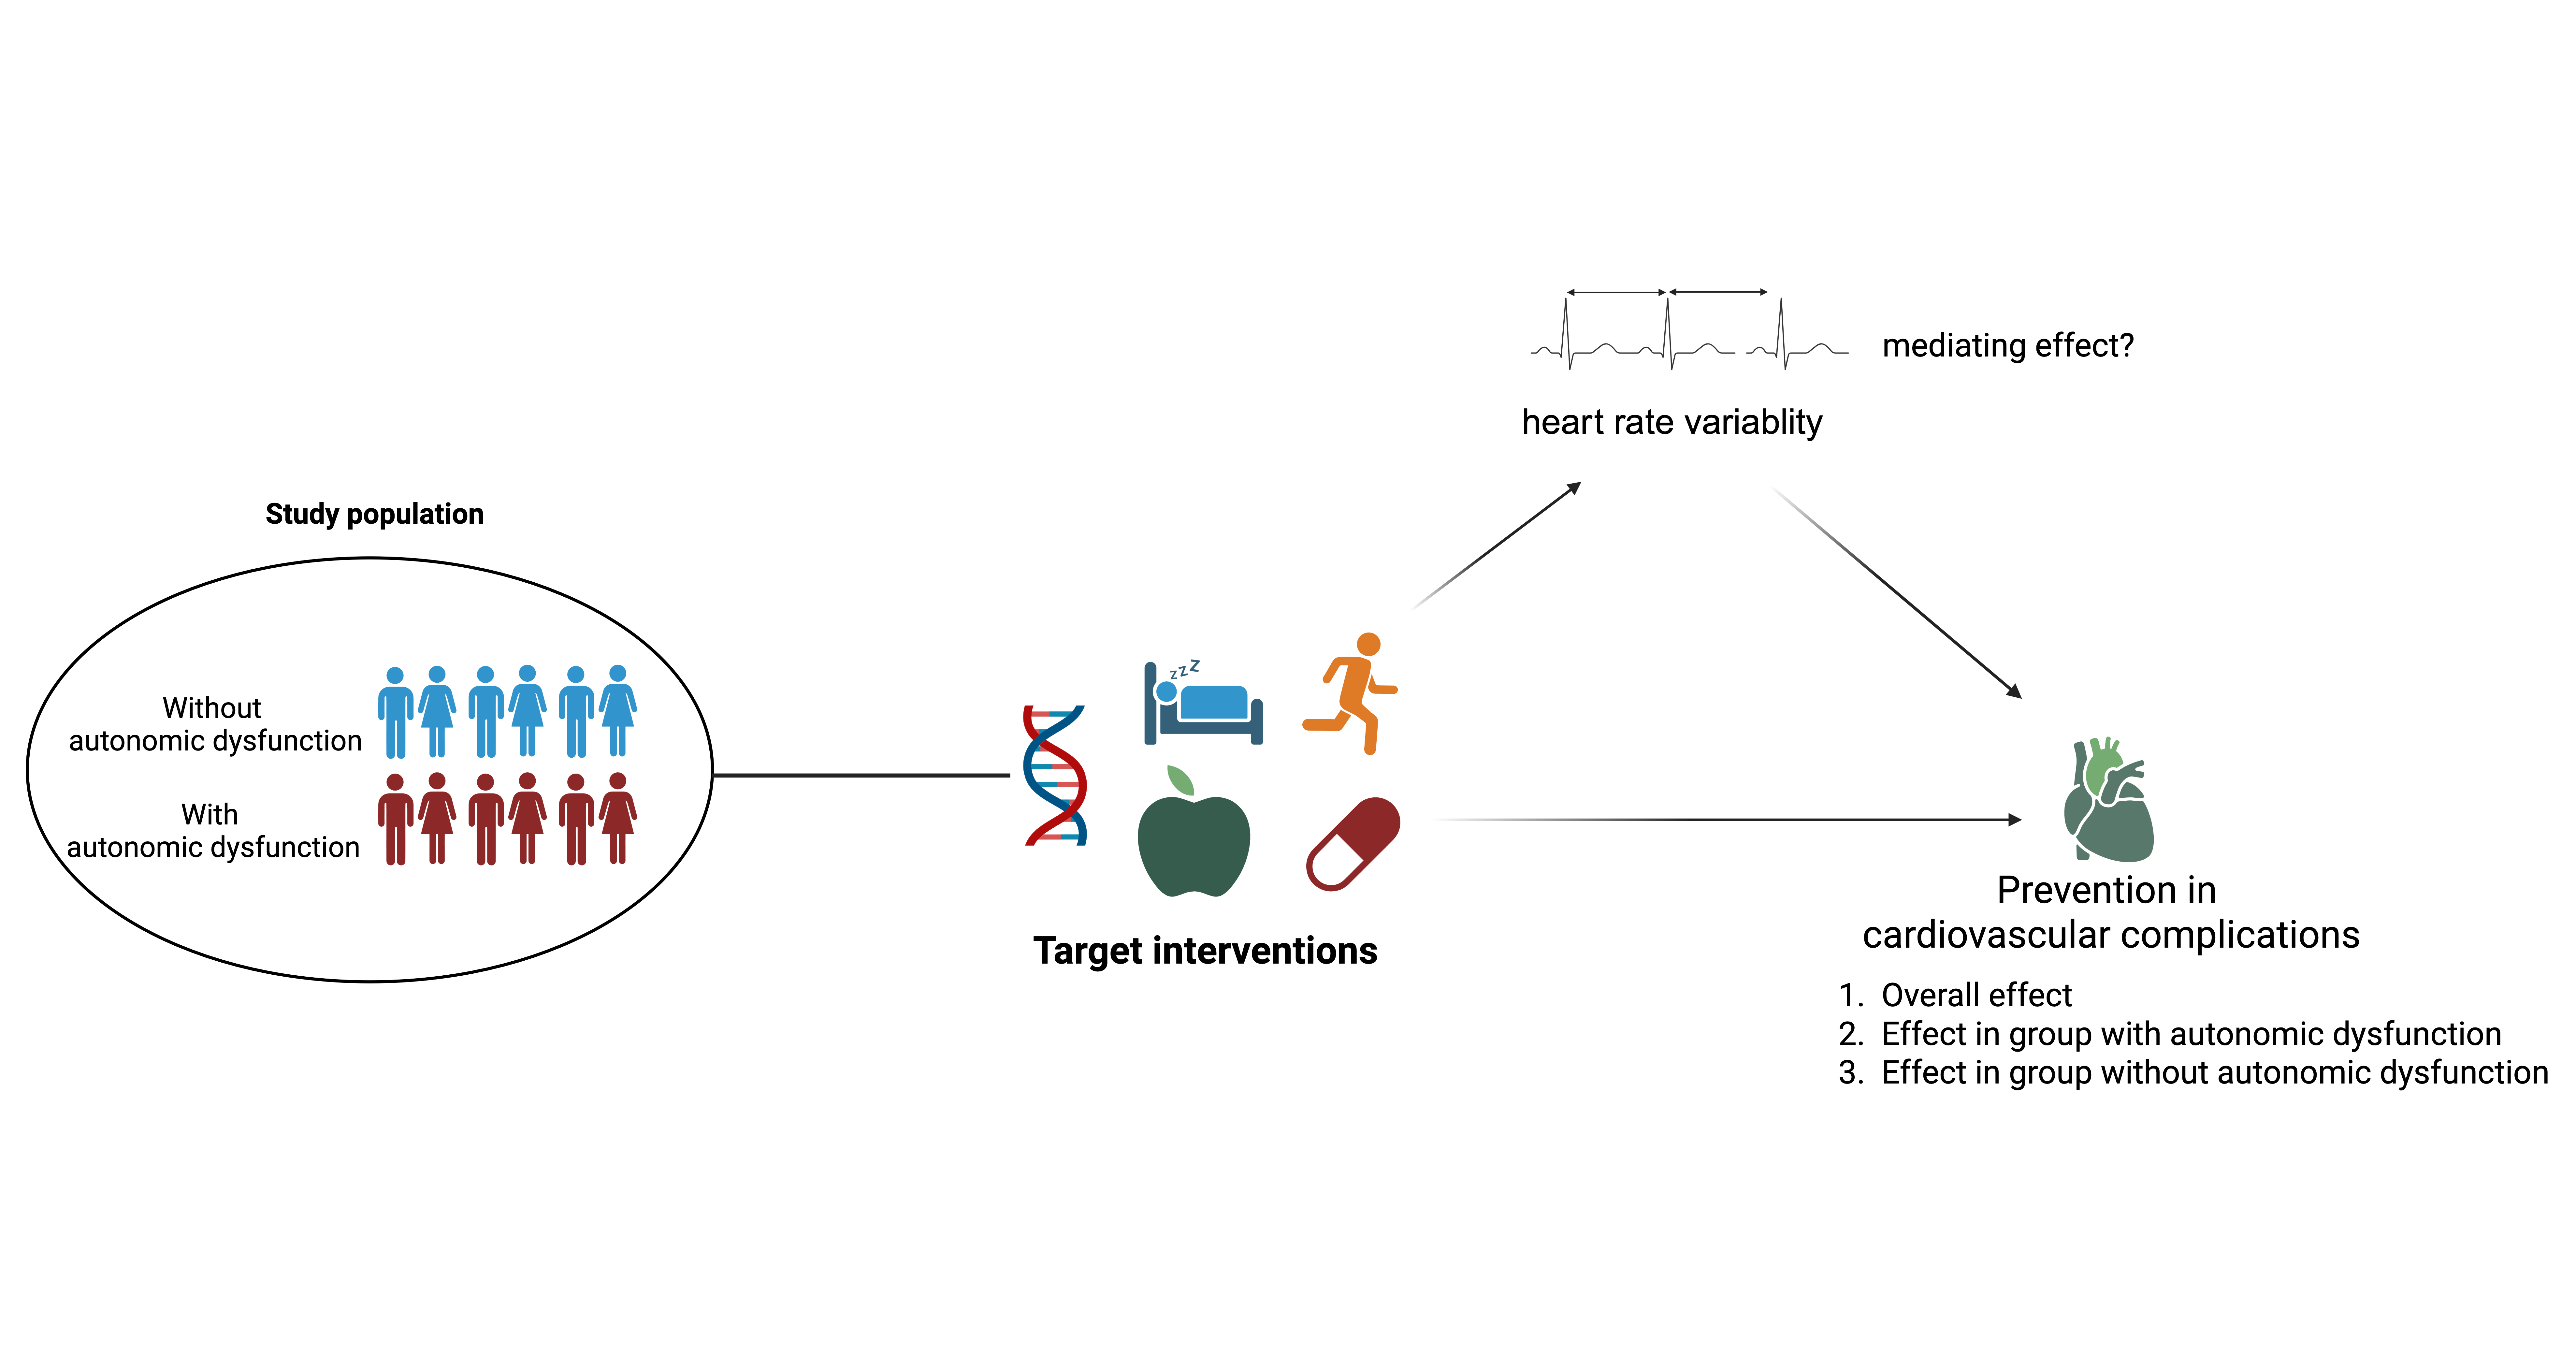
\includegraphics{images/Mediation_HRV_1.png} \emph{(Source: Author)}

}

\caption{\label{fig-mediation}\textbf{Suggested mediation of HRV by
intervention/observation in the prevention of CVD}}

\end{figure}

Future cardiometabolic intervention trials and longitudinal cohorts,
whether focused on lifestyle or pharmacological strategies, should,
where feasible, include repeated HRV measurements.\textsuperscript{77}
In trials, structured mediation analyses are enabled and used to
determine whether modifying autonomic function is associated with
sustained improvements in cardiovascular outcomes. Such evidence could
clarify whether interventions like antihypertensive medications or
lifestyle changes in physical activity, diet, and sleep can causally and
sustainably improve CVD risk through HRV modulation. Using observational
data with repeated measurements, similiar interventions could be
emulated by targeted trails. A further option is to use a CVD polygenic
risk score as the exposure, CVD as the outcome, and HRV as a mediator to
test whether genetic variation in CVD-related traits is mediated through
HRV.\textsuperscript{177}

\clearpage
\null
\thispagestyle{empty}
\clearpage

\bookmarksetup{startatroot}

\hypertarget{conclusion}{%
\chapter{Conclusion}\label{conclusion}}

\clearpage
\null
\thispagestyle{empty}
\clearpage

This dissertation has investigated how autonomic dysfunction, assessed
by HRV and CARTs, is associated with cardiovascular complications across
different stages of glucose metabolism. The findings support the
hypothesis that autonomic dysfunction is an early and independent marker
of cardiovascular risk.

Autonomic dysfunction was associated with higher arterial stiffness not
only in individuals with T2D, but also in those with prediabetes and
normal glucose metabolism. A particularly pronounced association was
observed in individuals with prediabetes, where lower multiday HRV was
linked to a higher risk of cardiovascular disease, heart failure, and
mortality. These findings suggest that autonomic dysfunction may
contribute to cardiovascular complications even before the onset of T2D,
potentially through a modifying effect during the early stages of
dysglycemia. Among individuals with T2D, standardized CARTs identified
those with CAN who had a higher risk of heart failure, even when
asymptomatic and not classified as high risk by risk scores.

Early detection is important, as CVD and heart failure are associated
with reduced life expectancy and quality of life. This dissertation has
demonstrated the potential of autonomic dysfunction as a clinically
relevant marker of cardiovascular risk across the full spectrum of
glucose metabolism, including stages prior to the onset of T2D.

Modern epidemiological methods, e.g.~mediation analysis and Mendelian
randomization, are needed to ascertain causality. Moreover, further
research is needed to determine the clinical utility of long-term HRV
and CARTs in risk stratification, including their potential to timely
initiate individually adapted health assessment or intervention.

\clearpage
\null
\thispagestyle{empty}
\clearpage

\bookmarksetup{startatroot}

\hypertarget{references}{%
\chapter*{References}\label{references}}
\addcontentsline{toc}{chapter}{References}

\markboth{References}{References}

\clearpage
\null
\thispagestyle{empty}
\clearpage

\hypertarget{refs}{}
\begin{CSLReferences}{0}{0}
\leavevmode\vadjust pre{\hypertarget{ref-diabetes2025}{}}%
\CSLLeftMargin{1 }%
\CSLRightInline{International Diabetes Federation. Diabetes atlas, 11th
Edition. International Diabetes Federation, 2025.}

\leavevmode\vadjust pre{\hypertarget{ref-magliano2022}{}}%
\CSLLeftMargin{2 }%
\CSLRightInline{Magliano DJ, Chen L, Carstensen B, \emph{et al.}
\href{https://doi.org/10.1016/S2213-8587(21)00327-2}{Trends in all-cause
mortality among people with diagnosed diabetes in high-income settings:
A multicountry analysis of aggregate data}. \emph{The Lancet Diabetes \&
Endocrinology} 2022; \textbf{10}: 112--9.}

\leavevmode\vadjust pre{\hypertarget{ref-zamana}{}}%
\CSLLeftMargin{3 }%
\CSLRightInline{Zaman S, Wasfy JH, Kapil V, \emph{et al.} The lancet
commission on rethinking coronary artery disease: Moving from ischaemia
to atheroma. \emph{The Lancet}
DOI:\href{https://doi.org/10.1016/S0140-6736(25)00055-8}{10.1016/S0140-6736(25)00055-8}.}

\leavevmode\vadjust pre{\hypertarget{ref-pop-busui2022}{}}%
\CSLLeftMargin{4 }%
\CSLRightInline{Pop-Busui R, Januzzi JL, Bruemmer D, \emph{et al.}
\href{https://doi.org/10.2337/dci22-0014}{Heart failure: An
underappreciated complication of diabetes. A consensus report of the
american diabetes association}. \emph{Diabetes Care} 2022; \textbf{45}:
1670--90.}

\leavevmode\vadjust pre{\hypertarget{ref-hillebrand2013}{}}%
\CSLLeftMargin{5 }%
\CSLRightInline{Hillebrand S, Gast KB, Mutsert R de, \emph{et al.}
\href{https://doi.org/10.1093/europace/eus341}{Heart rate variability
and first cardiovascular event in populations without known
cardiovascular disease: Meta-analysis and dose{\textendash}response
meta-regression}. \emph{EP Europace} 2013; \textbf{15}: 742--9.}

\leavevmode\vadjust pre{\hypertarget{ref-taskforceoftheeuropeansocietyofcardiologythenorthamericansocietyofpacingelectrophysiology1996}{}}%
\CSLLeftMargin{6 }%
\CSLRightInline{Task Force of the European Society of Cardiology the
North American Society of Pacing Electrophysiology.
\href{https://doi.org/doi:10.1161/01.CIR.93.5.1043}{Heart rate
variability}. \emph{Circulation} 1996; \textbf{93}: 1043--65.}

\leavevmode\vadjust pre{\hypertarget{ref-eleftheriadou2024}{}}%
\CSLLeftMargin{7 }%
\CSLRightInline{Eleftheriadou A, Spallone V, Tahrani AA, Alam U.
\href{https://doi.org/10.1007/s00125-024-06242-0}{Cardiovascular
autonomic neuropathy in diabetes: An update with a focus on management}.
\emph{Diabetologia} 2024; \textbf{67}: 2611--25.}

\leavevmode\vadjust pre{\hypertarget{ref-coopmans2020}{}}%
\CSLLeftMargin{8 }%
\CSLRightInline{Coopmans C, Zhou TL, Henry RMA, \emph{et al.}
\href{https://doi.org/10.2337/dc19-2367}{Both prediabetes and type 2
diabetes are associated with lower heart rate variability: The
maastricht study}. \emph{Diabetes Care} 2020; \textbf{43}: 1126--33.}

\leavevmode\vadjust pre{\hypertarget{ref-rooney2023}{}}%
\CSLLeftMargin{9 }%
\CSLRightInline{Rooney MR, Fang M, Ogurtsova K, \emph{et al.}
\href{https://doi.org/10.2337/dc22-2376}{Global prevalence of
prediabetes}. \emph{Diabetes Care} 2023; \textbf{46}: 1388--94.}

\leavevmode\vadjust pre{\hypertarget{ref-birkenfeld2024}{}}%
\CSLLeftMargin{10 }%
\CSLRightInline{Birkenfeld AL, Franks PW, Mohan V.
\href{https://doi.org/10.1161/CIRCULATIONAHA.124.070463}{Precision
medicine in people at risk for diabetes and atherosclerotic
cardiovascular disease: A fresh perspective on prevention}.
\emph{Circulation} 2024; \textbf{150}: 1910--2.}

\leavevmode\vadjust pre{\hypertarget{ref-dhingra2023}{}}%
\CSLLeftMargin{11 }%
\CSLRightInline{Dhingra LS, Aminorroaya A, Oikonomou EK, \emph{et al.}
\href{https://doi.org/10.1001/jamanetworkopen.2023.16634}{Use of
wearable devices in individuals with or at risk for cardiovascular
disease in the US, 2019 to 2020}. \emph{JAMA Network Open} 2023;
\textbf{6}: e2316634--4.}

\leavevmode\vadjust pre{\hypertarget{ref-bayoumy2021}{}}%
\CSLLeftMargin{12 }%
\CSLRightInline{Bayoumy K, Gaber M, Elshafeey A, \emph{et al.}
\href{https://doi.org/10.1038/s41569-021-00522-7}{Smart wearable devices
in cardiovascular care: Where we are and how to move forward}.
\emph{Nature Reviews Cardiology} 2021; \textbf{18}: 581--99.}

\leavevmode\vadjust pre{\hypertarget{ref-natarajan2020}{}}%
\CSLLeftMargin{13 }%
\CSLRightInline{Natarajan A, Pantelopoulos A, Emir-Farinas H, Natarajan
P. \href{https://doi.org/10.1016/S2589-7500(20)30246-6}{Heart rate
variability with photoplethysmography in 8 million individuals: A
cross-sectional study}. \emph{The Lancet Digital Health} 2020;
\textbf{2}: e650--7.}

\leavevmode\vadjust pre{\hypertarget{ref-tabuxe1k2012}{}}%
\CSLLeftMargin{14 }%
\CSLRightInline{Tabák AG, Herder C, Rathmann W, Brunner EJ, Kivimäki M.
\href{https://doi.org/10.1016/S0140-6736(12)60283-9}{Prediabetes: A
high-risk state for diabetes development}. \emph{The Lancet} 2012;
\textbf{379}: 2279--90.}

\leavevmode\vadjust pre{\hypertarget{ref-bonora2018}{}}%
\CSLLeftMargin{15 }%
\CSLRightInline{Bonora E, DeFronzo R. Diabetes. Epidemiology, genetics,
pathogenesis, diagnosis, prevention, and treatment. 2018
DOI:\href{https://doi.org/10.1007/978-3-319-27317-4}{10.1007/978-3-319-27317-4}.}

\leavevmode\vadjust pre{\hypertarget{ref-worldhealthorganization2020}{}}%
\CSLLeftMargin{16 }%
\CSLRightInline{World Health Organization. Diagnosis and management of
type 2 diabetes (HEARTS-d). Geneva, 2020.}

\leavevmode\vadjust pre{\hypertarget{ref-americandiabetesassociationprofessionalpracticecommittee2021}{}}%
\CSLLeftMargin{17 }%
\CSLRightInline{American Diabetes Association Professional Practice
Committee. \href{https://doi.org/10.2337/dc22-S002}{2. Classification
and diagnosis of diabetes: Standards of medical care in
diabetes{\textemdash}2022}. \emph{Diabetes Care} 2021; \textbf{45}:
S17--38.}

\leavevmode\vadjust pre{\hypertarget{ref-colagiuri2010}{}}%
\CSLLeftMargin{18 }%
\CSLRightInline{Colagiuri S, Lee CMY, Wong TY, \emph{et al.}
\href{https://doi.org/10.2337/dc10-1206}{Glycemic thresholds for
diabetes-specific retinopathy: Implications for diagnostic criteria for
diabetes}. \emph{Diabetes Care} 2010; \textbf{34}: 145--50.}

\leavevmode\vadjust pre{\hypertarget{ref-mokhtar2023}{}}%
\CSLLeftMargin{19 }%
\CSLRightInline{Mokhtar SBA, Heide FCT van der, Oyaert KAM, \emph{et
al.} \href{https://doi.org/10.1007/s00125-023-05986-5}{(Pre)diabetes and
a higher level of glycaemic measures are continuously associated with
corneal neurodegeneration assessed by corneal confocal microscopy: The
maastricht study}. \emph{Diabetologia} 2023; \textbf{66}: 2030--41.}

\leavevmode\vadjust pre{\hypertarget{ref-huang2014}{}}%
\CSLLeftMargin{20 }%
\CSLRightInline{Huang Y, Cai X, Qiu M, \emph{et al.}
\href{https://doi.org/10.1007/s00125-014-3361-2}{Prediabetes and the
risk of cancer: A meta-analysis}. \emph{Diabetologia} 2014; \textbf{57}:
2261--9.}

\leavevmode\vadjust pre{\hypertarget{ref-stehouwer2018}{}}%
\CSLLeftMargin{21 }%
\CSLRightInline{Stehouwer CDA.
\href{https://doi.org/10.2337/dbi17-0044}{Microvascular dysfunction and
hyperglycemia: A vicious cycle with widespread consequences}.
\emph{Diabetes} 2018; \textbf{67}: 1729--41.}

\leavevmode\vadjust pre{\hypertarget{ref-taylor2013}{}}%
\CSLLeftMargin{22 }%
\CSLRightInline{Taylor R. \href{https://doi.org/10.2337/dc12-1805}{Type
2 diabetes: Etiology and reversibility}. \emph{Diabetes Care} 2013;
\textbf{36}: 1047--55.}

\leavevmode\vadjust pre{\hypertarget{ref-fuxe6rch2013}{}}%
\CSLLeftMargin{23 }%
\CSLRightInline{Færch K, Witte DR, Tabák AG, \emph{et al.}
\href{https://doi.org/10.1016/S2213-8587(13)70008-1}{Trajectories of
cardiometabolic risk factors before diagnosis of three subtypes of type
2 diabetes: a post-hoc analysis of the longitudinal Whitehall II cohort
study.} \emph{The lancet Diabetes \& endocrinology} 2013; \textbf{1}:
43--51.}

\leavevmode\vadjust pre{\hypertarget{ref-ritchie2020}{}}%
\CSLLeftMargin{24 }%
\CSLRightInline{Ritchie RH, Abel ED.
\href{https://doi.org/10.1161/CIRCRESAHA.120.315913}{Basic mechanisms of
diabetic heart disease}. \emph{Circulation Research} 2020; \textbf{126}:
1501--25.}

\leavevmode\vadjust pre{\hypertarget{ref-yusuf2020}{}}%
\CSLLeftMargin{25 }%
\CSLRightInline{Yusuf S, Joseph P, Rangarajan S, \emph{et al.}
\href{https://doi.org/10.1016/S0140-6736(19)32008-2}{Modifiable risk
factors, cardiovascular disease, and mortality in 155{\hphantom{,}}722
individuals from 21 high-income, middle-income, and low-income countries
(PURE): A prospective cohort study}. \emph{The Lancet} 2020;
\textbf{395}: 795--808.}

\leavevmode\vadjust pre{\hypertarget{ref-wood2001}{}}%
\CSLLeftMargin{26 }%
\CSLRightInline{Wood D.
\href{https://doi.org/10.1067/mhj.2001.109951}{Established and emerging
cardiovascular risk factors}. \emph{American Heart Journal} 2001;
\textbf{141}: S49--57.}

\leavevmode\vadjust pre{\hypertarget{ref-moore2019}{}}%
\CSLLeftMargin{27 }%
\CSLRightInline{Moore KJ.
\href{https://doi.org/10.1038/s41569-018-0144-3}{Targeting inflammation
in CVD: Advances and challenges}. \emph{Nature Reviews Cardiology} 2019;
\textbf{16}: 74--5.}

\leavevmode\vadjust pre{\hypertarget{ref-fuchs2020}{}}%
\CSLLeftMargin{28 }%
\CSLRightInline{Fuchs FD, Whelton PK.
\href{https://doi.org/10.1161/HYPERTENSIONAHA.119.14240}{High blood
pressure and cardiovascular disease}. \emph{Hypertension} 2020;
\textbf{75}: 285--92.}

\leavevmode\vadjust pre{\hypertarget{ref-mitchell2020}{}}%
\CSLLeftMargin{29 }%
\CSLRightInline{Mitchell GF, Powell JT.
\href{https://doi.org/10.1161/ATVBAHA.120.314208}{Arteriosclerosis}.
\emph{Arteriosclerosis, Thrombosis, and Vascular Biology} 2020;
\textbf{40}: 1025--7.}

\leavevmode\vadjust pre{\hypertarget{ref-florea2014}{}}%
\CSLLeftMargin{30 }%
\CSLRightInline{Florea VG, Cohn JN.
\href{https://doi.org/10.1161/CIRCRESAHA.114.302589}{The autonomic
nervous system and heart failure}. \emph{Circulation Research} 2014;
\textbf{114}: 1815--26.}

\leavevmode\vadjust pre{\hypertarget{ref-mancia2014}{}}%
\CSLLeftMargin{31 }%
\CSLRightInline{Mancia G, Grassi G.
\href{https://doi.org/10.1161/CIRCRESAHA.114.302524}{The autonomic
nervous system and hypertension}. \emph{Circulation Research} 2014;
\textbf{114}: 1804--14.}

\leavevmode\vadjust pre{\hypertarget{ref-ziegler2025}{}}%
\CSLLeftMargin{32 }%
\CSLRightInline{Ziegler KA, Engelhardt S, Carnevale D, \emph{et al.}
\href{https://doi.org/10.1161/CIRCRESAHA.125.325580}{Neural mechanisms
in cardiovascular health and disease}. \emph{Circulation Research} 2025;
\textbf{136}: 1233--61.}

\leavevmode\vadjust pre{\hypertarget{ref-wagner2023}{}}%
\CSLLeftMargin{33 }%
\CSLRightInline{Wagner JUG, Tombor LS, Malacarne PF, \emph{et al.}
\href{https://doi.org/10.1126/science.ade4961}{Aging impairs the
neurovascular interface in the heart}. \emph{Science} 2023;
\textbf{381}: 897--906.}

\leavevmode\vadjust pre{\hypertarget{ref-lee2010}{}}%
\CSLLeftMargin{34 }%
\CSLRightInline{Lee H-Y, Oh B-H.
\href{https://doi.org/10.1253/circj.CJ-10-0910}{Aging and arterial
stiffness}. \emph{Circulation Journal} 2010; \textbf{74}: 2257--62.}

\leavevmode\vadjust pre{\hypertarget{ref-lu2023}{}}%
\CSLLeftMargin{35 }%
\CSLRightInline{Lu Y, Kiechl SJ, Wang J, Xu Q, Kiechl S, Pechlaner R.
\href{https://doi.org/10.1016/j.ebiom.2023.104619}{Global distributions
of age- and sex-related arterial stiffness: systematic review and
meta-analysis of 167 studies with 509,743 participants}.
\emph{EBioMedicine} 2023; \textbf{92}: 104619.}

\leavevmode\vadjust pre{\hypertarget{ref-zhong2018}{}}%
\CSLLeftMargin{36 }%
\CSLRightInline{Zhong Q, Hu M-J, Cui Y-J, \emph{et al.}
\href{https://doi.org/10.1177/0003319717742544}{Carotid{\textendash}femoral
pulse wave velocity in the prediction of cardiovascular events and
mortality: An updated systematic review and meta-analysis}.
\emph{Angiology} 2018; \textbf{69}: 617--29.}

\leavevmode\vadjust pre{\hypertarget{ref-libby2021}{}}%
\CSLLeftMargin{37 }%
\CSLRightInline{Libby P.
\href{https://doi.org/10.1038/s41586-021-03392-8}{The changing landscape
of atherosclerosis}. \emph{Nature} 2021; \textbf{592}: 524--33.}

\leavevmode\vadjust pre{\hypertarget{ref-zaman}{}}%
\CSLLeftMargin{38 }%
\CSLRightInline{Zaman S, Wasfy JH, Kapil V, \emph{et al.} The lancet
commission on rethinking coronary artery disease: Moving from ischaemia
to atheroma. \emph{The Lancet}
DOI:\href{https://doi.org/10.1016/S0140-6736(25)00055-8}{10.1016/S0140-6736(25)00055-8}.}

\leavevmode\vadjust pre{\hypertarget{ref-kawai2024}{}}%
\CSLLeftMargin{39 }%
\CSLRightInline{Kawai K, Kawakami R, Finn AV, Virmani R.
\href{https://doi.org/10.1161/ATVBAHA.124.319396}{Differences in stable
and unstable atherosclerotic plaque}. \emph{Arteriosclerosis,
Thrombosis, and Vascular Biology} 2024; \textbf{44}: 1474--84.}

\leavevmode\vadjust pre{\hypertarget{ref-alasady2013}{}}%
\CSLLeftMargin{40 }%
\CSLRightInline{Alasady M, Shipp NJ, Brooks AG, \emph{et al.}
\href{https://doi.org/10.1161/CIRCEP.113.000163}{Myocardial infarction
and atrial fibrillation}. \emph{Circulation: Arrhythmia and
Electrophysiology} 2013; \textbf{6}: 738--45.}

\leavevmode\vadjust pre{\hypertarget{ref-elgendy2019}{}}%
\CSLLeftMargin{41 }%
\CSLRightInline{Elgendy IY, Mahtta D, Pepine CJ.
\href{https://doi.org/10.1161/CIRCRESAHA.118.313568}{Medical therapy for
heart failure caused by ischemic heart disease}. \emph{Circulation
Research} 2019; \textbf{124}: 1520--35.}

\leavevmode\vadjust pre{\hypertarget{ref-thygesen2018}{}}%
\CSLLeftMargin{42 }%
\CSLRightInline{Thygesen K, Alpert JS, Jaffe AS, \emph{et al.}
\href{https://doi.org/10.1161/CIR.0000000000000617}{Fourth universal
definition of myocardial infarction (2018)}. \emph{Circulation} 2018;
\textbf{138}: e618--51.}

\leavevmode\vadjust pre{\hypertarget{ref-cherla2024}{}}%
\CSLLeftMargin{43 }%
\CSLRightInline{Cherla A, Kyriopoulos I, Pearcy P, \emph{et al.} Trends
in avoidable mortality from cardiovascular diseases in the european
union, 1995{\textendash}2020: A retrospective secondary data analysis.
\emph{The Lancet Regional Health {\textendash} Europe} 2024;
\textbf{47}.
DOI:\href{https://doi.org/10.1016/j.lanepe.2024.101079}{10.1016/j.lanepe.2024.101079}.}

\leavevmode\vadjust pre{\hypertarget{ref-bilano2015}{}}%
\CSLLeftMargin{44 }%
\CSLRightInline{Bilano V, Gilmour S, Moffiet T, \emph{et al.}
\href{https://doi.org/10.1016/S0140-6736(15)60264-1}{Global trends and
projections for tobacco use, 1990{\textendash}2025: An analysis of
smoking indicators from the WHO comprehensive information systems for
tobacco control}. \emph{The Lancet} 2015; \textbf{385}: 966--76.}

\leavevmode\vadjust pre{\hypertarget{ref-ockene1997}{}}%
\CSLLeftMargin{45 }%
\CSLRightInline{Ockene IS, Miller NH.
\href{https://doi.org/10.1161/01.CIR.96.9.3243}{Cigarette smoking,
cardiovascular disease, and stroke}. \emph{Circulation} 1997;
\textbf{96}: 3243--7.}

\leavevmode\vadjust pre{\hypertarget{ref-wallentin2014}{}}%
\CSLLeftMargin{46 }%
\CSLRightInline{Wallentin L, Kristensen SD, Anderson JL, \emph{et al.}
\href{https://doi.org/10.1016/j.ahj.2014.07.006}{How can we optimize the
processes of care for acute coronary syndromes to improve outcomes?}
\emph{American Heart Journal} 2014; \textbf{168}: 622--631.e2.}

\leavevmode\vadjust pre{\hypertarget{ref-shah2015}{}}%
\CSLLeftMargin{47 }%
\CSLRightInline{Shah AD, Langenberg C, Rapsomaniki E, \emph{et al.}
\href{https://doi.org/10.1016/S2213-8587(14)70219-0}{Type 2 diabetes and
incidence of cardiovascular diseases: A cohort study in 1·9 million
people}. \emph{The Lancet Diabetes \& Endocrinology} 2015; \textbf{3}:
105--13.}

\leavevmode\vadjust pre{\hypertarget{ref-glynn2024}{}}%
\CSLLeftMargin{48 }%
\CSLRightInline{Glynn L, Lind M, Andersson T, Eliasson B, Hofmann R,
Nyström T. \href{https://doi.org/10.1161/JAHA.123.034741}{Trends in
survival after first myocardial infarction in people with diabetes}.
\emph{Journal of the American Heart Association} 2024; \textbf{13}:
e034741.}

\leavevmode\vadjust pre{\hypertarget{ref-greggedwardw.a}{}}%
\CSLLeftMargin{49 }%
\CSLRightInline{Gregg Edward W., Li Yanfeng, Wang Jing, \emph{et al.}
\href{https://doi.org/10.1056/NEJMoa1310799}{Changes in diabetes-related
complications in the united states, 1990{\textendash}2010}. \emph{New
England Journal of Medicine}; \textbf{370}: 1514--23.}

\leavevmode\vadjust pre{\hypertarget{ref-campbell2019}{}}%
\CSLLeftMargin{50 }%
\CSLRightInline{Campbell BCV, De Silva DA, Macleod MR, \emph{et al.}
\href{https://doi.org/10.1038/s41572-019-0118-8}{Ischaemic stroke}.
\emph{Nature Reviews Disease Primers} 2019; \textbf{5}: 70.}

\leavevmode\vadjust pre{\hypertarget{ref-magid-bernstein2022}{}}%
\CSLLeftMargin{51 }%
\CSLRightInline{Magid-Bernstein J, Girard R, Polster S, \emph{et al.}
\href{https://doi.org/10.1161/CIRCRESAHA.121.319949}{Cerebral
hemorrhage: Pathophysiology, treatment, and future directions}.
\emph{Circulation Research} 2022; \textbf{130}: 1204--29.}

\leavevmode\vadjust pre{\hypertarget{ref-donnan2008}{}}%
\CSLLeftMargin{52 }%
\CSLRightInline{Donnan GA, Fisher M, Macleod M, Davis SM.
\href{https://doi.org/10.1016/S0140-6736(08)60694-7}{Stroke}. \emph{The
Lancet} 2008; \textbf{371}: 1612--23.}

\leavevmode\vadjust pre{\hypertarget{ref-vos2020}{}}%
\CSLLeftMargin{53 }%
\CSLRightInline{Vos T, Lim SS, Abbafati C, \emph{et al.}
\href{https://doi.org/10.1016/S0140-6736(20)30925-9}{Global burden of
369 diseases and injuries in 204 countries and territories,
1990{\textendash}2019: A systematic analysis for the global burden of
disease study 2019}. \emph{The Lancet} 2020; \textbf{396}: 1204--22.}

\leavevmode\vadjust pre{\hypertarget{ref-li2024}{}}%
\CSLLeftMargin{54 }%
\CSLRightInline{Li X, Kong X, Yang C, \emph{et al.} Global, regional,
and national burden of ischemic stroke, 1990{\textendash}2021: An
analysis of data from the global burden of disease study 2021.
\emph{eClinicalMedicine} 2024; \textbf{75}.
DOI:\href{https://doi.org/10.1016/j.eclinm.2024.102758}{10.1016/j.eclinm.2024.102758}.}

\leavevmode\vadjust pre{\hypertarget{ref-lee2012}{}}%
\CSLLeftMargin{55 }%
\CSLRightInline{Lee M, Saver JL, Hong K-S, Song S, Chang K-H, Ovbiagele
B. \href{https://doi.org/10.1136/bmj.e3564}{Effect of pre-diabetes on
future risk of stroke: Meta-analysis}. \emph{BMJ : British Medical
Journal} 2012; \textbf{344}: e3564.}

\leavevmode\vadjust pre{\hypertarget{ref-barr2007}{}}%
\CSLLeftMargin{56 }%
\CSLRightInline{Barr ELM, Zimmet PZ, Welborn TA, \emph{et al.}
\href{https://doi.org/10.1161/CIRCULATIONAHA.106.685628}{Risk of
cardiovascular and all-cause mortality in individuals with diabetes
mellitus, impaired fasting glucose, and impaired glucose tolerance}.
\emph{Circulation} 2007; \textbf{116}: 151--7.}

\leavevmode\vadjust pre{\hypertarget{ref-khan2024}{}}%
\CSLLeftMargin{57 }%
\CSLRightInline{Khan MS, Shahid I, Bennis A, Rakisheva A, Metra M,
Butler J. \href{https://doi.org/10.1038/s41569-024-01046-6}{Global
epidemiology of heart failure}. \emph{Nature Reviews Cardiology} 2024;
\textbf{21}: 717--34.}

\leavevmode\vadjust pre{\hypertarget{ref-heidenreich2022}{}}%
\CSLLeftMargin{58 }%
\CSLRightInline{Heidenreich PA, Bozkurt B, Aguilar D, \emph{et al.}
\href{https://doi.org/10.1161/CIR.0000000000001063}{2022 AHA/ACC/HFSA
guideline for the management of heart failure: A report of the american
college of cardiology/american heart association joint committee on
clinical practice guidelines}. \emph{Circulation} 2022; \textbf{145}:
e895--1032.}

\leavevmode\vadjust pre{\hypertarget{ref-campbell2024}{}}%
\CSLLeftMargin{59 }%
\CSLRightInline{Campbell P, Rutten FH, Lee MM, Hawkins NM, Petrie MC.
\href{https://doi.org/10.1016/S0140-6736(23)02756-3}{Heart failure with
preserved ejection fraction: everything the clinician needs to know.}
\emph{Lancet (London, England)} 2024; \textbf{403}: 1083--92.}

\leavevmode\vadjust pre{\hypertarget{ref-normand2019}{}}%
\CSLLeftMargin{60 }%
\CSLRightInline{Normand C, Kaye DM, Povsic TJ, Dickstein K.
\href{https://doi.org/10.1016/S0140-6736(18)32216-5}{Beyond
pharmacological treatment: An insight into therapies that target
specific aspects of heart failure pathophysiology}. \emph{The Lancet}
2019; \textbf{393}: 1045--55.}

\leavevmode\vadjust pre{\hypertarget{ref-schlaich2015}{}}%
\CSLLeftMargin{61 }%
\CSLRightInline{Schlaich M, Straznicky N, Lambert E, Lambert G.
\href{https://doi.org/10.1016/s2213-8587(14)70033-6}{Metabolic syndrome:
a sympathetic disease?} \emph{Lancet Diabetes Endocrinol} 2015;
\textbf{3}: 148--57.}

\leavevmode\vadjust pre{\hypertarget{ref-rinaldi2023}{}}%
\CSLLeftMargin{62 }%
\CSLRightInline{Rinaldi E, Heide FCT van der, Bonora E, \emph{et al.}
\href{https://doi.org/10.1186/s12933-023-01837-0}{Lower heart rate
variability, an index of worse autonomic function, is associated with
worse beta cell response to a glycemic load in vivo{\textemdash}the
maastricht study}. \emph{Cardiovascular Diabetology} 2023; \textbf{22}:
105.}

\leavevmode\vadjust pre{\hypertarget{ref-mahinchowdhury2021}{}}%
\CSLLeftMargin{63 }%
\CSLRightInline{Mahin Chowdhury, Sarah Nevitt, Aikaterini Eleftheriadou,
\emph{et al.} \href{https://doi.org/10.1136/bmjdrc-2021-002480}{Cardiac
autonomic neuropathy and risk of cardiovascular disease and mortality in
type 1 and type 2 diabetes: A meta-analysis}. \emph{BMJ Open Diabetes
Research \& Care} 2021; \textbf{9}: e002480.}

\leavevmode\vadjust pre{\hypertarget{ref-tang2023}{}}%
\CSLLeftMargin{64 }%
\CSLRightInline{Tang Y, Ang L, Jaiswal M, \emph{et al.}
\href{https://doi.org/10.2337/db23-0247}{Cardiovascular autonomic
neuropathy and risk of kidney function decline in type 1 and type 2
diabetes: Findings from the PERL and ACCORD cohorts}. \emph{Diabetes}
2023; \textbf{73}: 751--62.}

\leavevmode\vadjust pre{\hypertarget{ref-immanuel2023}{}}%
\CSLLeftMargin{65 }%
\CSLRightInline{Immanuel S, Teferra MN, Baumert M, Bidargaddi N.
\href{https://doi.org/10.1159/000530376}{Heart rate variability for
evaluating psychological stress changes in healthy adults: A scoping
review}. \emph{Neuropsychobiology} 2023; \textbf{82}: 187--202.}

\leavevmode\vadjust pre{\hypertarget{ref-dong2016}{}}%
\CSLLeftMargin{66 }%
\CSLRightInline{Dong J-G.
\href{https://doi.org/10.3892/etm.2016.3104}{The role of heart rate
variability in sports physiology (review)}. \emph{Experimental and
Therapeutic Medicine} 2016; \textbf{11}: 1531--6.}

\leavevmode\vadjust pre{\hypertarget{ref-singh1996}{}}%
\CSLLeftMargin{67 }%
\CSLRightInline{Singh N, Mironov D, Armstrong PW, Ross AM, Langer A.
\href{https://doi.org/10.1161/01.CIR.93.7.1388}{Heart rate variability
assessment early after acute myocardial infarction}. \emph{Circulation}
1996; \textbf{93}: 1388--95.}

\leavevmode\vadjust pre{\hypertarget{ref-huggett2003}{}}%
\CSLLeftMargin{68 }%
\CSLRightInline{Huggett RJ, Scott EM, Gilbey SG, Stoker JB, Mackintosh
AF, Mary DASG.
\href{https://doi.org/10.1161/01.CIR.0000103123.66264.FE}{Impact of type
2 diabetes mellitus on sympathetic neural mechanisms in hypertension}.
\emph{Circulation} 2003; \textbf{108}: 3097--101.}

\leavevmode\vadjust pre{\hypertarget{ref-cseh2020}{}}%
\CSLLeftMargin{69 }%
\CSLRightInline{Cseh D, Climie RE, Offredo L, \emph{et al.}
\href{https://doi.org/10.1161/ATVBAHA.120.314102}{Type 2 diabetes
mellitus is independently associated with decreased neural baroreflex
sensitivity}. \emph{Arteriosclerosis, Thrombosis, and Vascular Biology}
2020; \textbf{40}: 1420--8.}

\leavevmode\vadjust pre{\hypertarget{ref-hansen2025}{}}%
\CSLLeftMargin{70 }%
\CSLRightInline{Hansen CS, Christensen MMB, Vistisen D, \emph{et al.}
\href{https://doi.org/10.1007/s10286-024-01069-6}{Normative data on
measures of cardiovascular autonomic neuropathy and the effect of
pretest conditions in a large danish non-diabetic CVD-free population
from the lolland-falster health study}. \emph{Clinical Autonomic
Research} 2025; \textbf{35}: 101--13.}

\leavevmode\vadjust pre{\hypertarget{ref-davis2024}{}}%
\CSLLeftMargin{71 }%
\CSLRightInline{Davis TME, Tan E, Davis WA.
\href{https://doi.org/10.1186/s12933-024-02185-3}{Prevalence and
prognostic significance of cardiac autonomic neuropathy in
community-based people with type 2 diabetes: The fremantle diabetes
study phase II}. \emph{Cardiovascular Diabetology} 2024; \textbf{23}:
102.}

\leavevmode\vadjust pre{\hypertarget{ref-davies2022}{}}%
\CSLLeftMargin{72 }%
\CSLRightInline{Davies MJ, Aroda VR, Collins BS, \emph{et al.}
\href{https://doi.org/10.2337/dci22-0034}{Management of hyperglycemia in
type 2 diabetes, 2022. A consensus report by the american diabetes
association (ADA) and the european association for the study of diabetes
(EASD)}. \emph{Diabetes Care} 2022; \textbf{45}: 2753--86.}

\leavevmode\vadjust pre{\hypertarget{ref-reductio2002}{}}%
\CSLLeftMargin{73 }%
\CSLRightInline{\href{https://doi.org/10.1056/NEJMoa012512}{Reduction in
the incidence of type 2 diabetes with lifestyle intervention or
metformin}. \emph{New England Journal of Medicine} 2002; \textbf{346}:
393--403.}

\leavevmode\vadjust pre{\hypertarget{ref-kahn2024}{}}%
\CSLLeftMargin{74 }%
\CSLRightInline{Kahn SE, Deanfield JE, Jeppesen OK, \emph{et al.}
\href{https://doi.org/10.2337/dc24-0491}{Effect of semaglutide on
regression and progression of glycemia in people with overweight or
obesity but without diabetes in the SELECT trial}. \emph{Diabetes Care}
2024; \textbf{47}: 1350--9.}

\leavevmode\vadjust pre{\hypertarget{ref-franks2023}{}}%
\CSLLeftMargin{75 }%
\CSLRightInline{Franks PW, Cefalu WT, Dennis J, \emph{et al.}
\href{https://doi.org/10.1016/s2213-8587(23)00165-1}{Precision medicine
for cardiometabolic disease: a framework for clinical translation}.
\emph{Lancet Diabetes Endocrinol} 2023; \textbf{11}: 822--35.}

\leavevmode\vadjust pre{\hypertarget{ref-schram2014}{}}%
\CSLLeftMargin{76 }%
\CSLRightInline{Schram MT, Sep SJS, Kallen CJ van der, \emph{et al.}
\href{https://doi.org/10.1007/s10654-014-9889-0}{The maastricht study:
An extensive phenotyping study on determinants of type 2 diabetes, its
complications and its comorbidities}. \emph{European Journal of
Epidemiology} 2014; \textbf{29}: 439--51.}

\leavevmode\vadjust pre{\hypertarget{ref-schaarup2024}{}}%
\CSLLeftMargin{77 }%
\CSLRightInline{Schaarup J, Bjerg L, Hansen C, \emph{et al.}
Cardiovascular autonomic dysfunction is linked with arterial stiffness
across glucose metabolism: The maastricht study. 2024
DOI:\href{https://doi.org/10.1101/2024.12.03.24317865}{10.1101/2024.12.03.24317865}.}

\leavevmode\vadjust pre{\hypertarget{ref-christensen2004a}{}}%
\CSLLeftMargin{78 }%
\CSLRightInline{Christensen JO, Sandbæk A, Lauritzen T, Borch-Johnsen K.
\href{https://doi.org/10.1007/s00125-004-1496-2}{Population-based
stepwise screening for unrecognised type~2 diabetes is ineffective in
general practice despite reliable algorithms}. \emph{Diabetologia} 2004;
\textbf{47}: 1566--73.}

\leavevmode\vadjust pre{\hypertarget{ref-umetani1998}{}}%
\CSLLeftMargin{79 }%
\CSLRightInline{Umetani K, Singer DH, McCraty R, Atkinson M.
\href{https://doi.org/10.1016/S0735-1097(97)00554-8}{Twenty-four hour
time domain heart rate variability and heart rate: Relations to age and
gender over nine decades}. \emph{Journal of the American College of
Cardiology} 1998; \textbf{31}: 593--601.}

\leavevmode\vadjust pre{\hypertarget{ref-serrador1999}{}}%
\CSLLeftMargin{80 }%
\CSLRightInline{Serrador JM, Finlayson HC, Hughson RL.
\href{https://doi.org/10.1136/hrt.82.6.e9}{Physical activity is a major
contributor to the ultra low frequency components of heart rate
variability}. \emph{Heart} 1999; \textbf{82}: e9.}

\leavevmode\vadjust pre{\hypertarget{ref-akselrod1981}{}}%
\CSLLeftMargin{81 }%
\CSLRightInline{Akselrod S, Gordon D, Ubel FA, Shannon DC, Berger AC,
Cohen RJ. \href{https://doi.org/10.1126/science.6166045}{Power spectrum
analysis of heart rate fluctuation: A quantitative probe of beat-to-beat
cardiovascular control}. \emph{Science} 1981; \textbf{213}: 220--2.}

\leavevmode\vadjust pre{\hypertarget{ref-taylor1998}{}}%
\CSLLeftMargin{82 }%
\CSLRightInline{Taylor JA, Carr DL, Myers CW, Eckberg DL.
\href{https://doi.org/10.1161/01.CIR.98.6.547}{Mechanisms underlying
very-low-frequency RR-interval oscillations in humans}.
\emph{Circulation} 1998; \textbf{98}: 547--55.}

\leavevmode\vadjust pre{\hypertarget{ref-jeffreyj.goldberger2019}{}}%
\CSLLeftMargin{83 }%
\CSLRightInline{Jeffrey J. Goldberger, Rishi Arora, Una Buckley,
Kalyanam Shivkumar.
\href{https://doi.org/doi:10.1016/j.jacc.2018.12.064}{Autonomic nervous
system dysfunction}. \emph{Journal of the American College of
Cardiology} 2019; \textbf{73}: 1189--206.}

\leavevmode\vadjust pre{\hypertarget{ref-mccraty2015}{}}%
\CSLLeftMargin{84 }%
\CSLRightInline{Mccraty R, Shaffer F.
\href{https://doi.org/10.7453/gahmj.2014.073}{Heart rate variability:
New perspectives on physiological mechanisms, assessment of
self-regulatory capacity, and health risk}. \emph{Global Advances in
Health and Medicine} 2015; \textbf{4}: 46--61.}

\leavevmode\vadjust pre{\hypertarget{ref-elghozi1991}{}}%
\CSLLeftMargin{85 }%
\CSLRightInline{Elghozi J-L, Laude D, Girard A.
\href{https://doi.org/10.1111/j.1440-1681.1991.tb01391.x}{EFFECTS OF
RESPIRATION ON BLOOD PRESSURE AND HEART RATE VARIABILITY IN HUMANS}.
\emph{Clinical and Experimental Pharmacology and Physiology} 1991;
\textbf{18}: 735--42.}

\leavevmode\vadjust pre{\hypertarget{ref-schaarup2024a}{}}%
\CSLLeftMargin{86 }%
\CSLRightInline{Schaarup J. Actiheart validation of time-domain heart
rate variability. 2024.
\url{https://figshare.com/articles/online_resource/Actiheart_validation_of_time-domain_heart_rate_variability/26182361}.}

\leavevmode\vadjust pre{\hypertarget{ref-schaarup2024b}{}}%
\CSLLeftMargin{87 }%
\CSLRightInline{Schaarup JR, Bjerg L, Hansen CS, \emph{et al.}
\href{https://doi.org/10.1101/2024.12.18.24319131}{Cardiovascular
autonomic dysfunction precedes cardiovascular disease and all-cause
mortality: 11-year follow-up of the ADDITION-PRO study}. \emph{medRxiv}
2024; : 2024.12.18.24319131.}

\leavevmode\vadjust pre{\hypertarget{ref-schaarup2025}{}}%
\CSLLeftMargin{88 }%
\CSLRightInline{Schaarup JR, Bjerg L, Hansen CS, \emph{et al.}
Cardiovascular autonomic neuropathy and indices of heart failure in type
2 diabetes: The CANCAN study. \emph{(unpublished)} 2025; published
online June 25.}

\leavevmode\vadjust pre{\hypertarget{ref-fleischer2011}{}}%
\CSLLeftMargin{89 }%
\CSLRightInline{Fleischer J, Nielsen R, Laugesen E, Nygaard H, Poulsen
PL, Ejskjaer N.
\href{https://doi.org/10.1177/193229681100500115}{Self-monitoring of
cardiac autonomic function at home is feasible.} \emph{Journal of
diabetes science and technology} 2011; \textbf{5}: 107--12.}

\leavevmode\vadjust pre{\hypertarget{ref-tanlaizhou2018}{}}%
\CSLLeftMargin{90 }%
\CSLRightInline{Tan Lai Zhou, Ronald M. A. Henry, Coen D. A. Stehouwer,
Thomas T. van Sloten, Koen D. Reesink, Abraham A. Kroon.
\href{https://doi.org/doi:10.1161/HYPERTENSIONAHA.118.11325}{Blood
pressure variability, arterial stiffness, and arterial remodeling}.
\emph{Hypertension} 2018; \textbf{72}: 1002--10.}

\leavevmode\vadjust pre{\hypertarget{ref-segar2022}{}}%
\CSLLeftMargin{91 }%
\CSLRightInline{Segar MW, Patel KV, Hellkamp AS, \emph{et al.}
\href{https://doi.org/10.1161/JAHA.121.024094}{Validation of the
WATCH{-}DM and TRS{-}HFDM risk scores to predict the risk of incident
hospitalization for heart failure among adults with type 2 diabetes: A
multicohort analysis}. \emph{Journal of the American Heart Association}
2022; \textbf{11}: e024094.}

\leavevmode\vadjust pre{\hypertarget{ref-segar2019}{}}%
\CSLLeftMargin{92 }%
\CSLRightInline{Segar MW, Vaduganathan M, Patel KV, \emph{et al.}
\href{https://doi.org/10.2337/dc19-0587}{Machine learning to predict the
risk of incident heart failure hospitalization among patients with
diabetes: The WATCH-DM risk score}. \emph{Diabetes Care} 2019;
\textbf{42}: 2298--306.}

\leavevmode\vadjust pre{\hypertarget{ref-whoneed2012}{}}%
\CSLLeftMargin{93 }%
\CSLRightInline{Bendix Carstensen Steno Diabetes Center. Who needs the
cox model anyway. \emph{Stat Med} 2012; \textbf{31}: 10741088.}

\leavevmode\vadjust pre{\hypertarget{ref-knol2012}{}}%
\CSLLeftMargin{94 }%
\CSLRightInline{Knol MJ, VanderWeele TJ.
\href{https://doi.org/10.1093/ije/dyr218}{Recommendations for presenting
analyses of effect modification and interaction}. \emph{International
Journal of Epidemiology} 2012; \textbf{41}: 514--20.}

\leavevmode\vadjust pre{\hypertarget{ref-harel2018}{}}%
\CSLLeftMargin{95 }%
\CSLRightInline{Harel O, Mitchell EM, Perkins NJ, \emph{et al.}
\href{https://doi.org/10.1093/aje/kwx349}{Multiple imputation for
incomplete data in epidemiologic studies}. \emph{American Journal of
Epidemiology} 2018; \textbf{187}: 576--84.}

\leavevmode\vadjust pre{\hypertarget{ref-hughes2019}{}}%
\CSLLeftMargin{96 }%
\CSLRightInline{Hughes RA, Heron J, Sterne JAC, Tilling K.
\href{https://doi.org/10.1093/ije/dyz032}{Accounting for missing data in
statistical analyses: Multiple imputation is not always the answer}.
\emph{International Journal of Epidemiology} 2019; \textbf{48}:
1294--304.}

\leavevmode\vadjust pre{\hypertarget{ref-kim2007}{}}%
\CSLLeftMargin{97 }%
\CSLRightInline{Kim EJ, Park CG, Park JS, \emph{et al.}
\href{https://doi.org/10.1038/sj.jhh.1002120}{Relationship between blood
pressure parameters and pulse wave velocity in normotensive and
hypertensive subjects: Invasive study}. \emph{Journal of Human
Hypertension} 2007; \textbf{21}: 141--8.}

\leavevmode\vadjust pre{\hypertarget{ref-angelaberos2023}{}}%
\CSLLeftMargin{98 }%
\CSLRightInline{Angela Beros, John Sluyter, Robert Keith Rhodes Scragg.
\href{https://doi.org/10.1136/bmjdrc-2022-003140}{Association of
arterial stiffness and neuropathy in diabetes: A systematic review and
meta-analysis}. \emph{BMJ Open Diabetes Research \& Care} 2023;
\textbf{11}: e003140.}

\leavevmode\vadjust pre{\hypertarget{ref-cardoso2014}{}}%
\CSLLeftMargin{99 }%
\CSLRightInline{Cardoso CR, Moraes RA, Leite NC, Salles GF.
\href{https://doi.org/10.1016/j.diabres.2014.07.005}{Relationships
between reduced heart rate variability and pre-clinical cardiovascular
disease in patients with type 2 diabetes}. \emph{Diabetes Research and
Clinical Practice} 2014; \textbf{106}: 110--7.}

\leavevmode\vadjust pre{\hypertarget{ref-casey2011}{}}%
\CSLLeftMargin{100 }%
\CSLRightInline{Casey DP, Curry TB, Joyner MJ, Charkoudian N, Hart EC.
\href{https://doi.org/10.1161/HYPERTENSIONAHA.110.164517}{Relationship
between muscle sympathetic nerve activity and aortic wave reflection
characteristics in young men and women}. \emph{Hypertension} 2011;
\textbf{57}: 421--7.}

\leavevmode\vadjust pre{\hypertarget{ref-nardone2020}{}}%
\CSLLeftMargin{101 }%
\CSLRightInline{Nardone M, Floras JS, Millar PJ.
\href{https://doi.org/10.1152/ajpheart.00734.2020}{Sympathetic neural
modulation of arterial stiffness in humans}. \emph{American Journal of
Physiology-Heart and Circulatory Physiology} 2020; \textbf{319}:
H1338--46.}

\leavevmode\vadjust pre{\hypertarget{ref-mangoni1997}{}}%
\CSLLeftMargin{102 }%
\CSLRightInline{Mangoni AA, Mircoli L, Giannattasio C, Mancia G, Ferrari
AU. \href{https://doi.org/10.1161/01.HYP.30.5.1085}{Effect of
sympathectomy on mechanical properties of common carotid and femoral
arteries}. \emph{Hypertension} 1997; \textbf{30}: 1085--8.}

\leavevmode\vadjust pre{\hypertarget{ref-schaarup2023}{}}%
\CSLLeftMargin{103 }%
\CSLRightInline{Schaarup JR, Christensen MS, Hulman A, \emph{et al.}
\href{https://doi.org/10.1007/s11357-023-00762-0}{Autonomic dysfunction
is associated with the development of arterial stiffness: The whitehall
II cohort}. \emph{GeroScience} 2023; \textbf{45}: 2443--55.}

\leavevmode\vadjust pre{\hypertarget{ref-kuehl2012}{}}%
\CSLLeftMargin{104 }%
\CSLRightInline{Kuehl M, Stevens MJ.
\href{https://doi.org/10.1038/nrendo.2012.21}{Cardiovascular autonomic
neuropathies as complications of diabetes mellitus}. \emph{Nature
Reviews Endocrinology} 2012; \textbf{8}: 405--16.}

\leavevmode\vadjust pre{\hypertarget{ref-shah2019}{}}%
\CSLLeftMargin{105 }%
\CSLRightInline{Shah AS, El ghormli L, Vajravelu ME, \emph{et al.}
\href{https://doi.org/10.2337/dc19-0993}{Heart rate variability and
cardiac autonomic dysfunction: Prevalence, risk factors, and
relationship to arterial stiffness in the treatment options for type 2
diabetes in adolescents and youth (TODAY) study}. \emph{Diabetes Care}
2019; \textbf{42}: 2143--50.}

\leavevmode\vadjust pre{\hypertarget{ref-mceniery2017}{}}%
\CSLLeftMargin{106 }%
\CSLRightInline{McEniery CM, Wilkinson IB, Johansen NB, \emph{et al.}
\href{https://doi.org/10.2337/dc16-1773}{Nondiabetic glucometabolic
status and progression of aortic stiffness: The whitehall II study}.
\emph{Diabetes Care} 2017; \textbf{40}: 599--606.}

\leavevmode\vadjust pre{\hypertarget{ref-orini2023}{}}%
\CSLLeftMargin{107 }%
\CSLRightInline{Orini M, Duijvenboden S van, Young WJ, \emph{et al.}
\href{https://doi.org/10.1038/s41598-023-45988-2}{Long-term association
of ultra-short heart rate variability with cardiovascular events}.
\emph{Scientific Reports} 2023; \textbf{13}: 18966.}

\leavevmode\vadjust pre{\hypertarget{ref-rietz2024}{}}%
\CSLLeftMargin{108 }%
\CSLRightInline{Rietz M, Schmidt-Persson J, Gillies Banke Rasmussen M,
\emph{et al.}
\href{https://doi.org/10.1088/1361-6579/ad450d}{Facilitating ambulatory
heart rate variability analysis using accelerometry-based
classifications of body position and self-reported sleep}.
\emph{Physiological Measurement} 2024; \textbf{45}: 055016.}

\leavevmode\vadjust pre{\hypertarget{ref-bentzon2014}{}}%
\CSLLeftMargin{109 }%
\CSLRightInline{Bentzon JF, Otsuka F, Virmani R, Falk E.
\href{https://doi.org/10.1161/CIRCRESAHA.114.302721}{Mechanisms of
plaque formation and rupture}. \emph{Circulation Research} 2014;
\textbf{114}: 1852--66.}

\leavevmode\vadjust pre{\hypertarget{ref-zieman2005}{}}%
\CSLLeftMargin{110 }%
\CSLRightInline{Zieman SJ, Melenovsky V, Kass DA.
\href{https://doi.org/10.1161/01.ATV.0000160548.78317.29}{Mechanisms,
pathophysiology, and therapy of arterial stiffness}.
\emph{Arteriosclerosis, Thrombosis, and Vascular Biology} 2005;
\textbf{25}: 932--43.}

\leavevmode\vadjust pre{\hypertarget{ref-gottsuxe4ter2006}{}}%
\CSLLeftMargin{111 }%
\CSLRightInline{Gottsäter A, Ahlgren ÅR, Taimour S, Sundkvist G.
\href{https://doi.org/10.1007/s10286-006-0345-4}{Decreased heart rate
variability may predict the progression of carotid atherosclerosis in
type 2 diabetes}. \emph{Clinical Autonomic Research} 2006; \textbf{16}:
228--34.}

\leavevmode\vadjust pre{\hypertarget{ref-mohanta2022}{}}%
\CSLLeftMargin{112 }%
\CSLRightInline{Mohanta SK, Peng L, Li Y, \emph{et al.}
\href{https://doi.org/10.1038/s41586-022-04673-6}{Neuroimmune
cardiovascular interfaces control atherosclerosis}. \emph{Nature} 2022;
\textbf{605}: 152--9.}

\leavevmode\vadjust pre{\hypertarget{ref-agarwalsunilk.2017}{}}%
\CSLLeftMargin{113 }%
\CSLRightInline{Agarwal Sunil K., Norby Faye L., Whitsel Eric A.,
\emph{et al.} \href{https://doi.org/10.1016/j.jacc.2016.10.059}{Cardiac
autonomic dysfunction and incidence of atrial fibrillation}. \emph{JACC}
2017; \textbf{69}: 291--9.}

\leavevmode\vadjust pre{\hypertarget{ref-frederiksen2023}{}}%
\CSLLeftMargin{114 }%
\CSLRightInline{Frederiksen TC, Dahm CC, Preis SR, \emph{et al.}
\href{https://doi.org/10.1038/s41569-023-00857-3}{The bidirectional
association between atrial fibrillation and myocardial infarction}.
\emph{Nature Reviews Cardiology} 2023; \textbf{20}: 631--44.}

\leavevmode\vadjust pre{\hypertarget{ref-frost2023}{}}%
\CSLLeftMargin{115 }%
\CSLRightInline{Frost L, Joensen AM, Dam-Schmidt U, \emph{et al.} The
danish atrial fibrillation registry: A multidisciplinary national
pragmatic initiative for monitoring and supporting quality of care based
on data retrieved from administrative registries. \emph{Clinical
epidemiology} 2023; : 1259--72.}

\leavevmode\vadjust pre{\hypertarget{ref-nolte2017}{}}%
\CSLLeftMargin{116 }%
\CSLRightInline{Nolte IM, Munoz ML, Tragante V, \emph{et al.}
\href{https://doi.org/10.1038/ncomms15805}{Genetic loci associated with
heart rate variability and their effects on cardiac disease risk}.
\emph{Nature Communications} 2017; \textbf{8}: 15805.}

\leavevmode\vadjust pre{\hypertarget{ref-geurts2023}{}}%
\CSLLeftMargin{117 }%
\CSLRightInline{Geurts S, Tilly MJ, Arshi B, \emph{et al.}
\href{https://doi.org/10.1007/s00392-022-02072-5}{Heart rate variability
and atrial fibrillation in the general population: A longitudinal and
mendelian randomization study}. \emph{Clinical Research in Cardiology}
2023; \textbf{112}: 747--58.}

\leavevmode\vadjust pre{\hypertarget{ref-tegegne2023}{}}%
\CSLLeftMargin{118 }%
\CSLRightInline{Tegegne BS, Said MA, Ani A, \emph{et al.}
\href{https://doi.org/10.1038/s42003-023-05376-y}{Phenotypic but not
genetically predicted heart rate variability associated with all-cause
mortality}. \emph{Communications Biology} 2023; \textbf{6}: 1013.}

\leavevmode\vadjust pre{\hypertarget{ref-shen2014}{}}%
\CSLLeftMargin{119 }%
\CSLRightInline{Shen MJ, Zipes DP.
\href{https://doi.org/10.1161/CIRCRESAHA.113.302549}{Role of the
autonomic nervous system in modulating cardiac arrhythmias}.
\emph{Circulation Research} 2014; \textbf{114}: 1004--21.}

\leavevmode\vadjust pre{\hypertarget{ref-arshi2022}{}}%
\CSLLeftMargin{120 }%
\CSLRightInline{Arshi B, Geurts S, Tilly MJ, \emph{et al.}
\href{https://doi.org/10.1186/s12916-022-02273-9}{Heart rate variability
is associated with left ventricular systolic, diastolic function and
incident heart failure in the general population}. \emph{BMC Medicine}
2022; \textbf{20}: 91.}

\leavevmode\vadjust pre{\hypertarget{ref-patel2017}{}}%
\CSLLeftMargin{121 }%
\CSLRightInline{Patel VN, Pierce BR, Bodapati RK, Brown DL, Ives DG,
Stein PK. \href{https://doi.org/10.1016/j.jchf.2016.12.015}{Association
of holter-derived heart rate variability parameters with the development
of congestive heart failure in the cardiovascular health study}.
\emph{JACC: Heart Failure} 2017; \textbf{5}: 423--31.}

\leavevmode\vadjust pre{\hypertarget{ref-kaze2022}{}}%
\CSLLeftMargin{122 }%
\CSLRightInline{Kaze AD, Yuyun MF, Erqou S, Fonarow GC,
Echouffo-Tcheugui JB. \href{https://doi.org/10.1002/ejhf.2432}{Cardiac
autonomic neuropathy and risk of incident heart failure among adults
with type 2 diabetes}. \emph{European Journal of Heart Failure} 2022;
\textbf{24}: 634--41.}

\leavevmode\vadjust pre{\hypertarget{ref-ostrowska2024}{}}%
\CSLLeftMargin{123 }%
\CSLRightInline{Ostrowska B, Lind L, Blomström-Lundqvist C.
\href{https://doi.org/10.1002/clc.24241}{An association between heart
rate variability and incident heart failure in an elderly cohort}.
\emph{Clinical Cardiology} 2024; \textbf{47}: e24241.}

\leavevmode\vadjust pre{\hypertarget{ref-shah2013}{}}%
\CSLLeftMargin{124 }%
\CSLRightInline{Shah SA, Kambur T, Chan C, Herrington DM, Liu K, Shah
SJ. \href{https://doi.org/10.1016/j.amjcard.2013.04.018}{Relation of
short-term heart rate variability to incident heart failure (from the
multi-ethnic study of atherosclerosis)}. \emph{The American Journal of
Cardiology} 2013; \textbf{112}: 533--40.}

\leavevmode\vadjust pre{\hypertarget{ref-boutouyrie2021}{}}%
\CSLLeftMargin{125 }%
\CSLRightInline{Boutouyrie P, Chowienczyk P, Humphrey JD, Mitchell GF.
\href{https://doi.org/10.1161/CIRCRESAHA.121.318061}{Arterial stiffness
and cardiovascular risk in hypertension}. \emph{Circulation Research}
2021; \textbf{128}: 864--86.}

\leavevmode\vadjust pre{\hypertarget{ref-rose2008}{}}%
\CSLLeftMargin{126 }%
\CSLRightInline{Rose GA, Khaw K-T, Marmot M. Rose's strategy of
preventive medicine: The complete original text. Oxford University
Press, 2008.}

\leavevmode\vadjust pre{\hypertarget{ref-kaczorowski2011}{}}%
\CSLLeftMargin{127 }%
\CSLRightInline{Kaczorowski J, Chambers LW, Dolovich L, \emph{et al.}
\href{https://doi.org/10.1136/bmj.d442}{Improving cardiovascular health
at population level: 39 community cluster randomised trial of
cardiovascular health awareness program (CHAP)}. \emph{BMJ} 2011;
\textbf{342}: d442.}

\leavevmode\vadjust pre{\hypertarget{ref-pearson2013}{}}%
\CSLLeftMargin{128 }%
\CSLRightInline{Pearson TA, Palaniappan LP, Artinian NT, \emph{et al.}
\href{https://doi.org/10.1161/CIR.0b013e31828f8a94}{American heart
association guide for improving cardiovascular health at the community
level, 2013 update}. \emph{Circulation} 2013; \textbf{127}: 1730--53.}

\leavevmode\vadjust pre{\hypertarget{ref-yafeiwu2025}{}}%
\CSLLeftMargin{129 }%
\CSLRightInline{Yafei Wu, Xiude Fan, Yingzhou Shi, \emph{et al.}
\href{https://doi.org/10.1136/bmjph-2024-001539}{Association of
pre-diabetes with the risks of adverse health outcomes and complex
multimorbidity: Evidence from population-based studies in the NIS and UK
biobank}. \emph{BMJ Public Health} 2025; \textbf{3}: e001539.}

\leavevmode\vadjust pre{\hypertarget{ref-keshet2023}{}}%
\CSLLeftMargin{130 }%
\CSLRightInline{Keshet A, Reicher L, Bar N, Segal E.
\href{https://doi.org/10.1038/s42255-023-00778-y}{Wearable and digital
devices to monitor and treat metabolic diseases}. \emph{Nature
Metabolism} 2023; \textbf{5}: 563--71.}

\leavevmode\vadjust pre{\hypertarget{ref-jandackova2019}{}}%
\CSLLeftMargin{131 }%
\CSLRightInline{Jandackova VK, Scholes S, Britton A, Steptoe A.
\href{https://doi.org/10.1161/JAHA.119.012420}{Healthy lifestyle and
cardiac vagal modulation over 10 years: Whitehall II cohort study}.
\emph{Journal of the American Heart Association} 2019; \textbf{8}:
e012420.}

\leavevmode\vadjust pre{\hypertarget{ref-universityofcopenhagen}{}}%
\CSLLeftMargin{132 }%
\CSLRightInline{University of Copenhagen, Novo Nordisk Foundation Center
for Basic Metabolic Research. DELPHI. \url{https://delphi.ku.dk/}.}

\leavevmode\vadjust pre{\hypertarget{ref-stenodiabetescenter}{}}%
\CSLLeftMargin{133 }%
\CSLRightInline{Steno Diabetes Center. Work package 3: heterogeneity.
\url{https://dp-next.github.io/wp3.html}.}

\leavevmode\vadjust pre{\hypertarget{ref-schaarup2023a}{}}%
\CSLLeftMargin{134 }%
\CSLRightInline{Schaarup JFR, Aggarwal R, Dalsgaard E-M, \emph{et al.}
\href{https://doi.org/10.1016/j.deman.2022.100114}{Perception of
artificial intelligence-based solutions in healthcare among people with
and without diabetes: A cross-sectional survey from the health in
central denmark cohort}. \emph{Diabetes Epidemiology and Management}
2023; \textbf{9}: 100114.}

\leavevmode\vadjust pre{\hypertarget{ref-sterling2024}{}}%
\CSLLeftMargin{135 }%
\CSLRightInline{Sterling MR, Ferranti EP, Green BB, \emph{et al.}
\href{https://doi.org/10.1161/HCQ.0000000000000134}{The role of primary
care in achieving life{'}s essential 8: A scientific statement from the
american heart association}. \emph{Circulation: Cardiovascular Quality
and Outcomes} 2024; \textbf{17}: e000134.}

\leavevmode\vadjust pre{\hypertarget{ref-score2workinggroupandesccardiovascularriskcollaboration2021}{}}%
\CSLLeftMargin{136 }%
\CSLRightInline{group S working, ESC Cardiovascular risk collaboration.
\href{https://doi.org/10.1093/eurheartj/ehab309}{SCORE2 risk prediction
algorithms: New models to estimate 10-year risk of cardiovascular
disease in europe}. \emph{European Heart Journal} 2021; \textbf{42}:
2439--54.}

\leavevmode\vadjust pre{\hypertarget{ref-dagostino2008}{}}%
\CSLLeftMargin{137 }%
\CSLRightInline{D'Agostino RB, Vasan RS, Pencina MJ, \emph{et al.}
\href{https://doi.org/10.1161/CIRCULATIONAHA.107.699579}{General
cardiovascular risk profile for use in primary care}. \emph{Circulation}
2008; \textbf{117}: 743--53.}

\leavevmode\vadjust pre{\hypertarget{ref-varga2020}{}}%
\CSLLeftMargin{138 }%
\CSLRightInline{Varga TV, Niss K, Estampador AC, Collin CB, Moseley PL.
\href{https://doi.org/10.1016/j.diabres.2020.108497}{Association is not
prediction: A landscape of confused reporting in diabetes {\textendash}
a systematic review}. \emph{Diabetes Research and Clinical Practice}
2020; \textbf{170}: 108497.}

\leavevmode\vadjust pre{\hypertarget{ref-cardoso2023}{}}%
\CSLLeftMargin{139 }%
\CSLRightInline{Cardoso CRL, Oliveira VAG de, Leite NC, Salles GF.
\href{https://doi.org/10.1016/j.diabres.2022.110232}{Prognostic
importance of cardiovascular autonomic neuropathy on cardiovascular and
mortality outcomes in individuals with type 2 diabetes: The rio de
janeiro type 2 diabetes cohort}. \emph{Diabetes Research and Clinical
Practice} 2023; \textbf{196}: 110232.}

\leavevmode\vadjust pre{\hypertarget{ref-bodapati2017}{}}%
\CSLLeftMargin{140 }%
\CSLRightInline{Bodapati RK, Kizer JR, Kop WJ, Kamel H, Stein PK.
Addition of 24-Hour Heart Rate Variability Parameters to the
Cardiovascular Health Study Stroke Risk Score and Prediction of Incident
Stroke: The Cardiovascular Health Study. \emph{Journal of the American
Heart Association} 2017; \textbf{6}.
DOI:\href{https://doi.org/10.1161/JAHA.116.004305}{10.1161/JAHA.116.004305}.}

\leavevmode\vadjust pre{\hypertarget{ref-chellappa2025}{}}%
\CSLLeftMargin{141 }%
\CSLRightInline{Chellappa SL, Gao L, Qian J, \emph{et al.}
\href{https://doi.org/10.1038/s41467-025-57846-y}{Daytime eating during
simulated night work~mitigates changes in cardiovascular risk factors:
Secondary analyses of a randomized controlled trial}. \emph{Nature
Communications} 2025; \textbf{16}: 3186.}

\leavevmode\vadjust pre{\hypertarget{ref-picard2021}{}}%
\CSLLeftMargin{142 }%
\CSLRightInline{Picard M, Tauveron I, Magdasy S, \emph{et al.}
\href{https://doi.org/10.1371/journal.pone.0251863}{Effect of exercise
training on heart rate variability in type 2 diabetes mellitus patients:
A systematic review and meta-analysis}. \emph{PLOS ONE} 2021;
\textbf{16}: e0251863.}

\leavevmode\vadjust pre{\hypertarget{ref-tang2020}{}}%
\CSLLeftMargin{143 }%
\CSLRightInline{Tang Y, Shah H, Bueno Junior CR, \emph{et al.}
\href{https://doi.org/10.2337/dc20-1842}{Intensive risk factor
management and cardiovascular autonomic neuropathy in type 2 diabetes:
The ACCORD trial}. \emph{Diabetes Care} 2020; \textbf{44}: 164--73.}

\leavevmode\vadjust pre{\hypertarget{ref-buxf6nhof2022}{}}%
\CSLLeftMargin{144 }%
\CSLRightInline{Bönhof GJ, Strom A, Apostolopoulou M, \emph{et al.}
\href{https://doi.org/10.1007/s00125-022-05674-w}{High-intensity
interval training for 12~weeks improves cardiovascular autonomic
function but not somatosensory nerve function and structure in
overweight men with type 2 diabetes}. \emph{Diabetologia} 2022;
\textbf{65}: 1048--57.}

\leavevmode\vadjust pre{\hypertarget{ref-carnethon2006}{}}%
\CSLLeftMargin{145 }%
\CSLRightInline{Carnethon MR, Prineas RJ, Temprosa M, \emph{et al.}
\href{https://doi.org/10.2337/diacare.29.04.06.dc05-1729}{The
association among autonomic nervous system function, incident diabetes,
and intervention arm in the diabetes prevention program}. \emph{Diabetes
Care} 2006; \textbf{29}: 914--9.}

\leavevmode\vadjust pre{\hypertarget{ref-stein1999}{}}%
\CSLLeftMargin{146 }%
\CSLRightInline{Stein PK, Ehsani AA, Domitrovich PP, Kleiger RE, Rottman
JN. \href{https://doi.org/10.1016/S0002-8703(99)70162-6}{Effect of
exercise training on heart rate variability in healthy older adults}.
\emph{American Heart Journal} 1999; \textbf{138}: 567--76.}

\leavevmode\vadjust pre{\hypertarget{ref-karason1999}{}}%
\CSLLeftMargin{147 }%
\CSLRightInline{Karason K, Mølgaard H, Wikstrand J, Sjöström L.
\href{https://doi.org/10.1016/S0002-9149(99)00066-1}{Heart rate
variability in obesity and the effect of weight loss}. \emph{The
American Journal of Cardiology} 1999; \textbf{83}: 1242--7.}

\leavevmode\vadjust pre{\hypertarget{ref-nicolaisen2023}{}}%
\CSLLeftMargin{148 }%
\CSLRightInline{Nicolaisen SK, Pedersen L, Witte DR, Sørensen HT,
Thomsen RW. HbA1c-defined prediabetes and progression to type 2 diabetes
in denmark: A population-based study based on routine clinical care
laboratory data. \emph{Diabetes Research and Clinical Practice} 2023;
\textbf{203}.
DOI:\href{https://doi.org/10.1016/j.diabres.2023.110829}{10.1016/j.diabres.2023.110829}.}

\leavevmode\vadjust pre{\hypertarget{ref-cai2021a}{}}%
\CSLLeftMargin{149 }%
\CSLRightInline{Cai X, Liu X, Sun L, \emph{et al.}
\href{https://doi.org/10.1111/dom.14388}{Prediabetes and the risk of
heart failure: A meta-analysis}. \emph{Diabetes, Obesity and Metabolism}
2021; \textbf{23}: 1746--53.}

\leavevmode\vadjust pre{\hypertarget{ref-niemeluxe41994}{}}%
\CSLLeftMargin{150 }%
\CSLRightInline{Niemelä MJ, Airaksinen KE, Huikuri HV.
\href{https://doi.org/10.1016/0735-1097(94)90379-4}{Effect of
beta-blockade on heart rate variability in patients with coronary artery
disease.} \emph{Journal of the American College of Cardiology} 1994;
\textbf{23}: 1370--7.}

\leavevmode\vadjust pre{\hypertarget{ref-jandackova2016}{}}%
\CSLLeftMargin{151 }%
\CSLRightInline{Jandackova VK, Scholes S, Britton A, Steptoe A.
\href{https://doi.org/doi:10.1161/JAHA.115.002365}{Are changes in heart
rate variability in middle{-}aged and older people normative or caused
by pathological conditions? Findings from a large population{-}based
longitudinal cohort study}. \emph{Journal of the American Heart
Association} 2016; \textbf{5}: e002365.}

\leavevmode\vadjust pre{\hypertarget{ref-soares-miranda2014}{}}%
\CSLLeftMargin{152 }%
\CSLRightInline{Soares-Miranda L, Sattelmair J, Chaves P, \emph{et al.}
\href{https://doi.org/10.1161/CIRCULATIONAHA.113.005361}{Physical
activity and heart rate variability in older adults}. \emph{Circulation}
2014; \textbf{129}: 2100--10.}

\leavevmode\vadjust pre{\hypertarget{ref-vanroon2016}{}}%
\CSLLeftMargin{153 }%
\CSLRightInline{Roon AM van, Snieder H, Lefrandt JD, Geus EJC de, Riese
H. \href{https://doi.org/10.1161/HYPERTENSIONAHA.116.08053}{Parsimonious
correction of heart rate variability for its dependency on heart rate}.
\emph{Hypertension} 2016; \textbf{68}: e63--5.}

\leavevmode\vadjust pre{\hypertarget{ref-degeus2019}{}}%
\CSLLeftMargin{154 }%
\CSLRightInline{Geus EJC de, Gianaros PJ, Brindle RC, Jennings JR,
Berntson GG. \href{https://doi.org/10.1111/psyp.13287}{Should heart rate
variability be {``}corrected{''} for heart rate? Biological,
quantitative, and interpretive considerations}. \emph{Psychophysiology}
2019; \textbf{56}: e13287.}

\leavevmode\vadjust pre{\hypertarget{ref-hadad2021}{}}%
\CSLLeftMargin{155 }%
\CSLRightInline{Hadad R, Larsen BS, Weber P, \emph{et al.}
\href{https://doi.org/10.1111/dme.14559}{Night-time heart rate
variability identifies high-risk people among people with uncomplicated
type 2 diabetes mellitus}. \emph{Diabetic Medicine} 2021; \textbf{38}:
e14559.}

\leavevmode\vadjust pre{\hypertarget{ref-dalsgaard2019}{}}%
\CSLLeftMargin{156 }%
\CSLRightInline{Dalsgaard E-M, Witte DR, Charles M, Jørgensen ME,
Lauritzen T, Sandbæk A.
\href{https://doi.org/10.1186/s12889-019-6549-z}{Validity of danish
register diagnoses of myocardial infarction and stroke against experts
in people with screen-detected diabetes}. \emph{BMC Public Health} 2019;
\textbf{19}: 228.}

\leavevmode\vadjust pre{\hypertarget{ref-geraets2023}{}}%
\CSLLeftMargin{157 }%
\CSLRightInline{Geraets AFJ, Köhler S, Vergoossen LW, \emph{et al.}
\href{https://doi.org/10.1017/S0033291722002768}{The association of
white matter connectivity with prevalence, incidence and course of
depressive symptoms: The maastricht study}. \emph{Psychological
Medicine} 2023; \textbf{53}: 5558--68.}

\leavevmode\vadjust pre{\hypertarget{ref-johansen2012}{}}%
\CSLLeftMargin{158 }%
\CSLRightInline{Johansen NB, Hansen AL, Jensen TM, \emph{et al.}
\href{https://doi.org/10.1186/1471-2458-12-1078}{Protocol for
ADDITION-PRO: a longitudinal cohort study of the cardiovascular
experience of individuals at high risk for diabetes recruited from
Danish primary care}. \emph{BMC Public Health} 2012; \textbf{12}: 1078.}

\leavevmode\vadjust pre{\hypertarget{ref-gluxfcmer2004}{}}%
\CSLLeftMargin{159 }%
\CSLRightInline{Glümer C, Carstensen B, Sandbæk A, Lauritzen T,
Jørgensen T, Borch-Johnsen K.
\href{https://doi.org/10.2337/diacare.27.3.727}{A danish diabetes risk
score for targeted screening: The Inter99 study}. \emph{Diabetes Care}
2004; \textbf{27}: 727--33.}

\leavevmode\vadjust pre{\hypertarget{ref-christensen2004}{}}%
\CSLLeftMargin{160 }%
\CSLRightInline{Christensen JO, Sandbaek A, Lauritzen T, Borch-Johnsen
K. \href{https://doi.org/10.1007/s00125-004-1496-2}{Population-based
stepwise screening for unrecognised Type 2 diabetes is ineffective in
general practice despite reliable algorithms}. \emph{Diabetologia} 2004;
\textbf{47}: 1566--73.}

\leavevmode\vadjust pre{\hypertarget{ref-olivarius1994}{}}%
\CSLLeftMargin{161 }%
\CSLRightInline{Olivarius N de F, Lauritzen T, Beck-Nielsen H, Fog J,
Mogensen CE, Working Party appointed by the DNB of H.
\href{https://doi.org/10.1111/j.1464-5491.1994.tb00243.x}{Co-ordination
of diabetes care in the primary and the secondary health care system in
denmark}. \emph{Diabetic Medicine} 1994; \textbf{11}: 123--5.}

\leavevmode\vadjust pre{\hypertarget{ref-magliano2024}{}}%
\CSLLeftMargin{162 }%
\CSLRightInline{Magliano DJ, Chen L, Morton JI, \emph{et al.}
\href{https://doi.org/10.1016/S2213-8587(24)00243-2}{Trends in the
incidence of young-adult-onset diabetes by diabetes type: A
multi-national population-based study from an international diabetes
consortium}. \emph{The Lancet Diabetes \& Endocrinology} 2024;
\textbf{12}: 915--23.}

\leavevmode\vadjust pre{\hypertarget{ref-mamun2024}{}}%
\CSLLeftMargin{163 }%
\CSLRightInline{Mamun A, Leonard KS, Petrov ME, Buman MP, Ghasemzadeh H.
Multimodal physical activity forecasting in free-living clinical
settings: Hunting opportunities for just-in-time interventions. 2024.
\url{https://arxiv.org/abs/2410.09643}.}

\leavevmode\vadjust pre{\hypertarget{ref-boudreau2013}{}}%
\CSLLeftMargin{164 }%
\CSLRightInline{Boudreau P, Yeh W-H, Dumont GA, Boivin DB.
\href{https://doi.org/10.5665/sleep.3230}{Circadian variation of heart
rate variability across sleep stages}. \emph{Sleep} 2013; \textbf{36}:
1919--28.}

\leavevmode\vadjust pre{\hypertarget{ref-reginato2020}{}}%
\CSLLeftMargin{165 }%
\CSLRightInline{Reginato E, Azzolina D, Folino F, \emph{et al.} Dietary
and lifestyle patterns are associated with heart rate variability.
\emph{Journal of Clinical Medicine} 2020; \textbf{9}.
DOI:\href{https://doi.org/10.3390/jcm9041121}{10.3390/jcm9041121}.}

\leavevmode\vadjust pre{\hypertarget{ref-kumarathurai2016}{}}%
\CSLLeftMargin{166 }%
\CSLRightInline{Kumarathurai P, Anholm C, Larsen BS, \emph{et al.}
\href{https://doi.org/10.2337/dc16-1580}{Effects of liraglutide on heart
rate and heart rate variability: A randomized, double-blind,
placebo-controlled crossover study}. \emph{Diabetes Care} 2016;
\textbf{40}: 117--24.}

\leavevmode\vadjust pre{\hypertarget{ref-nelson2019}{}}%
\CSLLeftMargin{167 }%
\CSLRightInline{Nelson BW, Allen NB.
\href{https://doi.org/10.2196/10828}{Accuracy of consumer wearable heart
rate measurement during an ecologically valid 24-hour period:
Intraindividual validation study}. \emph{JMIR Mhealth Uhealth} 2019;
\textbf{7}: e10828.}

\leavevmode\vadjust pre{\hypertarget{ref-fuller2020}{}}%
\CSLLeftMargin{168 }%
\CSLRightInline{Fuller D, Colwell E, Low J, \emph{et al.}
\href{https://doi.org/10.2196/18694}{Reliability and validity of
commercially available wearable devices for measuring steps, energy
expenditure, and heart rate: Systematic review}. \emph{JMIR Mhealth
Uhealth} 2020; \textbf{8}: e18694.}

\leavevmode\vadjust pre{\hypertarget{ref-p.h.charlton2022}{}}%
\CSLLeftMargin{169 }%
\CSLRightInline{P. H. Charlton, P. A. Kyriacou, J. Mant, V. Marozas, P.
Chowienczyk, J. Alastruey.
\href{https://doi.org/10.1109/JPROC.2022.3149785}{Wearable
photoplethysmography for cardiovascular monitoring}. \emph{Proceedings
of the IEEE} 2022; \textbf{110}: 355--81.}

\leavevmode\vadjust pre{\hypertarget{ref-loh2022}{}}%
\CSLLeftMargin{170 }%
\CSLRightInline{Loh HW, Xu S, Faust O, \emph{et al.}
\href{https://doi.org/10.1016/j.cmpb.2022.106677}{Application of
photoplethysmography signals for healthcare systems: An in-depth
review}. \emph{Computer Methods and Programs in Biomedicine} 2022;
\textbf{216}: 106677.}

\leavevmode\vadjust pre{\hypertarget{ref-grauslund2025}{}}%
\CSLLeftMargin{171 }%
\CSLRightInline{Grauslund J, Andersen N, Andresen J, Bek T, Knudsen ST,
Subhi Y. \href{https://doi.org/10.1016/j.ajoint.2025.100141}{The danish
ophthalmological society guidelines for screening of diabetic
retinopathy}. \emph{AJO International} 2025; \textbf{2}: 100141.}

\leavevmode\vadjust pre{\hypertarget{ref-li2023}{}}%
\CSLLeftMargin{172 }%
\CSLRightInline{Li X, Giessen A van, Altunkaya J, \emph{et al.}
\href{https://doi.org/10.2337/dc22-2170}{Potential value of identifying
type 2 diabetes subgroups for guiding intensive treatment: A comparison
of novel data-driven clustering with risk-driven subgroups}.
\emph{Diabetes Care} 2023; \textbf{46}: 1395--403.}

\leavevmode\vadjust pre{\hypertarget{ref-danskendokrinologiskselskab}{}}%
\CSLLeftMargin{173 }%
\CSLRightInline{Dansk Endokrinologisk Selskab. Type 1 diabetes -
lipidsænkende behandling.
\url{https://endocrinology.dk/nbv/diabetes-melitus/type-1-diabetes-mellitus/}.}

\leavevmode\vadjust pre{\hypertarget{ref-dennis2025}{}}%
\CSLLeftMargin{174 }%
\CSLRightInline{Dennis JM, Young KG, Cardoso P, \emph{et al.}
\href{https://doi.org/10.1016/S0140-6736(24)02617-5}{A five-drug class
model using routinely available clinical features to optimise
prescribing in type 2 diabetes: A prediction model development and
validation study}. \emph{The Lancet} 2025; \textbf{405}: 701--14.}

\leavevmode\vadjust pre{\hypertarget{ref-cardoso2024}{}}%
\CSLLeftMargin{175 }%
\CSLRightInline{Cardoso P, Young KG, Nair ATN, \emph{et al.}
\href{https://doi.org/10.1007/s00125-024-06099-3}{Phenotype-based
targeted treatment of SGLT2 inhibitors and GLP-1 receptor agonists in
type 2 diabetes}. \emph{Diabetologia} 2024; \textbf{67}: 822--36.}

\leavevmode\vadjust pre{\hypertarget{ref-verbanck2018}{}}%
\CSLLeftMargin{176 }%
\CSLRightInline{Verbanck M, Chen C-Y, Neale B, Do R.
\href{https://doi.org/10.1038/s41588-018-0099-7}{Detection of widespread
horizontal pleiotropy in causal relationships inferred from mendelian
randomization between complex traits and diseases}. \emph{Nature
Genetics} 2018; \textbf{50}: 693--8.}

\leavevmode\vadjust pre{\hypertarget{ref-loesch2025}{}}%
\CSLLeftMargin{177 }%
\CSLRightInline{Loesch DP, Garg M, Matelska D, \emph{et al.}
\href{https://doi.org/10.1038/s41467-025-56695-z}{Identification of
plasma proteomic markers underlying polygenic risk of type 2 diabetes
and related comorbidities}. \emph{Nature Communications} 2025;
\textbf{16}: 2124.}

\end{CSLReferences}

\clearpage
\null
\thispagestyle{empty}
\clearpage

\bookmarksetup{startatroot}

\hypertarget{summary}{%
\chapter*{Summary}\label{summary}}
\addcontentsline{toc}{chapter}{Summary}

\markboth{Summary}{Summary}

\textbf{Background}\\
Cardiovascular autonomic dysfunction is a diabetes complication that has
been increasingly recognized as a contributor to cardiovascular disease
(CVD). Yet, its clinical utility has remained unclear across stages in
the glucose metabolism spectrum.

\textbf{Aim}\\
This dissertation was aimed at investigating how autonomic dysfunction,
assessed by heart rate variability (HRV) and cardiovascular autonomic
reflex tests (CARTs), is associated with cardiovascular complications in
individuals with normal glucose metabolism (NGM), prediabetes, and type
2 diabetes (T2D).

\textbf{Methods}\\
In The Maastricht Study, long-term (24 hours) HRV, together with markers
of aortic (carotid-femoral pulse wave velocity) and carotid stiffness
(carotid artery distensibility), was quantified in 3,673 individuals
with either NGM, prediabetes, or T2D. A cross-sectional analysis was
conducted to quantify the association between long-term HRV and measures
of arterial stiffness across NGM, prediabetes, and T2D. In the
ADDITION-PRO cohort, HRV over multiple days was quantified in 1,627
individuals at high risk of diabetes and was linked to Danish National
Health Registries for outcomes of CVD, heart failure, and all-cause
mortality. Time-to-event analysis was applied to quantify the
association between multiday and hourly HRV and CVD, heart failure, and
all-cause mortality. In The CANCAN Study of 176 individuals with T2D
visiting outpatient clinics, CARTs were performed, with two or more
abnormal values defined as cardiovascular autonomic neuropathy (CAN). A
cross-sectional analysis was conducted to evaluate the association
between CAN and heart failure indices, with N-terminal pro-B-type
natriuretic peptide (NT-proBNP) as the primary index.

\textbf{Results}\\
Lower long-term HRV was associated with higher aortic and carotid
stiffness. These associations were observed across all stages of glucose
metabolism and were particularly pronounced in individuals with
prediabetes or T2D. In a population at high risk of diabetes, lower
multiday HRV was linked to a higher incidence of CVD, heart failure, and
mortality. Hourly HRV was particularly indicative for CVD in response to
the morning period from 6AM to 7AM. In the population with T2D in
secondary care, CAN was associated with higher heart failure risk by
elevated NT-proBNP, even in asymptomatic individuals and those
classified as low-to-moderate risk by conventional risk scores.

\textbf{Conclusion}\\
Autonomic dysfunction was found to be associated with cardiovascular
complications across the glycemic continuum. These findings suggest that
HRV and CARTs may serve as early, independent markers of cardiovascular
risk and become more relevant to individuals with dysglycemia, even
before the onset of T2D.

\clearpage
\null
\thispagestyle{empty}
\clearpage

\bookmarksetup{startatroot}

\hypertarget{resume}{%
\chapter*{Resume}\label{resume}}
\addcontentsline{toc}{chapter}{Resume}

\markboth{Resume}{Resume}

\textbf{Baggrund}\\
Kardiovaskulær autonom dysfunktion er en diabeteskomplickation, som i
stigende grad risiko faktor for hjertekarsygdom. Alligevel er dens
kliniske anvendelighed fortsat uklar på tværs af stadier af
glukosemetabolisme.

\textbf{Formål}\\
Denne afhandling havde til formål at undersøge, hvordan autonom
dysfunktion, målt igennem hjertefrekvensvariabilitet (HRV) og
kardiovaskulære autonome reflekstests (KARTs), er associeret med
kardiovaskulære komplikationer hos personer med normal
glukosemetabolisme (NGM), prædiabetes og type 2-diabetes (T2D).

\textbf{Metoder}\\
I Maastricht studiet blev langvarig (24 timer) HRV, sammen med markører
for aortastivhed (karotis-femoral pulsbølgehastighed) og karotis-stivhed
(karotisarteriens distensibilitet), kvantificeret hos 3.673 personer med
enten NGM, prædiabetes eller T2D. En tværsnitsanalyse blev udført for at
kvantificere sammenhængen mellem langvarig HRV og mål for arteriel
stivhed på tværs af NGM, prædiabetes og T2D. I ADDITION-PRO-kohorten
blev HRV over flere dage kvantificeret hos 1.627 personer med høj risiko
for diabetes og blev koblet til de danske nationale sundhedsregistre for
udfald af hjertekarsygdomme, hjertesvigt og dødelighed af alle årsager.
En time-to-event analyse blev anvendt til at kvantificere sammenhængen
mellem flerdages og timebaseret HRV og CVD, hjertesvigt og dødelighed. I
CANCAN-studiet af 176 personer med T2D, der besøgte ambulatorier, blev
KARTs udført, hvor to eller flere unormale værdier blev defineret som
kardiovaskulær autonom neuropati (KAN). En tværsnitsanalyse blev udført
for at evaluere sammenhængen mellem KAN og hjertesvigtindikatorer, med
N-terminal pro-B-type natriuretisk peptide (NT-proBNP) som primær
indikator.

\textbf{Resultater}\\
Lavere langvarig HRV var associeret med højere aorta- og
karotis-stivhed. Disse sammenhænge blev observeret på tværs af alle
stadier af glukosemetabolisme og var særligt udtalte hos personer med
prædiabetes eller T2D. I en population med høj risiko for diabetes var
lavere flerdages HRV forbundet med højere forekomst af CVD, hjertesvigt
og dødelighed. Timebaseret HRV var særligt indikativ for CVD i
morgenperioden fra kl. 6 til 7. I populationen med T2D i
sekundærsektoren var KAN associeret med højere risiko for hjertesvigt
ved forhøjet NT-proBNP, selv hos asymptomatiske personer og dem
klassificeret som lav-til-moderat risiko i konventionelle risikoscorer.

\textbf{Konklusion}\\
Autonom dysfunktion blev fundet at være associeret med kardiovaskulære
komplikationer på tværs af det glykæmiske kontinuum. Disse fund tyder
på, at HRV og CARTs kan fungere som tidlige, uafhængige markører for
kardiovaskulær risiko. Autonom dysfunktion er mere relevant for personer
med dysglykæmi, selv før udviklingen af T2D.

\clearpage
\null
\thispagestyle{empty}
\clearpage

\cleardoublepage
\phantomsection
\addcontentsline{toc}{part}{Appendices}
\appendix

\hypertarget{section-1}{%
\chapter{}\label{section-1}}


\backmatter

\end{document}
